\documentclass[14pt]{report}

% ====== Gói & định dạng chung ======
\usepackage{fontspec}
\setmainfont{Times New Roman} 
\usepackage{polyglossia}
\setmainlanguage{vietnamese}
\usepackage[a4paper,left=3cm,right=2cm,top=2.5cm,bottom=2.5cm]{geometry}
\usepackage{setspace}
\onehalfspacing
\usepackage{pgfgantt}
\definecolor{tv1}{RGB}{66,135,245}
\definecolor{tv2}{RGB}{245,166,35}
\definecolor{tv3}{RGB}{76,175,80}
\definecolor{nhom}{RGB}{150,150,150}
\usepackage{amsmath}
\usepackage{graphicx}
\usepackage{float}
\usepackage[table]{xcolor}
\usepackage{booktabs}
\usepackage{longtable}
\usepackage{array}
\usepackage{tabularx}
\usepackage{multirow}
\usepackage{caption}
\usepackage{tikz}
\usetikzlibrary{arrows.meta,positioning,calc,fit,backgrounds,shapes.geometric}
\captionsetup{font=small,labelfont=bf}
\usepackage{titlesec}
\usepackage{tocloft}
\usepackage[hidelinks]{hyperref}
\usepackage{enumitem}
\usepackage{listings}
\usepackage{fancyhdr}

% --- Đánh số chương/mục kiểu báo cáo đồ án ---
\renewcommand{\thechapter}{\arabic{chapter}}
\renewcommand{\thesection}{\thechapter.\arabic{section}}
\renewcommand{\thesubsection}{\thesection.\arabic{subsection}}

\titleformat{\chapter}[hang]{\normalfont\bfseries\Large}{CHƯƠNG \thechapter.}{0.6em}{\MakeUppercase}
\titlespacing*{\chapter}{0pt}{0pt}{1.2cm}

\pagestyle{fancy}
\fancyhf{}
\fancyhead[R]{\small\slshape \leftmark}
\fancyfoot[C]{\thepage}
\renewcommand{\headrulewidth}{0.4pt}

% --- Tiêu đề mục lục và danh mục thống nhất với các phần đầu khác ---
\gappto\captionsvietnamese{\renewcommand{\contentsname}{MỤC LỤC}\renewcommand{\listfigurename}{DANH MỤC HÌNH ẢNH}\renewcommand{\listtablename}{DANH MỤC BẢNG}}
\renewcommand{\cfttoctitlefont}{\normalfont\bfseries\Large}
\renewcommand{\cftloftitlefont}{\normalfont\bfseries\Large}
\renewcommand{\cftlottitlefont}{\normalfont\bfseries\Large}
\renewcommand{\cftaftertoctitle}{\par}
\renewcommand{\cftafterloftitle}{\par\phantomsection\addcontentsline{toc}{chapter}{DANH MỤC HÌNH ẢNH}}
\renewcommand{\cftafterlottitle}{\par\phantomsection\addcontentsline{toc}{chapter}{DANH MỤC BẢNG}}
\setlength{\cftbeforetoctitleskip}{0pt}\setlength{\cftbeforeloftitleskip}{0pt}\setlength{\cftbeforelottitleskip}{0pt}
\setlength{\cftaftertoctitleskip}{1.2cm}\setlength{\cftafterloftitleskip}{1.2cm}\setlength{\cftafterlottitleskip}{1.2cm}
\newcommand{\TieuDeDau}[1]{\markboth{#1}{#1}}

% --- Trình bày code (C#, SQL) ---
\lstdefinelanguage{csharp}{
  morekeywords={class,public,private,protected,static,void,int,string,bool,decimal,DateTime,
    new,return,if,else,foreach,in,using,namespace,readonly,const,null,true,false,try,catch,finally,throw,switch,case,default,this,base,override,virtual,sealed,abstract,enum,struct,interface,get,set,var},
  sensitive=true,
  morecomment=[l]{//},
  morestring=[b]",
}
\lstset{
  basicstyle=\ttfamily\small,
  keywordstyle=\color{blue!60!black}\bfseries,
  commentstyle=\color{green!40!black}\itshape,
  stringstyle=\color{orange!70!black},
  breaklines=true,
  frame=single,
  numbers=left,
  numberstyle=\tiny\color{gray},
  tabsize=2,
  showstringspaces=false,
  captionpos=b,
}

% --- Trang bìa không đánh số ---
\newcommand{\sv}[2]{#1 -- #2\\}

\begin{document}

% ================= TRANG BÌA =================
\begin{titlepage}
\begin{center}
\textbf{BỘ GIÁO DỤC VÀ ĐÀO TẠO}\\
\textbf{TRƯỜNG ĐẠI HỌC SƯ PHẠM TPHCM}\\
\textbf{KHOA CÔNG NGHỆ THÔNG TIN}\\[0cm]
--- o0o ---

\vspace{2cm}
\begin{center}%
\IfFileExists{logo.png}{
\includegraphics[width=6cm]{logo.png}}{}
\end{center}

\vspace{2cm}
{\LARGE \textbf{BÁO CÁO ĐỒ ÁN MÔN HỌC}}\\[0.5cm]
{\large LẬP TRÌNH WINDOWS}\\[1cm]
{\Large \textbf{ĐỀ TÀI: XÂY DỰNG PHẦN MỀM QUẢN LÝ KHÁCH SẠN}}\\[2cm]

\begin{flushleft}
\hspace{4cm}\textbf{Giảng viên hướng dẫn:} ThS. Lê Thanh Thoại\\[0.3cm]
\hspace{4cm}\textbf{Sinh viên thực hiện:}\\
\hspace{4cm}1. \sv{MSSV: 51.01.104.125 }{Nguyễn Tuấn Khải}
\hspace{4cm}2. \sv{MSSV: 51.01.104.041 }{Lê Minh Khang}
\hspace{4cm}3. \sv{MSSV: 51.01.104.076 }{Tạ Hồng Phúc}
\end{flushleft}

\vfill
{TP.HCM - Tháng 11 - 2026}
\end{center}
\end{titlepage}

\pagenumbering{roman}

% ================= LỜI CẢM ƠN =================
\chapter*{LỜI CẢM ƠN}
\TieuDeDau{LỜI CẢM ƠN}
\addcontentsline{toc}{chapter}{LỜI CẢM ƠN}
Trước hết, nhóm em xin gửi lời cảm ơn chân thành và sâu sắc đến Thầy Lê Thanh Thoại vì đã tận tình giảng dạy, hướng dẫn và truyền đạt những kiến thức mới trong suốt quá trình học tập và thực hiện bài tập này.

Những kiến thức chuyên môn, kinh nghiệm thực tiễn cùng những góp ý và chỉ dẫn của Thầy đã giúp nhóm em có cơ hội củng cố kiến thức, rèn luyện tư duy và nâng cao khả năng vận dụng lý thuyết lập trình Windows vào thiết kế phần mềm. Qua quá trình thực hiện, nhóm cũng nhận thức rõ hơn về những kiến thức mình đã tiếp thu cũng như những điểm còn hạn chế cần tiếp tục hoàn thiện.

Mặc dù đã cố gắng hoàn thành bài đồ án làm một cách tốt nhất có thể, nhưng kiến thức và kinh nghiệm thực tế còn hạn chế, bài làm khó tránh khỏi những thiếu sót. Nhóm rất mong nhận được sự thông cảm và những ý kiến đóng góp từ Thầy để có thể rút kinh nghiệm và hoàn thiện bản thân hơn.

Cuối cùng, cả nhóm xin kính chúc Thầy luôn mạnh khỏe, hạnh phúc và thành công trong sự nghiệp giảng dạy. Nhóm xin chân thành cảm ơn Thầy!

% ================= NHẬN XÉT GVHD =================
\chapter*{NHẬN XÉT CỦA GIẢNG VIÊN HƯỚNG DẪN}
\TieuDeDau{NHẬN XÉT CỦA GIẢNG VIÊN HƯỚNG DẪN}
\addcontentsline{toc}{chapter}{NHẬN XÉT CỦA GIẢNG VIÊN HƯỚNG DẪN}
\noindent\rule{\textwidth}{0.4pt}\\[0.3cm]
\noindent\rule{\textwidth}{0.4pt}\\[0.3cm]
\noindent\rule{\textwidth}{0.4pt}\\[0.3cm]
\noindent\rule{\textwidth}{0.4pt}\\[0.3cm]
\noindent\rule{\textwidth}{0.4pt}\\[0.3cm]
\noindent\rule{\textwidth}{0.4pt}\\[0.3cm]
\noindent\rule{\textwidth}{0.4pt}

% ================= MỤC LỤC =================
\clearpage
\tableofcontents

% ================= DANH MỤC HÌNH =================
\clearpage
\listoffigures

% ================= DANH MỤC BẢNG =================
\clearpage
\listoftables
\clearpage

% ================= DANH MỤC TỪ VIẾT TẮT =================
\chapter*{DANH MỤC TỪ VIẾT TẮT}
\TieuDeDau{DANH MỤC TỪ VIẾT TẮT}
\addcontentsline{toc}{chapter}{DANH MỤC TỪ VIẾT TẮT}
\begin{longtable}{p{3cm}p{10cm}}
\toprule
\textbf{Từ viết tắt} & \textbf{Giải thích} \\
\midrule
\endhead
CSDL & Cơ sở dữ liệu \\
MVP & Model -- View -- Presenter: mô hình tách giao diện, điều phối và dữ liệu \\
UI & User Interface -- Giao diện người dùng \\
ERD & Entity Relationship Diagram -- Sơ đồ thực thể quan hệ \\
UC & Use Case -- Ca sử dụng \\
QT & Quy tắc (nghiệp vụ) \\
SP & Stored Procedure -- Thủ tục lưu trữ \\
PBKDF2 & Password-Based Key Derivation Function 2 \\
\bottomrule
\end{longtable}

\clearpage
\pagenumbering{arabic}

% ================= MỞ ĐẦU =================
\chapter*{MỞ ĐẦU}
\TieuDeDau{MỞ ĐẦU}
\addcontentsline{toc}{chapter}{MỞ ĐẦU}
% ===== begin chuong/mo_dau.tex =====
\section*{1. Lý do chọn đề tài}
\addcontentsline{toc}{section}{1. Lý do chọn đề tài}

Quản lý khách sạn là một bài toán nghiệp vụ điển hình, hội tụ các đặc trưng cần có của một đồ án môn Lập trình Windows: dữ liệu quan hệ nhiều bảng với ràng buộc chặt (không trùng lịch, không trùng số phòng, không trùng giấy tờ khách hàng); quy tắc tính toán nghiệp vụ (phụ thu trả muộn theo mốc giờ, giới hạn giảm giá theo vai trò, tiền cọc giới hạn theo số đêm); và yêu cầu toàn vẹn giao dịch khi nhiều bước ghi dữ liệu liên quan phải cùng thành công hoặc cùng thất bại. Bên cạnh đó, các quy tắc của bài toán đủ cụ thể để kiểm chứng tính đúng đắn bằng ca kiểm thử, thay vì chỉ lập trình theo đặc tả trừu tượng.

\section*{2. Mục tiêu đồ án}
\addcontentsline{toc}{section}{2. Mục tiêu đồ án}

Đồ án hướng tới xây dựng một ứng dụng desktop hoàn chỉnh theo mô hình MVP (Model -- View -- Presenter)~\cite{potel,fowler} kết hợp các lớp Service và Repository, áp dụng các nguyên lý lập trình hướng đối tượng và các biện pháp truy xuất dữ liệu an toàn: tham số hóa truy vấn để phòng chống SQL Injection~\cite{owasp-sqli}, sử dụng giao dịch, và lưu mật khẩu dưới dạng giá trị băm PBKDF2~\cite{rfc8018}. Đồng thời, đồ án rèn luyện kỹ năng làm việc nhóm: phân chia công việc, thống nhất interface giữa View, Presenter và Service, kiểm thử chéo và tổng hợp tài liệu.

\section*{3. Đối tượng và phạm vi nghiên cứu}
\addcontentsline{toc}{section}{3. Đối tượng và phạm vi nghiên cứu}

Đối tượng nghiên cứu là quy trình nghiệp vụ của bộ phận lễ tân khách sạn quy mô vừa và nhỏ: đặt phòng, nhận phòng, dịch vụ phát sinh, trả phòng, lập hóa đơn và báo cáo doanh thu. Phạm vi đồ án giới hạn ở ứng dụng desktop một máy trạm kết nối một CSDL tập trung, không bao gồm website đặt phòng trực tuyến, ứng dụng di động hay tích hợp thanh toán bên thứ ba (chi tiết tại Mục~1.5).

\section*{4. Phương pháp thực hiện}
\addcontentsline{toc}{section}{4. Phương pháp thực hiện}

Nhóm thực hiện theo quy trình gồm: khảo sát và đặc tả yêu cầu (liệt kê chức năng, use case) dựa trên phương pháp phân tích thiết kế hệ thống thông tin~\cite{uit-ptt}; thiết kế dữ liệu (ERD, ràng buộc, stored procedure); thiết kế quy tắc nghiệp vụ (các quy tắc QT01--QT71); xây dựng theo mô hình MVP (View, Presenter, Service, Repository, Model) với các kỹ thuật lập trình Windows Forms của học phần~\cite{thoai}; kiểm thử (tự động cho logic tính tiền và Presenter, thủ công cho giao diện, kịch bản SQL cho CSDL); và hoàn thiện dựa trên các lỗi phát hiện được. Kết quả của từng giai đoạn được ghi lại trong bộ tài liệu đặc tả nội bộ~\cite{noibo}. Quy trình được lặp lại qua nhiều vòng nhỏ giữa các giai đoạn thay vì thực hiện tuần tự một lần duy nhất, đặc biệt ở giai đoạn xây dựng và kiểm thử.

\section*{5. Công nghệ sử dụng}
\addcontentsline{toc}{section}{5. Công nghệ sử dụng}

\begin{itemize}
  \item Ngôn ngữ lập trình C\#, nền tảng .NET (target \texttt{net10.0-windows}).
  \item Giao diện: Windows Forms~\cite{ms-winforms}; chế độ sáng/tối tự cài đặt bằng mã.
  \item Cổng web tra cứu cho khách: ASP.NET Core (minimal API) dùng chung các lớp Model/Repository/Service; mã QR do bộ mã hóa tự viết theo đặc tả ISO/IEC 18004~\cite{iso18004}, không dùng thư viện ngoài.
  \item Cơ sở dữ liệu: Microsoft SQL Server, truy xuất qua ADO.NET (\texttt{Microsoft.Data.SqlClient})~\cite{ms-sqlclient} với truy vấn tham số hóa và stored procedure viết bằng Transact-SQL~\cite{ms-tsql}.
  \item Kiểm thử: project kiểm thử tự động độc lập (\texttt{QuanLyKhachSan.Tests}) cho các quy tắc nghiệp vụ không phụ thuộc CSDL.
\end{itemize}

\section*{6. Bố cục báo cáo}
\addcontentsline{toc}{section}{6. Bố cục báo cáo}

Báo cáo gồm 8 chương: Chương~1 giới thiệu tổng quan hệ thống và đặc tả chức năng; Chương~2 trình bày kế hoạch thực hiện dự án; Chương~3 khảo sát và đặc tả yêu cầu bằng use case; Chương~4 thiết kế cơ sở dữ liệu; Chương~5 mô hình hóa quy trình và quy tắc nghiệp vụ; Chương~6 thiết kế kiến trúc và xử lý hệ thống; Chương~7 thiết kế giao diện người dùng; Chương~8 trình bày quá trình cài đặt, kiểm thử và đánh giá kết quả. Báo cáo khép lại với phần kết luận, hướng phát triển, tài liệu tham khảo và phụ lục mã nguồn.

% ===== end chuong/mo_dau.tex =====


% ================= CÁC CHƯƠNG =================
% ===== begin chuong/chuong1.tex =====
\chapter{Tổng quan và phân tích hệ thống}

\section{Giới thiệu sơ lược về hệ thống}

Quản lý khách sạn là bài toán nghiệp vụ quen thuộc nhưng có nhiều ràng buộc đan xen: một phòng không được cho hai khách thuê trùng ngày, tiền phòng phải cộng đúng với dịch vụ phát sinh và phụ thu trả muộn, hóa đơn một khi đã lập thì không được sửa tùy tiện. Ở quy mô khách sạn vừa và nhỏ, các ràng buộc này thường được xử lý bằng sổ sách hoặc bảng tính, dễ dẫn đến nhầm lẫn khi số lượng phòng và giao dịch tăng lên.

Đồ án xây dựng một ứng dụng \emph{desktop} theo mô hình Windows Forms, dữ liệu lưu trữ tập trung trên SQL Server, nhằm số hóa trọn vẹn quy trình nghiệp vụ của bộ phận lễ tân: từ nhận đặt phòng, nhận phòng, ghi nhận dịch vụ phát sinh trong thời gian khách lưu trú, đến trả phòng, lập hóa đơn và tổng hợp báo cáo doanh thu cho cấp quản lý. Phần mềm được thiết kế theo mô hình MVP (Model -- View -- Presenter)~\cite{potel}, trong đó View ở dạng bị động (\emph{Passive View}) chỉ hiển thị dữ liệu và chuyển sự kiện cho Presenter~\cite{fowler}; mô hình được kết hợp với các lớp Service, Repository và tầng Model dùng chung. Cách tổ chức này tách bạch giao diện, quy tắc nghiệp vụ và truy xuất dữ liệu, thuận lợi cho việc kiểm thử, bảo trì và mở rộng về sau.

Quy mô dữ liệu mẫu dùng xuyên suốt báo cáo: khách sạn có nhiều tầng, mỗi tầng một số phòng được phân theo ba loại phòng (Tiêu chuẩn, Cao cấp, Gia đình) với mức giá và sức chứa khác nhau; danh mục dịch vụ gồm các dịch vụ phổ biến như giặt ủi, nước uống, gọi điện thoại.

\section{Hiện trạng và sự cần thiết của hệ thống}

Trong mô hình vận hành thủ công, lễ tân thường ghi nhận đặt phòng trên giấy hoặc bảng tính rời rạc, dẫn đến một số vấn đề phổ biến:

\begin{itemize}
  \item \textbf{Trùng lịch đặt phòng}: không có cơ chế tự động kiểm tra giao nhau giữa các khoảng ngày đã đặt, dễ xảy ra việc một phòng được xác nhận cho hai khách khác nhau trong cùng một khoảng thời gian.
  \item \textbf{Sai sót khi tính tiền}: số đêm lưu trú, phụ thu trả phòng muộn, giảm giá và tiền cọc phải cộng trừ thủ công, dễ nhầm lẫn, đặc biệt với khách trả phòng không đúng giờ chuẩn.
  \item \textbf{Khó kiểm soát dịch vụ phát sinh}: mỗi khách có thể sử dụng nhiều dịch vụ trong suốt thời gian lưu trú; nếu không ghi nhận tức thời và tập trung, dễ bỏ sót khi lập hóa đơn.
  \item \textbf{Báo cáo doanh thu chậm và thiếu trực quan}: tổng hợp doanh thu theo ngày/tháng/loại phòng bằng tay tốn thời gian, khó phát hiện xu hướng kinh doanh kịp thời.
\end{itemize}

Những vấn đề trên là động lực trực tiếp để nhóm xây dựng một hệ thống quản lý khách sạn tập trung, nơi mọi quy tắc tính tiền và kiểm tra ràng buộc được mã hóa thành logic chương trình, chạy nhất quán bất kể ai thao tác.

\section{Đặc tả chức năng hệ thống}

\subsection{Tổng quan chức năng theo nhóm nghiệp vụ}

Chức năng của hệ thống được chia thành bốn nhóm chính cùng một nhóm mở rộng bổ sung sau khi hoàn thành đặc tả ban đầu, trình bày trong Bảng~\ref{tab:nhom-chuc-nang}.

\begin{table}[H]
\centering
\caption{Các nhóm chức năng chính của hệ thống}
\label{tab:nhom-chuc-nang}
\begin{tabularx}{\textwidth}{|l|X|}
\hline
\textbf{Nhóm} & \textbf{Nội dung} \\\hline
Hệ thống & Đăng nhập, đăng xuất, đổi mật khẩu, quản lý tài khoản nhân viên (chỉ Quản lý) \\\hline
Danh mục & Loại phòng, Phòng, Khách hàng, Dịch vụ -- thêm, sửa, tìm kiếm, ngừng sử dụng \\\hline
Nghiệp vụ & Đặt phòng, hủy/đánh dấu không đến, nhận phòng, ghi/xóa dịch vụ, trả phòng và lập hóa đơn, sơ đồ trạng thái phòng theo tầng \\\hline
Tra cứu / Báo cáo & Tra cứu hóa đơn, danh sách khách đang lưu trú, báo cáo doanh thu và công suất phòng kèm biểu đồ, in và xuất CSV \\\hline
Mở rộng (ngoài đặc tả) & Giao diện sáng/tối, tạo mã QR tra cứu phòng và giá, cổng web tra cứu cho khách quét QR \\\hline
\end{tabularx}
\end{table}

Danh sách chi tiết từng chức năng, mã hóa theo quy ước \texttt{HTxx} (Hệ thống), \texttt{DMxx} (Danh mục), \texttt{NVxx} (Nghiệp vụ) và \texttt{TCxx}/\texttt{BCxx} (Tra cứu/Báo cáo) được trình bày trong Bảng~\ref{tab:chuc-nang-chi-tiet}; cột \textit{Loại} phân biệt chức năng \textbf{BB} (bắt buộc) và \textbf{NC} (nâng cao), cột \textit{Quyền} ghi rõ vai trò được phép sử dụng.

\begin{longtable}{|l|p{6.8cm}|c|c|}
\caption{Danh sách chức năng hệ thống}\label{tab:chuc-nang-chi-tiet}\\
\hline
\textbf{Mã} & \textbf{Chức năng} & \textbf{Loại} & \textbf{Quyền}\\\hline
\endfirsthead
\hline \textbf{Mã} & \textbf{Chức năng} & \textbf{Loại} & \textbf{Quyền}\\\hline
\endhead
HT01 & Đăng nhập & BB & LT, QL \\\hline
HT02 & Đổi mật khẩu & BB & LT, QL \\\hline
HT03 & Phân quyền hiển thị menu và chức năng theo vai trò & BB & LT, QL \\\hline
HT04 & Quản lý tài khoản (thêm, sửa, khóa, đặt lại mật khẩu) & BB & QL \\\hline
DM01 & Loại phòng: thêm, sửa, tìm kiếm, ngừng sử dụng & BB & QL \\\hline
DM02 & Phòng: thêm, sửa, tìm kiếm, lọc theo tầng/loại/trạng thái & BB & QL (xem: LT) \\\hline
DM03 & Cấu hình giá phòng theo loại phòng & BB & QL \\\hline
DM04 & Khách hàng: thêm, sửa, tìm kiếm, kiểm tra trùng giấy tờ & BB & LT, QL \\\hline
DM05 & Dịch vụ: thêm, sửa, tìm kiếm, cấu hình đơn giá & BB & QL (xem: LT) \\\hline
NV01 & Đặt phòng theo khoảng ngày, kiểm tra giao nhau & BB & LT, QL \\\hline
NV02 & Hủy hoặc đánh dấu khách không đến & BB & LT, QL \\\hline
NV03 & Hiển thị trạng thái phòng bằng màu theo tầng & BB & LT, QL \\\hline
NV04 & Nhận phòng (từ đặt phòng hoặc khách vãng lai) & BB & LT, QL \\\hline
NV05 & Ghi nhận và xóa dịch vụ phát sinh & BB & LT, QL \\\hline
NV06 & Trả phòng bằng Transaction, tính tiền, lập hóa đơn & BB & LT, QL \\\hline
NV07 & In hóa đơn lưu trú (xem trước và in) & BB & LT, QL \\\hline
TC01 & Tra cứu phòng, đặt phòng, phiếu thuê, hóa đơn & BB & LT, QL \\\hline
BC01 & Báo cáo doanh thu theo ngày/tháng/loại phòng & BB & QL \\\hline
BC02 & Biểu đồ GDI+ cho doanh thu và công suất & BB & QL \\\hline
BC03 & Xem trước và in báo cáo & BB & QL \\\hline
BC04 & Thống kê công suất phòng & NC & QL \\\hline
BC05 & Sơ đồ phòng theo tầng & NC & LT, QL \\\hline
BC06 & Xuất danh sách khách đang lưu trú (CSV) & NC & LT, QL \\\hline
MR01 & Giao diện sáng/tối: chuyển bằng menu hoặc Ctrl+D, ghi nhớ theo máy & MR & LT, QL \\\hline
MR02 & Tạo mã QR tra cứu phòng và bảng giá: xem, lưu PNG, in, xuất hàng loạt, sao chép liên kết & MR & LT, QL \\\hline
MR03 & Cổng web tra cứu cho khách: bảng giá, tình trạng phòng, tìm phòng trống theo ngày (chỉ đọc) & MR & Khách (công khai) \\\hline
\end{longtable}

Trong 23 chức năng ở trên, 19 chức năng thuộc nhóm bắt buộc và 4 chức năng thuộc nhóm nâng cao (NV08 đổi phòng, BC04, BC05, BC06). Ba chức năng MR01--MR03 (loại \textbf{MR} -- mở rộng) được nhóm bổ sung ngoài đặc tả ban đầu và không được tính vào 23 chức năng này.

\subsection{Đối tượng tương tác với hệ thống}

Hệ thống phục vụ hai nhóm người dùng, phân quyền theo nguyên tắc kế thừa: \textbf{Quản lý} có toàn bộ quyền của \textbf{Lễ tân} cộng thêm các quyền quản trị.

\begin{itemize}
  \item \textbf{Lễ tân}: thực hiện các nghiệp vụ hằng ngày -- tra cứu phòng trống, lập đặt phòng, nhận phòng, ghi dịch vụ, trả phòng, in hóa đơn, quản lý khách hàng. Chỉ được \emph{xem} ba danh mục cấu hình (loại phòng, phòng, dịch vụ), không được thêm/sửa/xóa, và không có quyền truy cập màn hình báo cáo hay quản lý tài khoản.
  \item \textbf{Quản lý}: có mọi quyền của Lễ tân, cộng thêm quyền cấu hình danh mục (loại phòng, phòng, dịch vụ, giá), quản lý tài khoản nhân viên, xem báo cáo doanh thu/công suất, phê duyệt mức giảm giá vượt ngưỡng cho phép của Lễ tân, và đưa phòng vào/ra trạng thái bảo trì.
\end{itemize}

\section{Mục tiêu của hệ thống}

Hệ thống hướng tới bốn mục tiêu cụ thể:

\begin{enumerate}
  \item \textbf{Tự động hóa quy trình cốt lõi}: đặt phòng, nhận phòng, ghi dịch vụ, trả phòng, lập hóa đơn được thực hiện qua giao diện trực quan, giảm thao tác thủ công và giấy tờ.
  \item \textbf{Đảm bảo tính đúng đắn của quy tắc tính tiền}: số đêm lưu trú, phụ thu trả muộn, giới hạn giảm giá, tiền cọc được tính theo công thức thống nhất, không phụ thuộc vào người thao tác (chi tiết ở Chương~5).
  \item \textbf{Đảm bảo toàn vẹn dữ liệu}: các thao tác có nhiều bước ghi dữ liệu liên quan (ví dụ trả phòng: tạo hóa đơn, đóng phiếu thuê, đổi trạng thái phòng) được bọc trong giao dịch (transaction) ở tầng cơ sở dữ liệu, đảm bảo tất cả cùng thành công hoặc cùng được hoàn tác.
  \item \textbf{Phân quyền rõ ràng theo vai trò và cung cấp báo cáo hỗ trợ ra quyết định}: menu, chức năng và dữ liệu hiển thị được giới hạn đúng theo vai trò đăng nhập; báo cáo doanh thu, công suất phòng kèm biểu đồ giúp cấp quản lý nắm bắt tình hình kinh doanh nhanh chóng.
\end{enumerate}

\section{Phạm vi và giới hạn của đề tài}

\subsection{Trong phạm vi}
Ứng dụng desktop Windows Forms, lưu dữ liệu trên SQL Server, phục vụ hai vai trò Lễ tân và Quản lý; bao phủ toàn bộ quy trình quản lý phòng, khách hàng, đặt phòng, nhận/trả phòng, dịch vụ phát sinh, hóa đơn và báo cáo doanh thu/công suất.

\subsection{Ngoài phạm vi}
Theo yêu cầu đề bài, các nội dung sau không thuộc phạm vi đồ án: website hoặc Web API cho khách \emph{tự đặt phòng}, ứng dụng di động, hệ thống phân tán nhiều chi nhánh, tích hợp cổng thanh toán trực tuyến hoặc kênh đặt phòng OTA (Booking.com, Agoda...), quản lý nhân sự/lương/kho/kế toán.

Ngoài phạm vi bắt buộc, nhóm bổ sung ở mức \emph{mở rộng} ba tính năng: giao diện sáng/tối, mã QR tra cứu phòng và giá, và một cổng web \emph{chỉ đọc} cho khách quét QR để xem giá, tình trạng phòng và phòng trống. Cổng web không cho phép đặt phòng, không đăng nhập và không hiển thị thông tin khách nên không đi ngược phạm vi đề bài; chi tiết ở các Chương~3, 5, 6, 7 và 8.

\subsection{Đối chiếu với sản phẩm thực tế}

Bảng~\ref{tab:doichieu-c1} đối chiếu phạm vi yêu cầu với tình trạng triển khai thực tế trong mã nguồn, được cập nhật ở lần hoàn thiện gần nhất của đồ án.

\begin{table}[H]
\centering
\caption{Đối chiếu phạm vi yêu cầu với source hiện tại}
\label{tab:doichieu-c1}
\begin{tabularx}{\textwidth}{|l|X|X|}
\hline
\textbf{Nhóm} & \textbf{Đã có trong source} & \textbf{Chưa có hoặc chưa hoàn tất} \\\hline
Hệ thống & Đăng nhập (khóa 30 giây sau 5 lần sai), đăng xuất, đổi mật khẩu; Quản lý tạo/khóa/đặt lại mật khẩu; luôn còn ít nhất một tài khoản Quản lý hoạt động & Chưa có sửa thông tin tài khoản, xóa tài khoản \\\hline
Danh mục & Khách hàng, loại phòng, phòng, dịch vụ: thêm, sửa, tìm kiếm, ngừng sử dụng; Lễ tân chỉ xem ba danh mục sau & Chưa có bộ lọc riêng theo tầng/loại trong màn hình Phòng (đã có ở sơ đồ phòng) \\\hline
Nghiệp vụ & Tạo/hủy đặt phòng, đánh dấu khách không đến, cọc tối đa 1 đêm × số đêm; nhận phòng từ đặt trước hoặc vãng lai; ghi và xóa dịch vụ; đổi phòng khi đang ở (F8, có lịch sử); trả phòng có transaction và hóa đơn; sơ đồ phòng theo tầng; bảo trì/dọn dẹp & Chưa có sửa đặt phòng; đổi phòng giữ nguyên đơn giá phiếu thuê, chưa tách tiền phòng theo từng chặng giá \\\hline
Tra cứu/Báo cáo & Tra cứu hóa đơn, khách đang ở; doanh thu theo ngày/tháng/loại phòng; công suất phòng; biểu đồ; xem trước/in; xuất CSV & Chưa có xuất Excel (.xlsx) \\\hline
Mở rộng & Giao diện sáng/tối (Ctrl+D, ghi nhớ); tạo mã QR phòng/giá, lưu PNG, in, xuất tất cả; cổng web tra cứu \texttt{QuanLyKhachSan.Web} (trang chủ tìm phòng trống, bảng giá, chi tiết phòng, API JSON) & Web chưa cho đặt phòng, chưa có xác thực/HTTPS \\\hline
\end{tabularx}
\end{table}

% ===== end chuong/chuong1.tex =====

% ===== begin chuong/chuong2.tex =====
\chapter{Khởi tạo và lập kế hoạch dự án}

\section{Thành lập nhóm và phân chia vai trò}

Đồ án được thực hiện bởi nhóm \textbf{3 thành viên}. Do quy mô nhóm nhỏ hơn mô hình 5 người thường gặp ở các dự án tham khảo, nhóm không chia theo kiểu "mỗi người một chương tài liệu" mà chia theo \textbf{trục kỹ thuật dọc}, để mỗi thành viên nắm trọn một phần của hệ thống từ cơ sở dữ liệu đến giao diện, giảm phụ thuộc chờ nhau giữa các lớp kiến trúc. Vai trò cụ thể như sau:

\begin{itemize}
  \item \textbf{Thành viên 1 -- Phụ trách Dữ liệu và Nghiệp vụ lõi}: thiết kế CSDL, viết hai script \texttt{01\_CreateDatabase.sql} (bảng, ràng buộc, stored procedure) và \texttt{02\_InsertSampleData.sql} (dữ liệu mẫu), xây lớp Repository và Service cho các nghiệp vụ lõi (Đặt phòng, Nhận phòng, Trả phòng, Quy tắc tính tiền).
  \item \textbf{Thành viên 2 -- Phụ trách Danh mục, Tài khoản và Báo cáo}: xây Repository/Service/View cho các màn hình danh mục (Loại phòng, Phòng, Khách hàng, Dịch vụ), màn hình quản lý tài khoản, đăng nhập/phân quyền, và toàn bộ phân hệ báo cáo thống kê (doanh thu, công suất, biểu đồ, in ấn, xuất CSV).
  \item \textbf{Thành viên 3 -- Phụ trách Giao diện tổng thể, Kiểm thử và Tài liệu}: xây dựng khung giao diện chính (`FrmMain`, điều hướng, sơ đồ phòng theo tầng), chuẩn hóa style dùng chung (`GiaoDien`), viết kịch bản kiểm thử thủ công và tự động, tổng hợp tài liệu đặc tả và báo cáo.
\end{itemize}

Việc phân chia theo chiều dọc không có nghĩa là mỗi người làm việc độc lập hoàn toàn: các API giữa Service và View, cũng như cấu trúc Model dùng chung, được cả ba người thống nhất trước khi triển khai (xem thêm Mục~\ref{sec:phancong}), và các bước tích hợp, review chéo code được thực hiện định kỳ cuối mỗi giai đoạn.

\section{Kế hoạch thực hiện theo giai đoạn}

Dự án được chia thành 8 giai đoạn (GĐ1--GĐ8), tương ứng với vòng đời phát triển phần mềm thu nhỏ: khảo sát, thiết kế, xây dựng, kiểm thử và hoàn thiện. Bảng~\ref{tab:kehoach} tổng hợp công việc theo từng giai đoạn, thời lượng ước tính (theo ngày làm việc) và người phụ trách chính, được chuyển thể từ bảng kế hoạch Excel của nhóm.

\begin{longtable}{|c|p{3.5cm}|c|c|c|}
\caption{Kế hoạch thực hiện dự án theo giai đoạn}\label{tab:kehoach}\\
\hline
\textbf{GĐ} & \textbf{Công việc} & \textbf{Số ngày} & \textbf{Người phụ trách} & \textbf{Trạng thái}\\\hline
\endfirsthead
\hline \textbf{GĐ} & \textbf{Công việc} & \textbf{Số ngày} & \textbf{Người phụ trách} & \textbf{Trạng thái}\\\hline
\endhead
1 & Khảo sát yêu cầu, xác định phạm vi, liệt kê chức năng (BB/NC) & 3 & Cả nhóm & Hoàn thành \\\hline
2 & Lập kế hoạch dự án, phân công, đánh giá khả thi & 2 & TV3 & Hoàn thành \\\hline
3 & Khảo sát và đặc tả use case, ma trận chức năng--vai trò & 3 & TV2 & Hoàn thành \\\hline
4 & Thiết kế CSDL (ERD, ràng buộc), viết script tạo bảng & 4 & TV1 & Hoàn thành \\\hline
5 & Xây dựng tầng Repository/Service: nghiệp vụ lõi (đặt/nhận/trả phòng, tính tiền) & 6 & TV1 & Hoàn thành \\\hline
5 & Xây dựng tầng Repository/Service: danh mục, tài khoản, báo cáo & 6 & TV2 & Hoàn thành \\\hline
6 & Xây dựng View: khung chính, sơ đồ phòng, các form nghiệp vụ & 7 & TV3 (chủ trì), TV1 hỗ trợ form nghiệp vụ & Hoàn thành \\\hline
6 & Xây dựng View: danh mục, tài khoản, báo cáo, biểu đồ & 5 & TV2 & Hoàn thành \\\hline
7 & Kiểm thử logic tự động, kiểm thử SQL, kiểm thử giao diện thủ công & 4 & TV3 (chủ trì), cả nhóm hỗ trợ & Một phần (xem Chương~8) \\\hline
8 & Sửa lỗi phát hiện khi kiểm thử, tối ưu giao diện tránh chồng chéo & 3 & Cả nhóm & Hoàn thành \\\hline
8 & Viết tài liệu đặc tả, hướng dẫn demo, báo cáo tổng kết & 3 & TV3 (chủ trì), cả nhóm rà soát & Hoàn thành \\\hline
\end{longtable}


\section{Sơ đồ Gantt}

Hình~\ref{fig:gantt} minh họa tiến độ các giai đoạn theo thời gian cho nhóm 3 người bằng sơ đồ Gantt~\cite{gantt}. So với một nhóm 5 người -- nơi các công việc danh mục, báo cáo và giao diện có thể tách cho 2--3 người làm song song độc lập -- nhóm 3 người của đồ án này rút ngắn số luồng song song xuống còn 3, khiến giai đoạn xây dựng View (GĐ6) phải kéo dài hơn và một phần công việc của Thành viên 1 được bố trí hỗ trợ chéo sang View nghiệp vụ ở cuối GĐ6 để kịp tiến độ kiểm thử.
\begin{figure}[H]
\centering
\begin{ganttchart}[
    vgrid, hgrid,
    x unit=0.4cm,
    y unit chart=0.72cm,
    bar/.append style={rounded corners=0.5pt},
    bar height=0.45,
    group right shift=0,
    group top shift=0.5,
    group height=0.3,
    title height=0.8,
    title label font=\small\bfseries,
    bar label font=\footnotesize,
    group label font=\footnotesize\bfseries
]{1}{28}
    \gantttitle{Sơ đồ Gantt kế hoạch thực hiện dự án}{28} \\
    \gantttitlelist{1,...,28}{1} \\

    \ganttbar[bar/.append style={fill=nhom}]{GĐ1: Khảo sát yêu cầu (Cả nhóm)}{1}{3} \\

    \ganttbar[bar/.append style={fill=tv3}]{GĐ2: Lập kế hoạch dự án (TV3)}{4}{5} \\
    \ganttbar[bar/.append style={fill=tv2}]{GĐ3: Khảo sát use case (TV2)}{4}{6} \\

    \ganttbar[bar/.append style={fill=tv1}]{GĐ4: Thiết kế CSDL (TV1)}{7}{10} \\

    \ganttbar[bar/.append style={fill=tv1}]{GĐ5: Repository/Service nghiệp vụ lõi (TV1)}{11}{16} \\
    \ganttbar[bar/.append style={fill=tv2}]{GĐ5: Repository/Service danh mục, báo cáo (TV2)}{11}{16} \\

    \ganttbar[bar/.append style={fill=tv3}]{GĐ6: View chính, sơ đồ phòng (TV3 + TV1 hỗ trợ)}{17}{23} \\
    \ganttbar[bar/.append style={fill=tv2}]{GĐ6: View danh mục, báo cáo (TV2)}{17}{21} \\

    \ganttbar[bar/.append style={fill=nhom}]{GĐ7: Kiểm thử (TV3 chủ trì, cả nhóm)}{22}{25} \\

    \ganttbar[bar/.append style={fill=nhom}]{GĐ8: Sửa lỗi, tối ưu giao diện (Cả nhóm)}{26}{28} \\
    \ganttbar[bar/.append style={fill=tv3}]{GĐ8: Viết tài liệu, báo cáo (TV3 chủ trì)}{26}{28}

    \ganttlink{elem0}{elem1}
    \ganttlink{elem0}{elem2}
    \ganttlink{elem2}{elem3}
    \ganttlink{elem1}{elem3}
    \ganttlink{elem3}{elem4}
    \ganttlink{elem4}{elem5}
    \ganttlink{elem3}{elem5}
    \ganttlink{elem4}{elem6}
    \ganttlink{elem5}{elem6}
    \ganttlink{elem6}{elem7}
    \ganttlink{elem7}{elem8}
    \ganttlink{elem7}{elem9}
\end{ganttchart}
\caption{Sơ đồ Gantt kế hoạch thực hiện dự án}
\label{fig:gantt}
\end{figure}

\section{Đánh giá tính khả thi}

\subsection{Khả thi kinh tế}

\paragraph{Chi phí.} Vì đây là đồ án học phần, chi phí phát sinh chủ yếu là chi phí cơ hội (thời gian của các thành viên) và chi phí hạ tầng phát triển gần như bằng 0: Visual Studio Community, SQL Server Express/Developer Edition và .NET SDK đều là phiên bản miễn phí cho mục đích học tập. Không phát sinh chi phí license phần mềm hay hạ tầng máy chủ, do ứng dụng chạy desktop và CSDL cài đặt tại chỗ (on-premise).

\paragraph{Lợi ích hữu hình.} Nếu triển khai cho một khách sạn thực tế quy mô vừa và nhỏ, hệ thống giúp giảm thời gian lập hóa đơn thủ công, giảm sai sót tính tiền (phụ thu trả muộn, cọc, giảm giá), và rút ngắn thời gian tổng hợp báo cáo doanh thu cuối ngày/cuối tháng từ hàng giờ xuống còn vài giây.

\paragraph{Lợi ích vô hình.} Giảm rủi ro tranh chấp với khách hàng do sai sót tính tiền; cung cấp dữ liệu doanh thu tức thời giúp quản lý ra quyết định kịp thời (ví dụ điều chỉnh giá theo công suất phòng); chuẩn hóa quy trình làm việc giữa các ca trực lễ tân khác nhau.

\subsection{Khả thi kỹ thuật}

Nhóm đánh giá khả thi kỹ thuật theo các tiêu chí rủi ro thường dùng, trình bày trong Bảng~\ref{tab:khathi-kythuat}.

\begin{table}[H]
\centering
\caption{Đánh giá khả thi kỹ thuật}
\label{tab:khathi-kythuat}
\begin{tabularx}{\textwidth}{|l|X|c|}
\hline
\textbf{Tiêu chí} & \textbf{Nhận định} & \textbf{Mức rủi ro} \\\hline
Quy mô dự án & Vừa phải: 10 bảng CSDL, khoảng 23 chức năng, phù hợp năng lực nhóm 3 người trong thời gian một học kỳ & Thấp \\\hline
Độ quen thuộc công nghệ & Nhóm đã học C\#, WinForms và SQL Server trong chương trình học, có thực hành trước đó & Thấp \\\hline
Độ phức tạp nghiệp vụ & Có một số ràng buộc đồng thời (kiểm tra trùng lịch, giao dịch nhiều bước) đòi hỏi hiểu đúng về transaction và mức cô lập & Trung bình \\\hline
Phụ thuộc bên thứ ba & Không tích hợp cổng thanh toán, API bên ngoài; giảm rủi ro tích hợp & Thấp \\\hline
Yêu cầu hiệu năng & Không có yêu cầu tải cao (một khách sạn, số lượng phiên làm việc nhỏ) & Thấp \\\hline
Khả năng kiểm thử & Có bộ kiểm thử logic tự động độc lập CSDL, nhưng kiểm thử giao diện và tích hợp CSDL còn phụ thuộc môi trường thật & Trung bình \\\hline
Tài liệu và bảo trì & Tài liệu đặc tả (docs/01--10) được duy trì song song với code, thuận lợi cho bảo trì về sau & Thấp \\\hline
Rủi ro nhân sự & Nhóm chỉ 3 người nên một thành viên vắng mặt ảnh hưởng tiến độ nhiều hơn nhóm lớn; giảm thiểu bằng cách chia vai trò rõ và review chéo thường xuyên & Trung bình \\\hline
\end{tabularx}
\end{table}

\subsection{Khả thi vận hành}

Giao diện được thiết kế theo thao tác quen thuộc với nghiệp vụ lễ tân (phím tắt F2--F7 cho các nghiệp vụ chính, sơ đồ phòng trực quan theo màu trạng thái), giúp rút ngắn thời gian đào tạo nhân viên khi triển khai thực tế. Phân quyền rõ ràng giữa Lễ tân và Quản lý giúp hạn chế thao tác sai phạm vi trách nhiệm.

\section{Phân công công việc chi tiết trong nhóm}
\label{sec:phancong}

Ngoài phân chia theo giai đoạn ở Bảng~\ref{tab:kehoach}, Bảng~\ref{tab:phancong-chucnang} đối chiếu phân công theo từng cụm chức năng cụ thể, giúp truy vết trách nhiệm rõ ràng khi kiểm thử hoặc sửa lỗi.


\begin{table}[H]
\centering
\caption{Phân công theo cụm chức năng}
\label{tab:phancong-chucnang}

\renewcommand{\arraystretch}{1.25}
\setlength{\tabcolsep}{5pt}

\begin{tabularx}{\textwidth}{
    |>{\raggedright\arraybackslash}X
    |>{\centering\arraybackslash}p{2.2cm}
    |>{\raggedright\arraybackslash}X|
}
\hline
\textbf{Cụm chức năng} &
\textbf{Nội dung} &
\textbf{Phụ trách} \\
\hline

Đăng nhập, phân quyền, tài khoản
& HT01--HT04
& TV2 \\
\hline

Danh mục (Loại phòng, Phòng, Khách hàng, Dịch vụ)
& DM01--DM05
& TV2 \\
\hline

Đặt phòng, nhận phòng, dịch vụ, trả phòng
& NV01--NV07
& TV1 (Service/Repository) + TV3 (View) \\
\hline

Sơ đồ phòng theo tầng
& NV03
& TV3 \\
\hline

Tra cứu
& TC01
& TV1 \\
\hline

Báo cáo, biểu đồ, in ấn, xuất CSV
& BC01--BC06
& TV2 \\
\hline

Thiết kế CSDL và stored procedure
& --
& TV1 \\
\hline

Khung giao diện chính, chuẩn hóa style
& --
& TV3 \\
\hline

Kiểm thử tự động (QuanLyKhachSan.Tests)
& --
& TV3 (viết), cả nhóm bổ sung ca theo module \\
\hline

Tài liệu đặc tả và báo cáo
& --
& TV3 (chủ trì), cả nhóm đóng góp theo phần phụ trách \\
\hline

\end{tabularx}
\end{table}



% ===== end chuong/chuong2.tex =====

% ===== begin chuong/chuong3.tex =====
\chapter{Khảo sát và đặc tả yêu cầu}

\section{Phương pháp khảo sát}

Yêu cầu hệ thống được tổng hợp từ ba nguồn: (1) đề bài môn học về quản lý khách sạn, (2) quan sát quy trình nghiệp vụ lễ tân thực tế thông qua tài liệu tham khảo và kinh nghiệm cá nhân các thành viên, (3) các vòng rà soát nội bộ của nhóm để đối chiếu đặc tả với mã nguồn đã triển khai (xem Bảng~\ref{tab:doichieu-c1}). Kết quả khảo sát được cụ thể hóa thành 19 use case, trình bày trong Mục~\ref{sec:uc-list}, cùng ma trận chức năng--vai trò trong Mục~\ref{sec:ma-tran}.

\section{Sơ đồ use case}

Hình~\ref{fig:uc-diagram} trình bày sơ đồ use case tổng quát của hệ thống với hai tác nhân Lễ tân và Quản lý. Quan hệ kế thừa (Quản lý $\to$ Lễ tân) thể hiện việc Quản lý có đầy đủ quyền của Lễ tân cộng thêm các use case quản trị.


\begin{figure}[H]
\centering
\begin{tikzpicture}[
  font=\footnotesize,
  actor/.style={align=center, font=\footnotesize\bfseries},
  uc/.style={ellipse, draw, fill=blue!6, align=center, minimum width=3.1cm, minimum height=0.75cm, font=\scriptsize, inner sep=1pt},
  clus/.style={draw, dashed, rounded corners, inner sep=9pt},
  clustitle/.style={font=\scriptsize\bfseries, align=center},
  conn/.style={-},
  genArrow/.style={-{Triangle[open,length=3mm,width=2.5mm]}}
]

\node[uc] (uc01) at (4.4,9.6) {UC01\\Đăng nhập};
\node[uc] (uc02) at (4.4,8.65) {UC02\\Đổi mật khẩu};
\node[uc] (uc03) at (4.4,7.7) {UC03\\Quản lý tài khoản};
\node[clus, fit=(uc01)(uc02)(uc03), label={[clustitle]above:Nhóm Hệ thống}] (cHT) {};

\node[uc] (uc04) at (8.2,9.75) {UC04\\Quản lý loại phòng};
\node[uc] (uc05) at (8.2,8.9) {UC05\\Quản lý phòng};
\node[uc] (uc06) at (8.2,8.05) {UC06\\Cấu hình giá phòng};
\node[uc] (uc07) at (8.2,7.2) {UC07\\Quản lý khách hàng};
\node[uc] (uc19) at (8.2,6.35) {UC19\\Quản lý dịch vụ};
\node[clus, fit=(uc04)(uc05)(uc06)(uc07)(uc19), label={[clustitle]above:Nhóm Danh mục}] (cDM) {};

\node[uc] (uc08) at (12.3,9.95) {UC08\\Đặt phòng};
\node[uc] (uc09) at (12.3,9.1) {UC09\\Hủy / không đến};
\node[uc] (uc10) at (12.3,8.25)  {UC10\\Sơ đồ phòng};
\node[uc] (uc11) at (12.3,7.4) {UC11\\Nhận phòng};
\node[uc] (uc12) at (12.3,6.55)  {UC12\\Ghi dịch vụ};
\node[uc] (uc13) at (12.3,5.7) {UC13\\Trả phòng, lập hóa đơn};
\node[uc] (uc14) at (12.3,4.85)  {UC14\\In hóa đơn};
\node[clus, fit=(uc08)(uc09)(uc10)(uc11)(uc12)(uc13)(uc14), label={[clustitle]above:Nhóm Nghiệp vụ}] (cNV) {};

\node[uc] (uc15) at (8.2,4.3) {UC15\\Tra cứu};
\node[uc] (uc16) at (8.2,3.35) {UC16\\Báo cáo doanh thu};
\node[uc] (uc17) at (8.2,2.4) {UC17\\Thống kê công suất};
\node[uc] (uc18) at (8.2,1.45) {UC18\\Xuất CSV};
\node[clus, fit=(uc15)(uc16)(uc17)(uc18), label={[clustitle]below:Nhóm Tra cứu / Báo cáo}] (cTC) {};

\node[draw, very thick, rounded corners, inner sep=22pt,
      fit=(cHT)(cDM)(cNV)(cTC)] (sys) {};
\node[font=\bfseries\small, above=3pt of sys.north] {HỆ THỐNG QUẢN LÝ KHÁCH SẠN};

\node[actor, left=1.4cm of cHT.west, yshift=1.6cm] (ql) {%
  \begin{tikzpicture}[scale=0.45]
    \draw[thick] (0,2) circle (0.4);
    \draw[thick] (0,1.6) -- (0,0.3);
    \draw[thick] (-0.6,1.1) -- (0.6,1.1);
    \draw[thick] (0,0.3) -- (-0.5,-0.6);
    \draw[thick] (0,0.3) -- (0.5,-0.6);
  \end{tikzpicture}\\[-2pt] Quản lý};

\node[actor, below=2.6cm of ql] (lt) {%
  \begin{tikzpicture}[scale=0.45]
    \draw[thick] (0,2) circle (0.4);
    \draw[thick] (0,1.6) -- (0,0.3);
    \draw[thick] (-0.6,1.1) -- (0.6,1.1);
    \draw[thick] (0,0.3) -- (-0.5,-0.6);
    \draw[thick] (0,0.3) -- (0.5,-0.6);
  \end{tikzpicture}\\[-2pt] Lễ tân};

\draw[genArrow] (ql) .. controls ($(ql)+(-1.4,-1.5)$) and ($(lt)+(-1.4,1.5)$) .. (lt);

\draw[conn] (lt) -- (cHT.west) node[midway, below, font=\scriptsize]{UC01, UC02};
\draw[conn] (lt) -- (cNV.west);
\draw[conn] (lt) -- (cTC.west) node[midway, below, font=\scriptsize]{UC15, UC18};
\draw[conn, dashed] (lt) -- (cDM.south west) node[midway, below, font=\scriptsize]{chỉ xem};

\draw[conn] (ql) -- (cHT.north west);
\draw[conn] (ql) -- (cDM.north west);
\draw[conn] (ql) -- (cTC.north west);

\end{tikzpicture}
\caption{Sơ đồ use case tổng quát}
\label{fig:uc-diagram}
\end{figure}

\section{Danh sách use case}
\label{sec:uc-list}

Bảng~\ref{tab:uc-list} liệt kê 19 use case của đặc tả ban đầu và 3 use case mở rộng (UC20--UC22), mã hóa theo \texttt{UCxx}, kèm tác nhân thực hiện, mã chức năng tương ứng (đối chiếu Bảng~\ref{tab:chuc-nang-chi-tiet}) và phân loại bắt buộc/nâng cao.

\begin{longtable}{|c|p{4.3cm}|c|l|c|}
\caption{Danh sách use case của hệ thống}\label{tab:uc-list}\\
\hline
\textbf{Mã} & \textbf{Use case} & \textbf{Tác nhân} & \textbf{Mã CN} & \textbf{Loại}\\\hline
\endfirsthead
\hline \textbf{Mã} & \textbf{Use case} & \textbf{Tác nhân} & \textbf{Mã CN} & \textbf{Loại}\\\hline
\endhead
UC01 & Đăng nhập & LT, QL & HT01 & BB \\\hline
UC02 & Đổi mật khẩu & LT, QL & HT02 & BB \\\hline
UC03 & Quản lý tài khoản nhân viên & QL & HT04 & BB \\\hline
UC04 & Quản lý loại phòng & QL & DM01 & BB \\\hline
UC05 & Quản lý phòng & QL & DM02 & BB \\\hline
UC06 & Cấu hình giá phòng & QL & DM03 & BB \\\hline
UC07 & Quản lý khách hàng & LT, QL & DM04 & BB \\\hline
UC08 & Đặt phòng & LT, QL & NV01 & BB \\\hline
UC09 & Hủy / đánh dấu không đến & LT, QL & NV02 & BB \\\hline
UC10 & Xem sơ đồ phòng theo tầng & LT, QL & NV03 & BB \\\hline
UC11 & Nhận phòng & LT, QL & NV04 & BB \\\hline
UC12 & Ghi nhận dịch vụ & LT, QL & NV05 & BB \\\hline
UC13 & Trả phòng và lập hóa đơn & LT, QL & NV06 & BB \\\hline
UC23 & Đổi phòng khi đang lưu trú & LT, QL & NV08 & NC \\\hline
UC14 & In hóa đơn & LT, QL & NV07 & BB \\\hline
UC15 & Tra cứu (phòng/đặt phòng/phiếu thuê/hóa đơn) & LT, QL & TC01 & BB \\\hline
UC16 & Báo cáo doanh thu & QL & BC01, BC02, BC03 & BB \\\hline
UC17 & Thống kê công suất phòng & QL & BC04 & NC \\\hline
UC18 & Xuất danh sách khách đang lưu trú & LT, QL & BC06 & NC \\\hline
UC19 & Quản lý dịch vụ & QL & DM05 & BB \\\hline
UC20 & Tạo mã QR phòng và giá & LT, QL & MR02 & MR \\\hline
UC21 & Tra cứu giá và phòng trống qua cổng web (quét QR) & Khách & MR03 & MR \\\hline
UC22 & Chuyển giao diện sáng/tối & LT, QL & MR01 & MR \\\hline
\end{longtable}

\section{Đặc tả chi tiết các use case trọng tâm}

Do giới hạn dung lượng báo cáo, mục này trình bày đặc tả đầy đủ cho các use case phức tạp nhất -- những use case có nhiều điều kiện tiên quyết, luồng ngoại lệ hoặc liên quan trực tiếp tới tính toàn vẹn dữ liệu. Các use case còn lại có cấu trúc đặc tả tương tự, được tóm lược trong Bảng~\ref{tab:uc-list} ở trên.

\subsection{UC01 -- Đăng nhập}
\begin{description}
  \item[Tác nhân:] Lễ tân, Quản lý.
  \item[Điều kiện tiên quyết:] Ứng dụng đã kết nối được tới CSDL.
  \item[Luồng chính:] 
  \begin{enumerate}
    \item Người dùng nhập tên đăng nhập và mật khẩu, bấm Đăng nhập.
    \item Hệ thống kiểm tra tài khoản tồn tại, chưa bị khóa và mật khẩu khớp (so sánh hash PBKDF2).
    \item Hệ thống mở màn hình chính với menu hiển thị theo vai trò của tài khoản.
  \end{enumerate}
  \item[Luồng ngoại lệ:]
  \begin{itemize}
    \item Sai tên đăng nhập hoặc mật khẩu: tăng bộ đếm đăng nhập sai; nếu đạt 5 lần liên tiếp, khóa tài khoản tạm thời 30 giây.
    \item Tài khoản đang bị khóa: từ chối đăng nhập kèm thông báo thời gian còn lại.
  \end{itemize}
  \item[Hậu điều kiện:] Phiên làm việc được khởi tạo với thông tin vai trò người dùng.
\end{description}

\subsection{UC08 -- Đặt phòng}
\begin{description}
  \item[Tác nhân:] Lễ tân, Quản lý.
  \item[Điều kiện tiên quyết:] Đã đăng nhập; tồn tại ít nhất một phòng ở trạng thái hoạt động.
  \item[Luồng chính:]
  \begin{enumerate}
    \item Người dùng chọn khách hàng có sẵn hoặc tạo khách hàng mới.
    \item Người dùng chọn ngày nhận, ngày trả dự kiến và phòng cần đặt (chỉ hiển thị phòng không trùng lịch và không ở trạng thái ngừng hoạt động/bảo trì).
    \item Người dùng nhập số tiền cọc (nếu có).
    \item Hệ thống kiểm tra lại ràng buộc trùng lịch trong giao dịch Serializable (QT12), kiểm tra cọc không vượt quá một đêm theo giá phòng tại thời điểm đặt (QT15).
    \item Hệ thống lưu đặt phòng, gán trạng thái "Đã đặt".
  \end{enumerate}
  \item[Luồng ngoại lệ:]
  \begin{itemize}
    \item Ngày nhận $\ge$ ngày trả dự kiến: từ chối, yêu cầu nhập lại.
    \item Phòng bị đặt trùng bởi một giao dịch khác ngay trong lúc xác nhận (race condition): giao dịch Serializable phát hiện giao nhau và hệ thống báo lỗi, không lưu.
    \item Cọc vượt quá giới hạn QT15: từ chối lưu, yêu cầu điều chỉnh.
  \end{itemize}
  \item[Hậu điều kiện:] Một bản ghi \texttt{DatPhong} mới được tạo; phòng tương ứng hiển thị trạng thái "Đã đặt" trên sơ đồ phòng trong khoảng ngày đã đặt.
\end{description}

\subsection{UC11 -- Nhận phòng}
\begin{description}
  \item[Tác nhân:] Lễ tân, Quản lý.
  \item[Điều kiện tiên quyết:] Đã đăng nhập; có đặt phòng hợp lệ hoặc phòng trống cho khách vãng lai.
  \item[Luồng chính:]
  \begin{enumerate}
    \item Người dùng chọn nhận phòng từ một đặt phòng có sẵn, hoặc chọn "khách vãng lai" và nhập thông tin trực tiếp.
    \item Hệ thống chốt giá phòng tại thời điểm nhận phòng làm snapshot (QT24, QT03) để không bị ảnh hưởng nếu giá phòng thay đổi sau này.
    \item Hệ thống tạo phiếu thuê (\texttt{PhieuThue}) với trạng thái "Đang ở", chuyển trạng thái phòng và đặt phòng liên quan (nếu có) sang "Đang sử dụng"/"Đã nhận phòng".
  \end{enumerate}
  \item[Luồng ngoại lệ:]
  \begin{itemize}
    \item Phòng đang ở trạng thái "Dọn dẹp" hoặc "Bảo trì": từ chối nhận phòng cho đến khi phòng được xác nhận sẵn sàng.
  \end{itemize}
  \item[Hậu điều kiện:] Một phiếu thuê "Đang ở" được tạo, gắn với đúng một phòng và một khách hàng.
\end{description}

\subsection{UC12 -- Ghi nhận dịch vụ}
\begin{description}
  \item[Tác nhân:] Lễ tân, Quản lý.
  \item[Điều kiện tiên quyết:] Phiếu thuê đang ở trạng thái "Đang ở".
  \item[Luồng chính:] Người dùng chọn dịch vụ, nhập số lượng; hệ thống lưu đơn giá dịch vụ tại thời điểm ghi nhận (snapshot) vào \texttt{ChiTietDichVu}, gắn với phiếu thuê hiện tại.
  \item[Chức năng bổ sung:] Cho phép xóa một dòng dịch vụ đã ghi nhầm, chỉ khi phiếu thuê còn đang ở trạng thái "Đang ở" (không cho sửa sau khi đã trả phòng, đảm bảo tính toàn vẹn của hóa đơn đã lập).
  \item[Hậu điều kiện:] Danh sách dịch vụ của phiếu thuê được cập nhật, phản ánh đúng vào bước tính tiền khi trả phòng.
\end{description}

\subsection{UC13 -- Trả phòng và lập hóa đơn}
\begin{description}
  \item[Tác nhân:] Lễ tân, Quản lý.
  \item[Điều kiện tiên quyết:] Phiếu thuê đang ở trạng thái "Đang ở".
  \item[Luồng chính:]
  \begin{enumerate}
    \item Hệ thống tính số đêm lưu trú, tiền phòng, tổng tiền dịch vụ, phụ thu trả muộn (nếu có), trừ tiền cọc, áp giảm giá (nếu được phép) và hiển thị bảng chi tiết cho người dùng xác nhận.
    \item Người dùng xác nhận trả phòng.
    \item Toàn bộ thao tác (đóng phiếu thuê, tạo hóa đơn, cập nhật trạng thái phòng sang "Dọn dẹp") được thực hiện trong một giao dịch duy nhất.
  \end{enumerate}
  \item[Luồng ngoại lệ:]
  \begin{itemize}
    \item Mức giảm giá vượt ngưỡng cho phép của Lễ tân ($>10\%$): hệ thống yêu cầu một Quản lý nhập tài khoản để duyệt; sai tài khoản hoặc không phải Quản lý thì không trả phòng.
    \item Phiếu thuê đã được trả phòng trước đó (thao tác lặp): hệ thống từ chối tạo hóa đơn thứ hai cho cùng phiếu thuê.
  \end{itemize}
  \item[Hậu điều kiện:] Một hóa đơn duy nhất được tạo cho phiếu thuê; phòng chuyển sang trạng thái "Dọn dẹp", không thể nhận khách mới cho đến khi được xác nhận dọn xong.
\end{description}

\subsection{UC23 -- Đổi phòng khi đang lưu trú}
\begin{description}
  \item[Tác nhân:] Lễ tân, Quản lý.
  \item[Điều kiện tiên quyết:] Có phiếu thuê "Đang ở" và có phòng khác trống trọn thời gian còn lại của kỳ lưu trú.
  \item[Luồng chính:]
  \begin{enumerate}
    \item Người dùng mở \textit{Nghiệp vụ $\rightarrow$ Đổi phòng} (F8) và chọn phòng đang có khách.
    \item Hệ thống liệt kê các phòng trống từ hôm nay đến ngày đi dự kiến (kèm tầng, loại, giá); nếu giá phòng mới khác giá đang áp dụng thì nhắc người dùng.
    \item Người dùng chọn phòng mới, nhập lý do (tùy chọn) và xác nhận.
    \item Hệ thống chuyển phiếu thuê sang phòng mới, đặt phòng cũ sang "Dọn dẹp", phòng mới sang "Đang ở" và ghi một dòng lịch sử trong cùng một giao dịch.
  \end{enumerate}
  \item[Luồng ngoại lệ:] Phòng mới vừa bị đặt hoặc có khách ở máy khác: từ chối, tải lại danh sách (QT47). Lý do dài quá 200 ký tự: báo lỗi. Lỗi ở bất kỳ bước nào: rollback, dữ liệu giữ nguyên (QT48).
  \item[Hậu điều kiện:] Phiếu thuê gắn phòng mới, dịch vụ đã ghi vẫn thuộc phiếu thuê; đơn giá phiếu thuê không đổi (QT49).
\end{description}

\subsection{UC16 -- Báo cáo doanh thu}
\begin{description}
  \item[Tác nhân:] Quản lý.
  \item[Luồng chính:] Người dùng chọn khoảng thời gian và tiêu chí gom nhóm (theo ngày, theo tháng, hoặc theo loại phòng); hệ thống gọi \texttt{sp\_ThongKeDoanhThu}, trả về bảng số liệu kèm biểu đồ; người dùng có thể xem trước và in báo cáo, hoặc xuất ra CSV.
  \item[Đặc điểm kỹ thuật:] Kết quả gom nhóm bao gồm cả các ngày không phát sinh doanh thu (hiển thị 0), giúp biểu đồ phản ánh đúng xu hướng liên tục theo thời gian thay vì bỏ trống các mốc không có giao dịch.
\end{description}

\subsection{UC20 -- Tạo mã QR phòng và giá}
\begin{description}
  \item[Tác nhân:] Lễ tân, Quản lý.
  \item[Điều kiện tiên quyết:] Đã đăng nhập; địa chỉ gốc của cổng web đã được cấu hình (\texttt{Web:BaseUrl}).
  \item[Luồng chính:] Người dùng mở \textit{Tra cứu $\rightarrow$ Mã QR phòng và giá}; chọn một phòng đang hoạt động hoặc mục \textit{Bảng giá toàn khách sạn}; hệ thống sinh mã QR chứa đường dẫn tra cứu tương ứng và hiển thị thẻ gồm tiêu đề, mã QR, dòng mô tả và đường dẫn; người dùng lưu thành ảnh PNG, in, xuất mã cho tất cả các phòng, hoặc sao chép liên kết.
  \item[Luồng ngoại lệ:] Nội dung vượt giới hạn 213 byte hoặc rỗng: từ chối và báo lỗi; không lấy được danh sách phòng/giá từ CSDL: thông báo lỗi tại chỗ, không làm sập màn hình.
  \item[Hậu điều kiện:] Mã QR chỉ chứa đường dẫn công khai, không chứa dữ liệu khách hay hóa đơn.
\end{description}

\subsection{UC21 -- Tra cứu giá và phòng trống qua cổng web}
\begin{description}
  \item[Tác nhân:] Khách (không cần đăng nhập).
  \item[Luồng chính:] Khách quét mã QR dán ở phòng hoặc quầy lễ tân; trình duyệt mở trang \texttt{/phong/\{số phòng\}} hiển thị loại phòng, giá mỗi đêm, tầng, sức chứa và tình trạng hiện tại; khách chọn ngày đến/đi để kiểm tra phòng còn trống và tổng tiền theo số đêm; hoặc mở trang chủ để xem danh sách phòng trống và trang \texttt{/gia} để xem bảng giá.
  \item[Luồng ngoại lệ:] Phòng không tồn tại hoặc đã ngừng hoạt động: trang 404 thân thiện; ngày không hợp lệ, ngày đến trước hôm nay, ngày đến không trước ngày đi hoặc quá 60 đêm: thông báo lỗi tiếng Việt; CSDL không truy cập được: trang 503 chung, không lộ chuỗi kết nối.
  \item[Đặc điểm:] Chỉ đọc; tình trạng phòng hiển thị dạng rút gọn (ví dụ \textit{Hiện đang có khách}), không nêu tên khách.
\end{description}

\section{Ma trận chức năng -- vai trò}
\label{sec:ma-tran}

Bảng~\ref{tab:ma-tran-menu} tổng hợp các mục menu chính và quyền truy cập tương ứng của hai vai trò, dùng làm cơ sở cho việc ẩn/khóa menu động trong giao diện (Chương~6, Chương~7).

\begin{table}[H]
\centering
\caption{Ma trận chức năng -- vai trò (menu chính)}
\label{tab:ma-tran-menu}
\begin{tabularx}{\textwidth}{|X|c|c|}
\hline
\textbf{Mục menu} & \textbf{Lễ tân} & \textbf{Quản lý} \\\hline
Đặt phòng / Nhận phòng / Dịch vụ / Trả phòng & Đầy đủ & Đầy đủ \\\hline
Sơ đồ phòng & Đầy đủ & Đầy đủ \\\hline
Khách hàng & Đầy đủ & Đầy đủ \\\hline
Loại phòng / Phòng / Dịch vụ (danh mục) & Chỉ xem & Đầy đủ \\\hline
Quản lý tài khoản & Không hiển thị & Đầy đủ \\\hline
Báo cáo doanh thu / công suất & Không hiển thị & Đầy đủ \\\hline
Đổi mật khẩu & Đầy đủ & Đầy đủ \\\hline
Mã QR phòng và giá & Đầy đủ & Đầy đủ \\\hline
Giao diện tối (Ctrl+D) & Đầy đủ & Đầy đủ \\\hline
Cổng web tra cứu (khách) & \multicolumn{2}{c|}{Công khai, chỉ đọc, không đăng nhập} \\\hline
\end{tabularx}
\end{table}

Việc kiểm tra quyền được thực hiện ở hai lớp: giao diện ẩn/khóa các điều khiển không phù hợp vai trò để tránh gây nhầm lẫn, và lớp Service kiểm tra lại quyền trước khi thực thi (ví dụ: kiểm tra vai trò Quản lý trước khi cho phép giảm giá vượt ngưỡng hoặc trước khi chuyển phòng sang trạng thái bảo trì), đảm bảo không thể bỏ qua kiểm soát truy cập chỉ bằng cách can thiệp giao diện.

% ===== end chuong/chuong3.tex =====

% ===== begin chuong/chuong4.tex =====
\chapter{Phân tích và thiết kế cơ sở dữ liệu}

\section{Mô hình thực thể -- kết hợp (ERD)}

Cơ sở dữ liệu gồm 10 bảng, phản ánh đúng các thực thể nghiệp vụ: người dùng hệ thống, loại phòng, phòng, khách hàng, dịch vụ, đặt phòng, phiếu thuê, chi tiết dịch vụ, hóa đơn và lịch sử đổi phòng. Hình~\ref{fig:erd} trình bày sơ đồ ERD tổng quát của chín thực thể nghiệp vụ chính; bảng lịch sử đổi phòng được mô tả ở mục các thực thể.
\subsection{Các thực thể}

Cơ sở dữ liệu gồm \textbf{10 thực thể} sau:

\begin{enumerate}
  \item \textbf{LoaiPhong}: lưu các loại phòng (tên loại, mô tả, giá mỗi đêm, sức chứa, trạng thái hoạt động).
  \item \textbf{Phong}: lưu thông tin từng phòng cụ thể (số phòng, tầng, loại phòng, trạng thái, ghi chú).
  \item \textbf{KhachHang}: lưu thông tin khách (họ tên, số giấy tờ, số điện thoại, email, địa chỉ, ngày tạo).
  \item \textbf{NguoiDung}: lưu tài khoản nhân viên sử dụng hệ thống (tên đăng nhập, mật khẩu băm kèm salt và số vòng lặp, họ tên, vai trò).
  \item \textbf{DichVu}: lưu danh mục dịch vụ của khách sạn (tên dịch vụ, đơn giá, đơn vị tính).
  \item \textbf{DatPhong}: lưu phiếu đặt phòng trước (khách, phòng, nhân viên lập, ngày đến, ngày đi, tiền cọc, trạng thái).
  \item \textbf{PhieuThue}: lưu lượt thuê phòng thực tế (ngày nhận, ngày đi dự kiến, ngày đi thực tế, giá phòng mỗi đêm tại thời điểm thuê, trạng thái).
  \item \textbf{ChiTietDichVu}: lưu từng lần sử dụng dịch vụ trong một lượt thuê (số lượng, đơn giá, thời điểm sử dụng).
  \item \textbf{HoaDon}: lưu hoá đơn thanh toán (số đêm, tiền phòng, tiền dịch vụ, phụ thu, giảm giá, tiền cọc, tổng thanh toán, hình thức thanh toán).
  \item \textbf{LichSuDoiPhong}: lưu mỗi lần đổi phòng khi khách đang ở (phiếu thuê, phòng cũ, phòng mới, giá cũ, giá mới, thời điểm, lý do, người thực hiện).
\end{enumerate}

\subsection{Các mối liên kết}

Giữa các thực thể có \textbf{15 mối liên kết} sau:

\begin{enumerate}
  \item \textbf{LoaiPhong -- Phong} (1--N): một loại phòng có nhiều phòng; mỗi phòng thuộc đúng một loại phòng.
  \item \textbf{KhachHang -- DatPhong} (1--N): một khách có thể đặt phòng nhiều lần; mỗi phiếu đặt thuộc về một khách.
  \item \textbf{Phong -- DatPhong} (1--N): một phòng có thể được đặt nhiều lần (vào các khoảng thời gian khác nhau); mỗi phiếu đặt chỉ đặt một phòng.
  \item \textbf{NguoiDung -- DatPhong} (1--N): một nhân viên có thể lập nhiều phiếu đặt phòng; mỗi phiếu đặt do một nhân viên lập.
  \item \textbf{DatPhong -- PhieuThue} (0..1--0..1): một phiếu đặt phòng có thể được chuyển thành tối đa một phiếu thuê (bảo đảm bằng unique index có điều kiện trên \texttt{MaDatPhong}); một phiếu thuê có thể phát sinh từ một phiếu đặt hoặc không (khách đến trực tiếp, không đặt trước).
  \item \textbf{KhachHang -- PhieuThue} (1--N): một khách có thể lưu trú nhiều lần; mỗi phiếu thuê thuộc về một khách.
  \item \textbf{Phong -- PhieuThue} (1--N): một phòng có thể được thuê nhiều lần; mỗi phiếu thuê ứng với một phòng.
  \item \textbf{NguoiDung -- PhieuThue} (1--N): một nhân viên có thể tiếp nhận nhiều lượt thuê; mỗi phiếu thuê do một nhân viên tiếp nhận.
  \item \textbf{PhieuThue -- ChiTietDichVu} (1--N): một lượt thuê có thể phát sinh nhiều lần sử dụng dịch vụ; mỗi dòng chi tiết thuộc một phiếu thuê.
  \item \textbf{DichVu -- ChiTietDichVu} (1--N): một dịch vụ có thể xuất hiện trong nhiều dòng chi tiết; mỗi dòng chi tiết ứng với một dịch vụ.
  \item \textbf{PhieuThue -- HoaDon} (1--0..1): một phiếu thuê được thanh toán bằng tối đa một hoá đơn (chưa trả phòng thì chưa có hoá đơn); mỗi hoá đơn thuộc đúng một phiếu thuê.
  \item \textbf{NguoiDung -- HoaDon} (1--N): một nhân viên có thể lập nhiều hoá đơn; mỗi hoá đơn do một nhân viên lập.
  \item \textbf{NguoiDung -- HoaDon (duyệt giảm giá)} (0..1--N): hoá đơn có giảm giá trên 10\% ghi một Quản lý đã duyệt; hoá đơn không cần duyệt để trống.
  \item \textbf{PhieuThue -- LichSuDoiPhong} (1--N): một lượt thuê có thể được đổi phòng nhiều lần.
  \item \textbf{Phong -- LichSuDoiPhong} (1--N): một phòng có thể là phòng cũ hoặc phòng mới của nhiều lần đổi.
\end{enumerate}

Ngoài ra, \textbf{ChiTietDichVu} đóng vai trò bảng trung gian, giải quyết quan hệ nhiều--nhiều giữa \textbf{PhieuThue} và \textbf{DichVu}.

% ===== Ký hiệu chân chim =====
\newcommand{\tOne}{Bar[width=9pt,sep=2pt]Bar[width=9pt]}                       % 1 và chỉ 1
\newcommand{\tZeroOne}{Bar[width=9pt,sep=2pt]Circle[length=5pt,open]}          % 0..1
\newcommand{\tMany}{Straight Barb[reversed,length=8pt,width=10pt,sep=2pt]Circle[length=5pt,open]} % 0..N

\tikzset{
  ent/.style={draw, rectangle, inner sep=0pt, font=\scriptsize, fill=white},
  lbl/.style={midway, fill=white, inner sep=1.5pt, font=\scriptsize\itshape}
}

% \entity{id}{x,y}{Tên bảng}{các dòng thuộc tính}
\newcommand{\entity}[4]{%
  \node[ent] (#1) at (#2) {%
    \renewcommand{\arraystretch}{1.15}%
    \begin{tabular}{@{\hspace{3pt}}p{0.7cm}p{3cm}p{1.6cm}@{\hspace{3pt}}}
      \multicolumn{3}{c}{\cellcolor{blue!15}\textbf{#3}}\\ \hline
      #4
    \end{tabular}};}

\begin{figure}[htbp]
\centering
\resizebox{\textwidth}{!}{%
\begin{tikzpicture}[>=Stealth]

% ===== Các thực thể =====
\entity{LoaiPhong}{0,0}{LoaiPhong}{
  PK & MaLoaiPhong & int \\
  UK & TenLoaiPhong & nvarchar \\
     & MoTa & nvarchar \\
     & GiaMoiDem & decimal \\
     & SucChua & int \\
     & HoatDong & bit \\}

\entity{Phong}{8,0}{Phong}{
  PK & MaPhong & int \\
  UK & SoPhong & nvarchar \\
     & Tang & int \\
  FK & MaLoaiPhong & int \\
     & TrangThai & nvarchar \\
     & GhiChu & nvarchar \\
     & HoatDong & bit \\}

\entity{KhachHang}{0,-8}{KhachHang}{
  PK & MaKhachHang & int \\
     & HoTen & nvarchar \\
  UK & SoGiayTo & varchar \\
  UK & SoDienThoai & varchar \\
     & Email & nvarchar \\
     & DiaChi & nvarchar \\
     & NgayTao & datetime2 \\}

\entity{DatPhong}{8,-8}{DatPhong}{
  PK & MaDatPhong & int \\
  FK & MaKhachHang & int \\
  FK & MaPhong & int \\
  FK & MaNguoiDung & int \\
     & NgayDen & date \\
     & NgayDi & date \\
     & TienCoc & decimal \\
     & TrangThai & nvarchar \\
     & NgayTao & datetime2 \\}

\entity{NguoiDung}{16,-8}{NguoiDung}{
  PK & MaNguoiDung & int \\
  UK & TenDangNhap & nvarchar \\
     & MatKhauHash & varchar \\
     & MatKhauSalt & varchar \\
     & SoVongLap & int \\
     & HoTen & nvarchar \\
     & VaiTro & varchar \\
     & HoatDong & bit \\
     & NgayTao & datetime2 \\}

\entity{PhieuThue}{8,-17}{PhieuThue}{
  PK & MaPhieuThue & int \\
  FK,UK & MaDatPhong & int \\
  FK & MaKhachHang & int \\
  FK & MaPhong & int \\
  FK & MaNguoiDung & int \\
     & NgayNhan & datetime2 \\
     & NgayDiDuKien & date \\
     & NgayDiThucTe & datetime2 \\
     & GiaPhongMoiDem & decimal \\
     & TrangThai & nvarchar \\}

\entity{HoaDon}{16,-17}{HoaDon}{
  PK & MaHoaDon & int \\
  FK,UK & MaPhieuThue & int \\
  FK & MaNguoiDung & int \\
     & NgayLap & datetime2 \\
     & SoDem & int \\
     & TienPhong & decimal \\
     & TienDichVu & decimal \\
     & PhuThu & decimal \\
     & GiamGia & decimal \\
     & TienCoc & decimal \\
     & TongThanhToan & decimal \\
     & HinhThucThanhToan & nvarchar \\
  FK & MaNguoiDuyetGiam & int \\}

\entity{ChiTietDichVu}{8,-25}{ChiTietDichVu}{
  PK & MaChiTietDichVu & int \\
  FK & MaPhieuThue & int \\
  FK & MaDichVu & int \\
     & SoLuong & decimal \\
     & DonGia & decimal \\
     & ThoiDiemSuDung & datetime2 \\}

\entity{DichVu}{0,-25}{DichVu}{
  PK & MaDichVu & int \\
  UK & TenDichVu & nvarchar \\
     & DonGia & decimal \\
     & DonViTinh & nvarchar \\
     & HoatDong & bit \\}

% ===== Các quan hệ =====
\draw[{\tOne}-{\tMany}] (LoaiPhong.east) -- node[lbl]{phân loại} (Phong.west);
\draw[{\tOne}-{\tMany}] (KhachHang.east) -- node[lbl]{đặt} (DatPhong.west);
\draw[{\tOne}-{\tMany}] (Phong.south) -- node[lbl]{được đặt} (DatPhong.north);
\draw[{\tOne}-{\tMany}] (NguoiDung.west) -- node[lbl]{lập} (DatPhong.east);

\draw[{\tZeroOne}-{\tZeroOne}] (DatPhong.south) -- node[lbl]{chuyển thành} (PhieuThue.north);

\draw[{\tOne}-{\tMany}] (KhachHang.south) |- node[lbl, pos=0.75]{lưu trú}
  ($(PhieuThue.north west)+(0,-0.7)$);
\draw[{\tOne}-{\tMany}] ($(Phong.south west)+(0,0.5)$) -- ++(-1.5,0) |- node[lbl, pos=0.75]{được thuê}
  ($(PhieuThue.south west)+(0,0.7)$);
\draw[{\tOne}-{\tMany}] ($(NguoiDung.south west)+(0,0.5)$) -- ++(-1.5,0) |- node[lbl, pos=0.75]{tiếp nhận}
  ($(PhieuThue.north east)+(0,-0.7)$);

\draw[{\tOne}-{\tMany}] (PhieuThue.south) -- node[lbl]{phát sinh} (ChiTietDichVu.north);
\draw[{\tOne}-{\tMany}] (DichVu.east) -- node[lbl]{sử dụng} (ChiTietDichVu.west);

\draw[{\tOne}-{\tZeroOne}] (PhieuThue.east) -- node[lbl]{thanh toán} (HoaDon.west);
\draw[{\tOne}-{\tMany}] (NguoiDung.south) -- node[lbl]{lập} (HoaDon.north);
\draw[{\tZeroOne}-{\tMany}] ($(NguoiDung.south east)+(0,0.5)$) -- ++(1.2,0) |- node[lbl, pos=0.55]{duyệt giảm giá} ($(HoaDon.south east)+(0,0.2)$);

\end{tikzpicture}}
\caption{Sơ đồ quan hệ thực thể (ERD) của hệ thống quản lý khách sạn}
\label{fig:erd}
\end{figure}

\subsection{Các quyết định thiết kế quan trọng}

\begin{itemize}
  \item \textbf{Tách \texttt{DatPhong} khỏi lưu trú thực tế}: một đặt phòng (giữ chỗ trước) và một lượt lưu trú thực tế (\texttt{PhieuThue}) là hai thực thể khác nhau, liên kết lỏng (một đặt phòng \emph{có thể} dẫn tới một phiếu thuê, nhưng phiếu thuê cũng có thể được tạo trực tiếp cho khách vãng lai không qua đặt trước).
  \item \textbf{Ràng buộc theo khoảng nửa mở \texttt{[NgayNhan, NgayTra)}}: khi kiểm tra trùng lịch, khoảng ngày được coi là nửa mở -- ngày trả của một đặt phòng được phép trùng với ngày nhận của một đặt phòng khác cho cùng phòng đó, phản ánh đúng thực tế vận hành (khách trả phòng buổi sáng, khách mới nhận phòng buổi chiều cùng ngày).
  \item \textbf{Snapshot giá tại thời điểm giao dịch}: giá phòng và đơn giá dịch vụ được sao chép (snapshot) vào \texttt{PhieuThue} và \texttt{ChiTietDichVu} tại thời điểm nhận phòng/ghi dịch vụ, thay vì luôn tham chiếu tới bảng giá hiện hành -- đảm bảo hóa đơn không bị thay đổi hồi tố nếu quản lý điều chỉnh giá sau đó.
  \item \textbf{Ràng buộc UNIQUE trên \texttt{MaPhieuThue} của \texttt{HoaDon}}: đảm bảo mỗi phiếu thuê chỉ có tối đa một hóa đơn, ngăn tạo hóa đơn trùng khi thao tác trả phòng bị gọi lặp lại.
  \item \textbf{Băm mật khẩu PBKDF2}: bảng \texttt{NguoiDung} không lưu mật khẩu dạng rõ; lưu giá trị băm PBKDF2 cùng salt riêng cho từng tài khoản và số vòng lặp, cho phép nâng cấp độ khó băm trong tương lai mà không phá vỡ dữ liệu cũ.
  \item \textbf{Giao dịch mức cô lập Serializable cho các thao tác nhạy cảm}: kiểm tra trùng lịch đặt phòng và đảm bảo luôn còn ít nhất một tài khoản Quản lý hoạt động là hai thao tác được bọc trong transaction mức Serializable, mức cô lập cao nhất của SQL Server, nhằm ngăn chặn tình huống đua tranh (race condition) khi nhiều lễ tân thao tác đồng thời.
\end{itemize}

\section{Thiết kế chi tiết các bảng}

\subsection{Bảng NguoiDung}
Lưu tài khoản đăng nhập hệ thống. Các cột chính: \texttt{MaNguoiDung} (khóa chính), \texttt{TenDangNhap} (UNIQUE), \texttt{MatKhauBam}, \texttt{Salt}, \texttt{SoVongLap}, \texttt{VaiTro} (CHECK trong tập \{LeTan, QuanLy\}), \texttt{TrangThai} (hoạt động/khóa), \texttt{SoLanSaiLienTiep}, \texttt{ThoiDiemKhoaDen}.

\subsection{Bảng LoaiPhong}
Danh mục loại phòng: \texttt{MaLoaiPhong} (khóa chính), \texttt{TenLoaiPhong} (UNIQUE), \texttt{GiaMoiDem} (CHECK $>0$), \texttt{SucChua}, \texttt{MoTa}, \texttt{TrangThai}.

\subsection{Bảng Phong}
\texttt{MaPhong} (khóa chính), \texttt{SoPhong} (UNIQUE), \texttt{Tang}, \texttt{MaLoaiPhong} (khóa ngoại tới \texttt{LoaiPhong}), \texttt{TrangThai} (CHECK trong tập \{Trống, Đã đặt, Đang sử dụng, Dọn dẹp, Bảo trì, Ngừng hoạt động\}).

\subsection{Bảng KhachHang}
\texttt{MaKhachHang} (khóa chính), \texttt{HoTen}, \texttt{SoGiayTo} (UNIQUE, kiểm tra định dạng CMND/CCCD/Hộ chiếu ở lớp Service trước khi ghi), \texttt{SoDienThoai}, \texttt{DiaChi}.

\subsection{Bảng DichVu}
\texttt{MaDichVu} (khóa chính), \texttt{TenDichVu} (UNIQUE), \texttt{DonGia} (CHECK $>0$), \texttt{DonViTinh}, \texttt{TrangThai}.

\subsection{Bảng DatPhong}
\texttt{MaDatPhong} (khóa chính), \texttt{MaPhong}, \texttt{MaKhachHang} (khóa ngoại), \texttt{NgayNhanDuKien}, \texttt{NgayTraDuKien} (CHECK ngày trả $>$ ngày nhận), \texttt{TienCoc} (CHECK $\ge 0$ và $\le$ giá 1 đêm $\times$ số đêm, kiểm tra ở Service), \texttt{TrangThai} (CHECK trong tập \{Đã đặt, Đã nhận phòng, Đã hủy, Không đến\}).

\subsection{Bảng PhieuThue}
\texttt{MaPhieuThue} (khóa chính), \texttt{MaDatPhong} (khóa ngoại, NULL nếu khách vãng lai, unique index có điều kiện), \texttt{MaPhong}, \texttt{MaKhachHang}, \texttt{ThoiDiemNhanPhong}, \texttt{NgayTraDuKien}, \texttt{GiaApDung} (snapshot giá tại thời điểm nhận phòng), \texttt{TrangThai} (CHECK trong tập \{Đang ở, Đã trả phòng\}).

\subsection{Bảng ChiTietDichVu}
\texttt{MaChiTiet} (khóa chính), \texttt{MaPhieuThue} (khóa ngoại), \texttt{MaDichVu} (khóa ngoại), \texttt{SoLuong} (CHECK $>0$), \texttt{DonGiaApDung} (snapshot), \texttt{ThoiDiemGhiNhan}.

\subsection{Bảng HoaDon}
\texttt{MaHoaDon} (khóa chính), \texttt{MaPhieuThue} (khóa ngoại, \textbf{UNIQUE} -- đảm bảo 1 phiếu thuê chỉ có 1 hóa đơn), \texttt{TienPhong}, \texttt{TienDichVu}, \texttt{PhuThuTraMuon}, \texttt{TienCoc}, \texttt{GiamGia}, \texttt{TongThanhToan} (CHECK $\ge 0$, QT45), \texttt{ThoiDiemLap}, \texttt{NguoiLap} (khóa ngoại tới \texttt{NguoiDung}), \texttt{MaNguoiDuyetGiam} (khóa ngoại tới \texttt{NguoiDung}, NULL nếu không cần duyệt).

\section{Chỉ mục và ràng buộc bổ sung}

Ngoài các khóa chính và khóa ngoại, script tạo thêm bảy chỉ mục: \texttt{UX\_KhachHang\_SoDienThoai} (duy nhất theo số điện thoại); \texttt{IX\_DatPhong\_DatDangDat\_Phong\_NgayDen} và \texttt{IX\_PhieuThue\_DangO\_Phong\_NgayNhan} (chỉ mục lọc phục vụ kiểm tra trùng lịch); \texttt{UX\_PhieuThue\_DatPhong} (unique có điều kiện \texttt{WHERE MaDatPhong IS NOT NULL}: mỗi đặt phòng chỉ có một phiếu thuê, đồng thời cho phép nhiều phiếu của khách vãng lai); \texttt{IX\_ChiTietDichVu\_PhieuThue\_ThoiDiem}, \texttt{IX\_LichSuDoiPhong\_PhieuThue} và \texttt{IX\_HoaDon\_NgayLap} phục vụ tra cứu chi tiết, lịch sử đổi phòng và báo cáo doanh thu.

\section{Các thủ tục lưu trữ (Stored Procedure)}

Năm thủ tục lưu trữ chính hiện thực các nghiệp vụ đòi hỏi tính nguyên tử và hiệu năng tốt khi truy vấn tổng hợp:

\begin{description}
  \item[\texttt{sp\_KiemTraTrungLich}] Nhận tham số mã phòng, ngày nhận và ngày trả dự kiến; trả về 1 nếu tồn tại đặt phòng hoặc phiếu thuê đang hiệu lực giao nhau với khoảng ngày truyền vào (theo quy tắc khoảng nửa mở), ngược lại trả về 0. Được gọi trong giao dịch Serializable khi tạo đặt phòng hoặc nhận phòng trực tiếp, nhằm loại bỏ khoảng hở giữa lúc kiểm tra và lúc ghi (ngăn race condition).
  \item[\texttt{sp\_NhanPhong}] Thực hiện trong một transaction: tạo bản ghi \texttt{PhieuThue} mới với giá snapshot, cập nhật trạng thái \texttt{DatPhong} liên quan (nếu có) sang "Đã nhận phòng", cập nhật trạng thái \texttt{Phong} sang "Đang sử dụng".
  \item[\texttt{sp\_TraPhong}] Thực hiện trong một transaction: tính tổng tiền phòng theo số đêm và giá snapshot, cộng tổng tiền dịch vụ từ \texttt{ChiTietDichVu}, tính phụ thu trả muộn theo mốc giờ, trừ tiền cọc, áp giảm giá, tạo bản ghi \texttt{HoaDon}, đóng \texttt{PhieuThue} (chuyển "Đã trả phòng"), cập nhật \texttt{Phong} sang "Dọn dẹp". Toàn bộ các bước trên cùng thành công hoặc cùng bị rollback nếu có lỗi ở bất kỳ bước nào.
  \item[\texttt{sp\_DoiPhong}] Đổi phòng cho phiếu thuê đang ở (QT47--QT49): khóa dòng phiếu thuê và phòng mới, kiểm tra phòng mới hoạt động, không có khách và không có đặt chỗ giao nhau từ hôm nay đến ngày đi dự kiến; cập nhật phiếu thuê, đặt phòng cũ sang "Dọn dẹp", phòng mới sang "Đang ở" và ghi bảng \texttt{LichSuDoiPhong} trong cùng một giao dịch. Phần quy tắc thuần (khoảng cần trống, chuẩn hóa lý do, lời nhắc giá) nằm ở lớp \texttt{QuyTacDoiPhong} trong Service để kiểm thử không cần CSDL.
  \item[\texttt{sp\_ThongKeDoanhThu}] Nhận tham số khoảng thời gian và tiêu chí gom nhóm (ngày/tháng/loại phòng); trả về tập kết quả tổng doanh thu theo từng nhóm, bao gồm cả các mốc thời gian không phát sinh doanh thu (giá trị 0), phục vụ vẽ biểu đồ liên tục.
  \item[\texttt{sp\_ThongKeCongSuat}] Tính tỷ lệ phần trăm số phòng được sử dụng trên tổng số phòng khả dụng theo từng ngày trong khoảng thời gian truyền vào, hỗ trợ báo cáo công suất phòng (BC04). Với phiếu thuê có đổi phòng, thủ tục tách thành các đoạn theo \texttt{LichSuDoiPhong}: các đêm trước ngày đổi tính cho phòng cũ, từ ngày đổi trở đi tính cho phòng mới.
\end{description}

Đoạn mã minh họa cấu trúc của \texttt{sp\_KiemTraTrungLich}, thể hiện cách kiểm tra giao nhau giữa hai khoảng ngày theo nguyên tắc nửa mở:

\begin{lstlisting}[language=SQL, caption={Kiểm tra trùng lịch theo khoảng nửa mở (rút gọn)}]
CREATE OR ALTER PROCEDURE sp_KiemTraTrungLich
    @MaPhong INT, @NgayNhan DATE, @NgayTra DATE,
    @MaPhieuThueLoaiTru INT = NULL
AS
BEGIN
    SET TRANSACTION ISOLATION LEVEL SERIALIZABLE;
    IF EXISTS (
        SELECT 1 FROM DatPhong
        WHERE MaPhong = @MaPhong
          AND TrangThai IN (N'Da dat', N'Da nhan phong')
          AND NgayNhanDuKien < @NgayTra
          AND NgayTraDuKien  > @NgayNhan
    ) OR EXISTS (
        SELECT 1 FROM PhieuThue
        WHERE MaPhong = @MaPhong AND TrangThai = N'Dang o'
          AND (@MaPhieuThueLoaiTru IS NULL OR MaPhieuThue <> @MaPhieuThueLoaiTru)
          AND CAST(ThoiDiemNhanPhong AS DATE) < @NgayTra
          AND NgayTraDuKien > @NgayNhan
    )
        SELECT CAST(1 AS BIT) AS TrungLich;
    ELSE
        SELECT CAST(0 AS BIT) AS TrungLich;
END
\end{lstlisting}

Việc đặt toàn bộ logic kiểm tra và ghi dữ liệu nhạy cảm vào stored procedure, thay vì thực hiện kiểm tra ở tầng ứng dụng rồi ghi riêng, giúp đảm bảo tính nguyên tử ngay cả khi có nhiều phiên làm việc (nhiều máy lễ tân) truy cập CSDL đồng thời -- đây là lớp bảo vệ cuối cùng, bổ sung cho các kiểm tra đã thực hiện ở lớp Service.

% ===== end chuong/chuong4.tex =====

% ===== begin chuong/chuong5.tex =====
\chapter{Mô hình hóa quy trình và quy tắc nghiệp vụ}

\section{Quy trình nghiệp vụ tổng quát}

Quy trình phục vụ một lượt khách tại khách sạn trải qua 8 bước chính, tóm tắt trong Bảng~\ref{tab:quytrinh}.

\small
\setlength{\tabcolsep}{4pt}
\renewcommand{\arraystretch}{1.18}
\begin{longtable}{|>{\centering\arraybackslash}m{0.8cm}|>{\raggedright\arraybackslash}m{3.0cm}|>{\raggedright\arraybackslash}m{2.9cm}|>{\raggedright\arraybackslash}m{3.1cm}|>{\raggedright\arraybackslash}m{3.0cm}|}
\caption{Các bước trong quy trình nghiệp vụ tổng quát}\label{tab:quytrinh}\\
\hline
\textbf{Bước} & \textbf{Hoạt động} & \textbf{Người thực hiện} & \textbf{Dữ liệu vào} & \textbf{Dữ liệu ra}\\\hline
\endfirsthead
\hline \textbf{Bước} & \textbf{Hoạt động} & \textbf{Người thực hiện} & \textbf{Dữ liệu vào} & \textbf{Dữ liệu ra}\\\hline
\endhead
1 & Tiếp nhận yêu cầu đặt phòng & Lễ tân & Thông tin khách, ngày ở, loại phòng mong muốn & Bản ghi \texttt{DatPhong} \\\hline
2 & Xác nhận và thu cọc & Lễ tân & Đặt phòng vừa tạo & Trạng thái "Đã đặt" \\\hline
3 & Nhận phòng khi khách đến & Lễ tân & Đặt phòng hoặc thông tin khách vãng lai & Bản ghi \texttt{PhieuThue} \\\hline
4 & Ghi nhận dịch vụ phát sinh & Lễ tân & Danh mục dịch vụ, số lượng sử dụng & Bản ghi \texttt{ChiTietDichVu} \\\hline
5 & Tính tiền khi khách trả phòng & Hệ thống (tự động) & Phiếu thuê, dịch vụ, thời điểm trả & Bảng chi tiết tính tiền \\\hline
6 & Xác nhận trả phòng, lập hóa đơn & Lễ tân & Bảng chi tiết tính tiền & Bản ghi \texttt{HoaDon} \\\hline
7 & Dọn dẹp phòng & Bộ phận buồng phòng & Phòng ở trạng thái "Dọn dẹp" & Phòng chuyển "Trống" \\\hline
8 & Tổng hợp báo cáo doanh thu & Quản lý & Toàn bộ hóa đơn trong kỳ & Báo cáo doanh thu/công suất \\\hline
\end{longtable}
\normalsize

\subsection{Các nhánh ngoại lệ}

Bảng~\ref{tab:ngoaile} liệt kê các tình huống ngoại lệ phổ biến và cách hệ thống xử lý.

\begin{table}[H]
\centering
\caption{Các nhánh ngoại lệ trong quy trình nghiệp vụ}
\label{tab:ngoaile}
\begin{tabularx}{\textwidth}{|X|X|}
\hline
\textbf{Tình huống} & \textbf{Xử lý} \\\hline
Khách hủy đặt phòng trước ngày nhận & Đánh dấu \texttt{DatPhong} sang "Đã hủy", giải phóng phòng khỏi lịch \\\hline
Khách không đến đúng hẹn & Đánh dấu "Không đến" sau thời điểm quy định, giải phóng phòng \\\hline
Khách trả phòng muộn so với giờ chuẩn & Tính phụ thu theo mốc 1/3/6 giờ trễ (QT43) \\\hline
Lễ tân ghi nhầm dịch vụ & Cho phép xóa dòng dịch vụ khi phiếu thuê còn "Đang ở" \\\hline
Yêu cầu giảm giá vượt thẩm quyền Lễ tân & Hệ thống từ chối, yêu cầu tài khoản Quản lý xác nhận \\\hline
Phòng cần bảo trì đột xuất & Quản lý chuyển trạng thái phòng sang "Bảo trì", phòng bị loại khỏi danh sách phòng khả dụng \\\hline
\end{tabularx}
\end{table}

\section{Vòng đời trạng thái}

\subsection{Trạng thái Phòng}

Trạng thái phòng chuyển đổi theo chu trình: \textbf{Trống} $\to$ \textbf{Đã đặt} (khi có đặt phòng trong tương lai gần) $\to$ \textbf{Đang sử dụng} (khi nhận phòng) $\to$ \textbf{Dọn dẹp} (khi trả phòng) $\to$ \textbf{Trống} (sau khi xác nhận dọn xong, hoặc chuyển thẳng sang \textbf{Đã đặt} nếu đã có lịch đặt kế tiếp). Trạng thái \textbf{Bảo trì}/\textbf{Ngừng hoạt động} có thể được Quản lý thiết lập độc lập với chu trình trên, loại phòng ra khỏi danh sách khả dụng cho đến khi được chuyển về "Trống".

\subsection{Trạng thái Đặt phòng}

\textbf{Đã đặt} $\to$ \textbf{Đã nhận phòng} (khi khách đến đúng hẹn) hoặc $\to$ \textbf{Đã hủy} / \textbf{Không đến} (các nhánh kết thúc không dẫn tới lưu trú).

\subsection{Trạng thái Phiếu thuê}

\textbf{Đang ở} $\to$ \textbf{Đã trả phòng}. Đây là trạng thái một chiều, không có đường quay lui, đảm bảo một khi đã lập hóa đơn thì phiếu thuê không thể bị "mở lại" để chỉnh sửa, giữ tính toàn vẹn dữ liệu lịch sử giao dịch.

\section{Quy tắc nghiệp vụ}

Các quy tắc nghiệp vụ được mã hóa theo nhóm, ký hiệu \texttt{QTxx}, là cơ sở trực tiếp để hiện thực các phương thức trong lớp Service (Chương~6).

Bộ mã quy tắc dưới đây thống nhất với tài liệu \texttt{docs/03\_QuyTac\_NghiepVu.md} và với các chú thích \texttt{QTxx} trong mã nguồn (ví dụ \texttt{QuyTacTinhTien}).

\subsection{Nhóm Phòng và giá (QT01--QT05)}

\begin{longtable}{|c|p{12cm}|}
\caption{Quy tắc nhóm Phòng và giá}\\\hline
\textbf{Mã} & \textbf{Nội dung}\\\hline
\endfirsthead
\hline \textbf{Mã} & \textbf{Nội dung}\\\hline
\endhead
QT01 & Mỗi phòng thuộc đúng một loại phòng và nằm ở một tầng; số phòng là duy nhất. \\\hline
QT02 & Giá phòng được cấu hình theo loại phòng, đơn vị VNĐ/đêm, giá lớn hơn 0. \\\hline
QT03 & Hóa đơn lưu đơn giá tại thời điểm lập phiếu thuê (snapshot); đổi giá sau này không ảnh hưởng hóa đơn cũ. \\\hline
QT04 & Không xóa phòng hoặc loại phòng đã có đặt phòng/phiếu thuê; chỉ cho đổi trạng thái sang Ngừng sử dụng. \\\hline
QT05 & Phòng ở trạng thái Bảo trì không được đặt hoặc nhận. \\\hline
\end{longtable}

\subsection{Nhóm Đặt phòng (QT10--QT16)}

\begin{longtable}{|c|p{12cm}|}
\caption{Quy tắc nhóm Đặt phòng}\\\hline
\textbf{Mã} & \textbf{Nội dung}\\\hline
\endfirsthead
\hline \textbf{Mã} & \textbf{Nội dung}\\\hline
\endhead
QT10 & Ngày đến phải trước ngày đi; ngày đến không được trước ngày hiện tại. \\\hline
QT11 & Khoảng ngày đặt là nửa mở [ngày đến, ngày đi): đêm của ngày đi không tính, nên khách trả phòng ngày 5 và khách khác nhận phòng ngày 5 không xung đột. \\\hline
QT12 & Hai khoảng [a1, a2) và [b1, b2) giao nhau khi $a_1 < b_2$ và $b_1 < a_2$; một phòng không được có hai khoảng giao nhau giữa các đặt phòng (Đã đặt) và phiếu thuê (Đang ở), kiểm tra trong giao dịch Serializable. \\\hline
QT13 & Khi sửa một đặt phòng, kiểm tra giao nhau và loại trừ chính nó (chưa có chức năng sửa đặt phòng trong mã nguồn hiện tại). \\\hline
QT14 & Đặt phòng đã hủy hoặc không đến thì không tính vào kiểm tra giao nhau. \\\hline
QT15 & Tiền cọc là tùy chọn, tối đa bằng giá phòng một đêm nhân số đêm; được trừ vào hóa đơn khi trả phòng. \\\hline
QT16 & Một đặt phòng gắn một khách đại diện (bắt buộc có thông tin khách). \\\hline
\end{longtable}

\subsection{Nhóm Nhận phòng (QT20--QT24)}

\begin{longtable}{|c|p{12cm}|}
\caption{Quy tắc nhóm Nhận phòng}\\\hline
\textbf{Mã} & \textbf{Nội dung}\\\hline
\endfirsthead
\hline \textbf{Mã} & \textbf{Nội dung}\\\hline
\endhead
QT20 & Giờ nhận phòng chuẩn 14:00; cho nhận sớm nếu phòng đang Trống và không vướng đặt phòng khác. \\\hline
QT21 & Chỉ nhận phòng ở trạng thái Trống hoặc Đã đặt (đúng đặt phòng của khách đó); không nhận được khi Dọn dẹp hoặc Bảo trì. \\\hline
QT22 & Khách phải có họ tên, số giấy tờ (CMND/CCCD/hộ chiếu) và số điện thoại. \\\hline
QT23 & Số giấy tờ của khách là duy nhất; khách cũ được tái sử dụng, không tạo mới. \\\hline
QT24 & Nhận phòng tạo phiếu thuê (Đang ở), chốt giá phòng hiện hành vào phiếu và chuyển phòng sang Đang ở trong cùng một thao tác. \\\hline
\end{longtable}

\subsection{Nhóm Dịch vụ (QT30--QT33)}

\begin{longtable}{|c|p{12cm}|}
\caption{Quy tắc nhóm Dịch vụ}\\\hline
\textbf{Mã} & \textbf{Nội dung}\\\hline
\endfirsthead
\hline \textbf{Mã} & \textbf{Nội dung}\\\hline
\endhead
QT30 & Chỉ ghi dịch vụ vào phiếu thuê đang ở trạng thái Đang ở. \\\hline
QT31 & Số lượng phải lớn hơn 0; đơn giá tại thời điểm ghi được lưu vào dòng chi tiết. \\\hline
QT32 & Thành tiền dịch vụ bằng số lượng nhân đơn giá; chỉ được xóa dòng dịch vụ khi phiếu thuê chưa trả phòng. \\\hline
QT33 & Dịch vụ ngừng cung cấp thì ẩn khỏi danh sách chọn, không xóa dữ liệu cũ. \\\hline
\end{longtable}

\subsection{Nhóm Tính tiền (QT40--QT46)}
\label{sec:tinh-tien}

\begin{longtable}{|c|p{12cm}|}
\caption{Quy tắc nhóm Tính tiền}\\\hline
\textbf{Mã} & \textbf{Nội dung}\\\hline
\endfirsthead
\hline \textbf{Mã} & \textbf{Nội dung}\\\hline
\endhead
QT40 & Số đêm là số ngày giữa ngày đến và ngày đi (chỉ tính phần ngày), tối thiểu 1 đêm, kể cả khi khách ở dưới 24 giờ. \\\hline
QT41 & Tiền phòng bằng số đêm nhân giá phòng đã chốt (snapshot). \\\hline
QT42 & Tiền dịch vụ bằng tổng thành tiền các dòng dịch vụ của phiếu thuê. \\\hline
QT43 & Giờ trả phòng chuẩn 12:00. Phụ thu trả muộn tính theo mốc so với 12:00 của ngày trả thực tế: trễ đến 1 giờ miễn phí; trên 1 đến 3 giờ phụ thu 30\% giá phòng một đêm; trên 3 đến 6 giờ phụ thu 50\%; trên 6 giờ phụ thu 100\%. \\\hline
QT44 & Giảm giá nhập tay bằng số tiền, không vượt tiền phòng cộng dịch vụ cộng phụ thu; Lễ tân tự giảm tối đa 10\%; mức cao hơn cần một Quản lý nhập tài khoản duyệt khi trả phòng, hóa đơn ghi người duyệt và thủ tục lưu trữ từ chối nếu thiếu Quản lý hợp lệ. \\\hline
QT45 & Tổng thanh toán bằng tiền phòng cộng tiền dịch vụ cộng phụ thu trừ giảm giá trừ tiền cọc và không được âm (phần cọc dư được hoàn lại, hóa đơn ghi nhận 0). \\\hline
QT46 & Trả phòng sớm: tính theo số đêm thực tế (ngày đi thực tế), tối thiểu 1 đêm. \\\hline
QT47 & Đổi phòng chỉ áp dụng cho phiếu thuê đang ở; phòng mới phải khác phòng hiện tại, đang hoạt động, ở trạng thái Trống hoặc Đã đặt, không có khách và không vướng đặt chỗ nào từ hôm nay đến ngày đi dự kiến (tối thiểu 1 đêm). \\\hline
QT48 & Đổi phòng chạy trong một giao dịch: chuyển phiếu thuê sang phòng mới, phòng cũ sang Dọn dẹp, phòng mới sang Đang ở, ghi lịch sử (phòng cũ/mới, giá cũ/mới, lý do tối đa 200 ký tự, người thực hiện); dịch vụ đã ghi vẫn gắn với phiếu thuê. \\\hline
QT49 & Đơn giá của phiếu thuê được giữ nguyên sau khi đổi phòng; nếu giá phòng mới khác, màn hình nhắc người dùng và lịch sử lưu cả hai mức giá để xử lý chênh lệch khi trả phòng. \\\hline
\end{longtable}

\paragraph{Công thức tính tiền.} Gọi $G$ là giá phòng snapshot/đêm, $n$ là số đêm, $D$ là tổng tiền dịch vụ, $P$ là phụ thu trả muộn, $C$ là tiền cọc, $r$ là tỷ lệ giảm giá ($0 \le r \le 1$). Tổng thanh toán được tính:
\begin{align*}
T_{truoc} &= G \times n + D + P \\
T_{sau\,giam} &= T_{truoc} \times (1 - r) \\
TongThanhToan &= \max(0,\; T_{sau\,giam} - C)
\end{align*}

\paragraph{Ví dụ minh họa.} Phòng giá 400.000đ/đêm, khách ở 3 đêm, sử dụng dịch vụ tổng 80.000đ, trả phòng trễ dẫn tới phụ thu 120.000đ, tiền cọc đã thu 200.000đ, không áp dụng giảm giá:
\begin{align*}
T_{truoc} &= 400.000 \times 3 + 80.000 + 120.000 = 1.400.000 \\
TongThanhToan &= 1.400.000 - 200.000 = 1.200.000 \text{ (đồng)}
\end{align*}

\subsection{Nhóm Trả phòng và hóa đơn (QT50--QT54)}

\begin{longtable}{|c|p{12cm}|}
\caption{Quy tắc nhóm Trả phòng và hóa đơn}\\\hline
\textbf{Mã} & \textbf{Nội dung}\\\hline
\endfirsthead
\hline \textbf{Mã} & \textbf{Nội dung}\\\hline
\endhead
QT50 & Trả phòng chạy trong một giao dịch: tính tiền, tạo hóa đơn, đóng phiếu thuê (Đã trả, ghi ngày đi thực tế), chuyển phòng sang Dọn dẹp, cập nhật đặt phòng liên quan; một bước lỗi thì hoàn tác toàn bộ (rollback). \\\hline
QT51 & Mỗi phiếu thuê chỉ có một hóa đơn; không trả phòng hai lần. \\\hline
QT52 & Hóa đơn đã lập không sửa, không xóa; sai sót xử lý bằng hóa đơn điều chỉnh (ngoài phạm vi đồ án). \\\hline
QT53 & Hóa đơn ghi hình thức thanh toán (Tiền mặt, Chuyển khoản, Thẻ). \\\hline
QT54 & Có thể in lại hóa đơn nhiều lần. \\\hline
\end{longtable}

\subsection{Nhóm Khách hàng và tài khoản (QT60--QT64)}

\begin{longtable}{|c|p{12cm}|}
\caption{Quy tắc nhóm Khách hàng và tài khoản}\\\hline
\textbf{Mã} & \textbf{Nội dung}\\\hline
\endfirsthead
\hline \textbf{Mã} & \textbf{Nội dung}\\\hline
\endhead
QT60 & CMND/CCCD gồm 9 hoặc 12 chữ số; số điện thoại gồm 10 chữ số bắt đầu bằng 0; email (nếu có) đúng định dạng. \\\hline
QT61 & Không xóa khách đã có đặt phòng hoặc phiếu thuê. \\\hline
QT62 & Mật khẩu được băm (không lưu thô), tối thiểu 8 ký tự, có chữ và số (mã nguồn yêu cầu thêm chữ hoa và chữ thường). \\\hline
QT63 & Tài khoản bị khóa không đăng nhập được; Quản lý không tự khóa hoặc tự xóa chính mình. Đăng nhập sai 5 lần liên tiếp khóa tạm 30 giây. \\\hline
QT64 & Phải có ít nhất một tài khoản Quản lý đang hoạt động; thao tác khóa Quản lý cuối cùng bị từ chối. \\\hline
\end{longtable}

\subsection{Phân quyền}

Phân quyền không đánh mã riêng mà được tổng hợp trong Bảng~\ref{tab:phan-quyen}; mọi kiểm tra quyền ở giao diện đều được kiểm tra lại ở lớp Service trước khi ghi dữ liệu.

\begin{table}[H]
\centering
\caption{Phân quyền theo vai trò}
\label{tab:phan-quyen}
\begin{tabularx}{\textwidth}{|X|c|c|}
\hline
\textbf{Chức năng} & \textbf{Lễ tân} & \textbf{Quản lý} \\\hline
Đặt phòng, nhận phòng, ghi dịch vụ, trả phòng, in hóa đơn & Có & Có \\\hline
Quản lý khách hàng & Có & Có \\\hline
Xem danh mục phòng, dịch vụ & Chỉ xem & Có \\\hline
Thêm, sửa, xóa loại phòng, phòng, dịch vụ, cấu hình giá & Không & Có \\\hline
Quản lý tài khoản & Không & Có \\\hline
Báo cáo, biểu đồ, thống kê & Không & Có \\\hline
Giảm giá vượt 10\% & Không & Có \\\hline
Đổi mật khẩu của chính mình & Có & Có \\\hline
\end{tabularx}
\end{table}

\subsection{Nhóm Tra cứu công khai, mã QR và giao diện (QT65--QT71)}

\begin{longtable}{|c|p{12cm}|}
\caption{Quy tắc nhóm Tra cứu công khai, mã QR và giao diện}\\\hline
\textbf{Mã} & \textbf{Nội dung}\\\hline
\endfirsthead
\hline \textbf{Mã} & \textbf{Nội dung}\\\hline
\endhead
QT65 & Mã QR chỉ chứa đường dẫn tra cứu công khai (\texttt{/phong/\{số phòng\}} hoặc \texttt{/gia}); tuyệt đối không chứa thông tin khách, hóa đơn hay tài khoản. \\\hline
QT66 & Địa chỉ gốc của đường dẫn lấy từ khóa cấu hình \texttt{Web:BaseUrl}; nếu thiếu dùng mặc định \texttt{http://localhost:5080}; dấu \texttt{/} thừa ở cuối được loại bỏ. \\\hline
QT67 & Nội dung mã QR không rỗng và tối đa 213 byte (UTF-8); vượt giới hạn thì từ chối thay vì tạo mã sai. \\\hline
QT68 & Chỉ tạo mã QR cho phòng đang hoạt động; số phòng được mã hóa URL khi đưa vào đường dẫn. \\\hline
QT69 & Trang web công khai chỉ đọc: chỉ trả về loại phòng và phòng đang hoạt động, tình trạng hiển thị rút gọn (không nêu tên khách); ngày đến không trước hôm nay, ngày đến trước ngày đi, tối đa 60 đêm mỗi lần tra cứu. \\\hline
QT70 & Lựa chọn giao diện sáng/tối được lưu theo từng máy và áp dụng ngay cho mọi cửa sổ đang mở; báo cáo in luôn dùng nền sáng. \\\hline
QT71 & Bộ lọc tìm phòng trên web: loại phòng tối đa 50 ký tự (so khớp không phân biệt hoa thường); giá tối đa là số nguyên dương không quá 100.000.000; giá sai định dạng bị từ chối bằng thông báo; việc lọc thực hiện sau khi lấy danh sách phòng trống. \\\hline
\end{longtable}

% ===== end chuong/chuong5.tex =====

% ===== begin chuong/chuong6.tex =====
\chapter{Thiết kế kiến trúc và xử lý hệ thống}

\section{Kiến trúc tổng quan}

Hệ thống được tổ chức theo mô hình \textbf{MVP (Model -- View -- Presenter)}~\cite{potel} áp dụng cho Windows Forms~\cite{ms-winforms}. Trong biến thể này, View không chứa logic xử lý mà chỉ phơi bày dữ liệu và thao tác hiển thị qua interface, còn Presenter điều khiển View thông qua interface đó~\cite{fowler}; nhờ vậy Presenter có thể được kiểm thử độc lập với giao diện thật. Các màn hình nghiệp vụ (Đăng nhập, Đặt phòng, Nhận phòng, Ghi dịch vụ, Trả phòng, Đổi phòng, Duyệt giảm giá, Báo cáo, danh mục, tài khoản, hóa đơn) đi theo chiều:

\begin{center}
\textbf{View (Form)} $\longleftrightarrow$ \textbf{Presenter} $\longrightarrow$ \textbf{Service} $\longrightarrow$ \textbf{Repository} $\longleftrightarrow$ \textbf{SQL Server}
\end{center}

với \textbf{Model} là các lớp dữ liệu thuần (\texttt{Phong}, \texttt{DatPhong}, \texttt{PhieuThue}, \texttt{HoaDon}, \dots) dùng chung cho mọi lớp, không chứa logic nghiệp vụ. Mã nguồn được chia thành năm thư mục tương ứng với năm vai trò (Bảng~\ref{tab:mvp-thumuc}).

\begin{figure}[H]
\centering
\begin{tikzpicture}[
  node distance=14mm and 12mm,
  box/.style={draw, rounded corners=2pt, minimum width=29mm, minimum height=11mm, align=center, font=\small, fill=white},
  arr/.style={-{Stealth[length=2.2mm]}, thick}
]
  \node[box] (view) {View\\{\scriptsize Form + \texttt{IXxxView}}};
  \node[box, right=of view] (pres) {Presenter\\{\scriptsize \texttt{XxxPresenter}}};
  \node[box, right=of pres] (svc) {Service\\{\scriptsize \texttt{IXxxService}}};
  \node[box, right=of svc] (repo) {Repository\\{\scriptsize SQL, transaction}};
  \node[box, below=10mm of svc] (model) {Model\\{\scriptsize \texttt{Phong}, \texttt{HoaDon}, \dots}};
  \draw[arr] (view) -- node[above, font=\scriptsize]{sự kiện} (pres);
  \draw[arr] (pres.south west) -- ++(0,-6mm) -| node[below right, font=\scriptsize, pos=0.2]{hiển thị qua interface} (view.south);
  \draw[arr] (pres) -- node[above, font=\scriptsize]{gọi} (svc);
  \draw[arr] (svc) -- node[above, font=\scriptsize]{gọi} (repo);
  \draw[dashed] (model) -- (svc);
  \draw[dashed] (model.east) -| (repo.south);
  \draw[dashed] (model.west) -| (pres.south east);
\end{tikzpicture}
\caption{Sơ đồ kiến trúc MVP của ứng dụng}
\label{fig:mvp}
\end{figure}

\begin{table}[H]
\centering
\caption{Thư mục mã nguồn và vai trò theo MVP}
\label{tab:mvp-thumuc}
\begin{tabularx}{\textwidth}{|l|X|}
\hline
\textbf{Thư mục} & \textbf{Vai trò} \\\hline
\texttt{Views/} & Các Form WinForms và interface View (\texttt{IDangNhapView}, \texttt{IDatPhongView}, \texttt{ITraPhongView}, \dots). Form chỉ hiển thị, đọc dữ liệu nhập và chuyển sự kiện cho Presenter. \\\hline
\texttt{Presenters/} & Điều phối luồng xử lý: đọc dữ liệu từ View, kiểm tra thao tác (chưa chọn dòng, cần xác nhận, cần Quản lý duyệt), gọi Service, đưa kết quả hoặc thông báo trở lại View. Không dùng bất kỳ kiểu WinForms nào. \\\hline
\texttt{Services/} & Quy tắc nghiệp vụ QT01--QT71 (kiểm tra dữ liệu, tính tiền, phân quyền) cùng interface \texttt{IXxxService} để Presenter phụ thuộc vào hợp đồng, không phụ thuộc lớp cụ thể. \\\hline
\texttt{Repositories/} & Truy vấn SQL tham số hóa, stored procedure và transaction; không chứa quy tắc nghiệp vụ. \\\hline
\texttt{Models/} & Lớp dữ liệu thuần truyền giữa các lớp. \\\hline
\end{tabularx}
\end{table}

\begin{itemize}
  \item \textbf{View}: mỗi màn hình nghiệp vụ chính là một Form hiện thực interface View tương ứng. Interface chỉ khai báo những gì Presenter cần (đọc giá trị đang chọn, hiển thị danh sách, hiển thị thông báo, đóng hộp thoại); không dùng kiểu của WinForms nên Presenter không biết giao diện thật là gì.
  \item \textbf{Presenter}: nhận View và các Service qua hàm khởi tạo (có thể thay bằng bản giả khi kiểm thử); đồng hồ hệ thống cũng được truyền vào dưới dạng hàm để kiểm thử được các quy tắc theo thời gian như khóa đăng nhập sau 5 lần sai trong 30 giây.
  \item \textbf{Service}: hiện thực các quy tắc nghiệp vụ (Chương~5), kiểm tra quyền theo vai trò rồi gọi Repository.
  \item \textbf{Repository}: lớp duy nhất giao tiếp với SQL Server -- mở kết nối, thực thi câu lệnh hoặc stored procedure tham số hóa, ánh xạ kết quả thành đối tượng Model. Repository không chứa quy tắc nghiệp vụ và không gọi ngược lên Service.
  \item \textbf{Model}: ví dụ \texttt{Phong}, \texttt{DatPhong}, \texttt{PhieuThue}, \texttt{HoaDon} -- thuộc tính tương ứng với cột trong bảng CSDL.
\end{itemize}

Ngoài tám luồng nghiệp vụ chính, các màn hình danh mục dùng chung (Loại phòng, Phòng, Khách hàng, Dịch vụ), Tài khoản, thêm nhanh khách hàng, Đổi mật khẩu, Tra cứu hóa đơn và Khách đang ở cũng có Presenter riêng (\texttt{DanhMucPresenter}, \texttt{TaiKhoanPresenter}, \texttt{KhachNhanhPresenter}, \texttt{DoiMatKhauPresenter}, \texttt{HoaDonPresenter}, \texttt{KhachDangOPresenter}). Riêng khung chính, sơ đồ trạng thái phòng (\texttt{UcTrangThaiPhong}), hộp thoại mã QR và hộp thoại giới thiệu là thành phần điều hướng hoặc vẽ giao diện nên vẫn nằm trong lớp View, không có Presenter.

Cổng web mở rộng \texttt{QuanLyKhachSan.Web} là một dự án ASP.NET Core riêng nhưng \emph{biên dịch lại cùng các tệp} Model, Repository, Service cần thiết (\texttt{Database}, \texttt{PhongRepository}, \texttt{LoaiPhongRepository}, \texttt{PhongService}, \texttt{LoaiPhongService}) từ ứng dụng WinForms, nên không nhân đôi logic nghiệp vụ và vẫn tuân theo chiều gọi một chiều; phần giao diện web chỉ gồm dịch vụ tra cứu chỉ đọc và bộ dựng HTML.

Nguyên tắc phụ thuộc một chiều (View chỉ gọi Presenter, Presenter gọi Service, Service gọi Repository, không có chiều ngược lại) được áp dụng nghiêm ngặt sau khi phát hiện và sửa lỗi kiến trúc ở giai đoạn kiểm thử (xem mục lỗi \#5 trong Bảng~\ref{tab:loi-da-sua}, Chương~8), nơi một đoạn kiểm tra cọc ban đầu bị đặt nhầm ở lớp Repository và được chuyển về đúng lớp Service.

\section{Luồng xử lý nghiệp vụ trọng tâm: Trả phòng}

Luồng trả phòng là luồng phức tạp nhất vì liên quan tới nhiều bảng và phải đảm bảo tính nguyên tử. Trình tự xử lý như sau:

\begin{enumerate}
  \item \textbf{View} (\texttt{FrmTraPhong}): người dùng chọn phiếu thuê; View báo cho \texttt{TraPhongPresenter} qua sự kiện. Presenter gọi \texttt{LuuTruService.TinhTamTinh} để xem trước bảng tính tiền (chưa ghi CSDL) rồi đưa số liệu về View hiển thị.
  \item Người dùng nhập giảm giá và nhấn trả phòng. \textbf{Presenter} dùng \texttt{QuyTacTinhTien.CanQuanLyDuyet} để kiểm tra giảm giá có vượt 10\% (QT44) hay không. Nếu vượt và người đang đăng nhập là Lễ tân, Presenter yêu cầu View mở hộp thoại duyệt của Quản lý; không có Quản lý xác nhận thì dừng, không gọi Service.
  \item \textbf{Service} (\texttt{LuuTruService.TraPhong}): xác thực lại quyền giảm giá, gọi \texttt{QuyTacTinhTien} để tính tiền phòng, tiền dịch vụ, phụ thu trả muộn (QT43) theo công thức ở Mục~\ref{sec:tinh-tien}, rồi gọi Repository.
  \item \textbf{Repository} (\texttt{HoaDonRepository.TraPhong}): gọi \texttt{sp\_TraPhong} trong một \texttt{SqlTransaction}; nếu thủ tục lưu trữ phát hiện phiếu thuê đã trả phòng trước đó (QT51) hoặc người duyệt không hợp lệ, ném ngoại lệ nghiệp vụ, rollback transaction và ném lại lên Service.
  \item \textbf{Presenter} bắt ngoại lệ nghiệp vụ (nếu có) và chuyển thành thông báo dễ hiểu cho View; nếu thành công, hỏi View có in hóa đơn không, mở bản in (lớp \texttt{InAn}) và đóng màn hình.
\end{enumerate}

Đoạn mã dưới đây trích từ lớp \texttt{QuyTacTinhTien} minh họa việc hiện thực công thức tính phụ thu trả muộn (QT43) bằng C\#:

\begin{lstlisting}[language=csharp, caption={Tính phụ thu trả muộn theo mốc giờ (QuyTacTinhTien.cs, rút gọn)}]
public static decimal TinhPhuThuTraMuon(DateTime ngayTraDuKien, DateTime thoiDiemTraThucTe, decimal giaMotDem)
{
    DateTime mocChuan = ngayTraDuKien.Date.AddHours(12);
    if (thoiDiemTraThucTe <= mocChuan)
        return 0m;

    double soGioTre = (thoiDiemTraThucTe - mocChuan).TotalHours;

    if (soGioTre <= 1) return 0m;
    if (soGioTre <= 3) return giaMotDem * 0.25m;
    if (soGioTre <= 6) return giaMotDem * 0.5m;
    return giaMotDem; // tính thêm 1 đêm
}
\end{lstlisting}

Việc tách lớp \texttt{QuyTacTinhTien} thành một lớp tiện ích tĩnh, độc lập với Repository/CSDL, cho phép nhóm viết bộ kiểm thử tự động (\texttt{QuanLyKhachSan.Tests}) kiểm tra logic tính tiền mà không cần kết nối SQL Server thật (xem Chương~8).

\section{Luồng xử lý nghiệp vụ: Đặt phòng và kiểm tra trùng lịch}

Khi hai lễ tân cùng đặt một phòng cho các khoảng ngày giao nhau tại cùng một thời điểm, có nguy cơ xảy ra điều kiện tranh chấp (\emph{race condition}). Vì vậy, việc kiểm tra trùng lịch không dừng lại ở một truy vấn SELECT đơn thuần trước khi INSERT (vốn có khoảng hở giữa kiểm tra và ghi), mà được gộp vào cùng một giao dịch ở mức cô lập \textbf{Serializable}. Theo tài liệu của SQL Server, mức này đặt khóa theo khoảng giá trị khóa (\emph{range lock}) trên các dòng thỏa điều kiện truy vấn và giữ đến khi giao dịch kết thúc, nên giao dịch khác không thể chèn thêm dòng thuộc khoảng đó~\cite{ms-isolation}. Quy trình gồm:

\begin{enumerate}
  \item \textbf{Service} (\texttt{DatPhongService.Them}, được gọi từ \texttt{DatPhongPresenter}) kiểm tra ràng buộc dữ liệu đầu vào (ngày hợp lệ, cọc không vượt ngưỡng QT15) trước khi gọi Repository, nhằm tránh mở transaction không cần thiết với dữ liệu chắc chắn sai.
  \item \textbf{Repository} (\texttt{DatPhongRepository.KiemTraPhong}) mở một \texttt{SqlTransaction} với \texttt{IsolationLevel.Serializable}, trong đó gọi \texttt{sp\_KiemTraTrungLich}; nếu trả về trùng lịch, rollback và ném ngoại lệ; nếu không, tiếp tục INSERT bản ghi \texttt{DatPhong} mới trong cùng transaction, rồi commit.
\end{enumerate}

Nhờ cơ chế khóa nêu trên, không có giao dịch đặt phòng song song nào khác có thể chen vào giữa bước kiểm tra và bước ghi của giao dịch hiện tại đối với cùng một phòng, nên trường hợp hai đặt phòng trùng lịch cùng lọt qua kiểm tra do thực thi đồng thời được ngăn chặn ở tầng cơ sở dữ liệu.

\section{Bảo mật và kiểm soát truy cập}

\subsection{Băm mật khẩu}

Mật khẩu không được lưu dạng rõ. Khi tạo tài khoản hoặc đổi mật khẩu, hệ thống sinh một salt ngẫu nhiên riêng cho từng tài khoản và băm mật khẩu bằng hàm dẫn xuất khóa PBKDF2 (PBKDF2-SHA256, 100.000 vòng lặp mặc định) theo đặc tả PKCS \#5 phiên bản 2.1~\cite{rfc8018}. Số vòng lặp được lưu kèm trong CSDL, cho phép tăng độ khó trong tương lai mà không làm hỏng dữ liệu cũ; chỉ giá trị băm và salt được lưu. Khi đăng nhập, hệ thống băm lại mật khẩu nhập vào với cùng salt và số vòng lặp đã lưu rồi so sánh hai giá trị băm thay vì so sánh chuỗi mật khẩu gốc. Salt riêng cho từng tài khoản khiến hai người dùng cùng mật khẩu vẫn có giá trị băm khác nhau, còn số vòng lặp lớn làm tăng chi phí của việc dò mật khẩu hàng loạt.

\subsection{Chống SQL Injection}

Biện pháp phòng thủ chính được khuyến nghị đối với SQL Injection là tách cấu trúc câu lệnh SQL khỏi dữ liệu và gán dữ liệu thông qua tham số~\cite{owasp-sqli}. Theo đó, toàn bộ truy vấn động (đặc biệt là các ô tìm kiếm theo từ khóa) sử dụng \texttt{SqlParameter} thay vì nối chuỗi trực tiếp từ dữ liệu người dùng nhập vào câu lệnh SQL. Với bộ lọc phía client (\texttt{DataView.RowFilter} trong màn hình danh sách khách đang lưu trú), ký tự đặc biệt trong từ khóa tìm kiếm được thoát (escape) trước khi đưa vào biểu thức lọc, tránh lỗi cú pháp hoặc hành vi lọc không mong muốn.

\subsection{Giới hạn đăng nhập sai}

Hướng dẫn xác thực của NIST yêu cầu bên xác minh phải giới hạn số lần xác thực thất bại liên tiếp trên một tài khoản (mục~5.2.2)~\cite{nist-63b}. Hệ thống áp dụng giới hạn chặt hơn mức tối đa mà tài liệu này cho phép: sau 5 lần đăng nhập sai liên tiếp, màn hình đăng nhập khóa tạm thời trong 30 giây, hạn chế tấn công dò mật khẩu kiểu brute-force ở mức cơ bản. Trạng thái khóa hiện được giữ trong bộ nhớ của phiên làm việc (xem phần Hạn chế).

\subsection{Xuất CSV an toàn}

CSV Injection (còn gọi là Formula Injection) xảy ra khi dữ liệu không tin cậy được ghi vào tệp CSV và bảng tính diễn giải ô bắt đầu bằng các ký tự đặc biệt như \texttt{=}, \texttt{+}, \texttt{-}, \texttt{@} thành công thức~\cite{owasp-csv}. Để phòng ngừa, khi xuất báo cáo ra CSV, các ô dữ liệu bắt đầu bằng những ký tự này được thêm tiền tố an toàn trước khi ghi, nên nội dung được hiển thị như văn bản khi tệp được mở lại bằng Excel.

\subsection{Thông báo lỗi}

Lỗi hiển thị cho người dùng cuối chỉ chứa nội dung lỗi nghiệp vụ dễ hiểu (ví dụ: "Phòng đã được đặt trong khoảng ngày này"); không hiển thị chi tiết kỹ thuật như chuỗi kết nối CSDL hay stack trace, tránh lộ thông tin hạ tầng.

\section{Chuẩn hóa giao diện dùng chung}

Để tránh lặp lại style rải rác trong từng form (nguyên nhân chính của lỗi giao diện chồng chéo ghi nhận ở Bảng~\ref{tab:loi-da-sua}), nhóm xây dựng lớp tiện ích tĩnh \texttt{GiaoDien} cung cấp các phương thức dựng sẵn: \texttt{GiaoDien.Nhom} (tạo \texttt{GroupBox} với padding chuẩn), \texttt{GiaoDien.ThanhNgang} (thanh công cụ ngang tự giãn theo \texttt{FlowLayoutPanel}), \texttt{GiaoDien.GocTuCo} (bo góc và tự co giãn theo nội dung). Toàn bộ layout chính trong các form nghiệp vụ và danh mục dùng \\~\texttt{TableLayoutPanel}/\texttt{FlowLayoutPanel} thay cho tọa độ cố định, giúp giao diện không bị cắt chữ hoặc chồng lấn khi thay đổi kích thước cửa sổ hoặc cỡ chữ hệ thống.

\section{Chế độ giao diện sáng/tối}

Lớp \texttt{GiaoDien} lưu hai bộ màu (\texttt{BoSang}, \texttt{BoToi}) gồm màu nền, chữ, viền, nhấn, màu tiêu đề/dòng chọn/dòng xen kẽ của lưới và năm màu trạng thái phòng. Các thuộc tính màu (\texttt{GiaoDien.Nen}, \texttt{Chu}, \texttt{BeMat}, \ldots) trả về giá trị theo bộ màu hiện hành nên toàn bộ form cũ không phải sửa. Khi người dùng đổi chế độ (\texttt{GiaoDien.DatCheDo}), hệ thống: (1) lưu lựa chọn vào tệp cấu hình theo người dùng Windows (\texttt{\%AppData\%/QuanLyKhachSan/giaodien.txt}); (2) duyệt các cửa sổ đang mở, đổi mọi màu đang trùng với bộ màu cũ sang màu tương ứng của bộ mới, rồi áp lại kiểu cho lưới, nút, menu; (3) đặt thanh tiêu đề tối trên Windows 10/11 qua \texttt{DwmSetWindowAttribute}, bỏ qua lặng lẽ nếu hệ điều hành không hỗ trợ. Menu và menu chuột phải dùng bảng màu riêng cho \texttt{ToolStripProfessionalRenderer}; nhãn tab được vẽ lại theo bộ màu; biểu đồ vẽ nền tối trên màn hình nhưng bản in (\texttt{VeRaBitmap}) luôn nền trắng.

\section{Mã QR tra cứu phòng và giá}

\subsection{Bộ mã hóa QR}
Do môi trường phát triển không tải được thư viện QR từ NuGet và để tránh phụ thuộc ngoài, nhóm tự cài đặt bộ mã hóa trong \texttt{Services/QrCode.cs} (hàm thuần, không phụ thuộc giao diện) theo đặc tả ISO/IEC 18004~\cite{iso18004}. Bộ mã hóa dùng chế độ byte UTF-8 (hỗ trợ tiếng Việt có dấu), mức sửa lỗi M, tự chọn phiên bản nhỏ nhất đủ chứa dữ liệu trong khoảng 1--10 (tối đa 213 byte). Dữ liệu được bảo vệ bằng mã sửa lỗi Reed--Solomon~\cite{reed-solomon} trên trường GF(256) với đa thức \texttt{0x11D}; bộ mã hóa thử cả 8 mặt nạ và chọn mặt nạ có điểm phạt thấp nhất, ghi thông tin định dạng bằng mã BCH và thông tin phiên bản cho phiên bản $\ge 7$. Hàm \texttt{QrCode.Tao} trả về ma trận \texttt{bool[,]}; dữ liệu rỗng hoặc quá dài làm phát sinh \texttt{ArgumentException} (QT67).

\subsection{Đường dẫn và hiển thị}
Lớp \texttt{TraCuuUrl} ghép địa chỉ gốc (đọc bởi \texttt{CauHinhWeb} từ khóa \texttt{Web:BaseUrl}) với đường dẫn phòng hoặc bảng giá (QT65, QT66, QT68). Lớp \texttt{QrHinh} vẽ ma trận thành ảnh nền trắng có vùng đệm 4 ô, không làm mịn để các ô giữ cạnh sắc, và dựng thẻ gồm tiêu đề, mã QR, dòng mô tả và đường dẫn. Biểu mẫu \texttt{FrmQrPhong} dựng danh sách mục từ \texttt{LoaiPhongService} (bảng giá) và \texttt{PhongService} (phòng đang hoạt động), cho lưu PNG, in, xuất tất cả và sao chép liên kết.

\subsection{Kiểm chứng}
Các mã sinh ra được giải mã lại bằng \texttt{QRCodeDetector} của OpenCV: 23/23 mã thử nghiệm (nhiều độ dài và phiên bản, gồm chuỗi tiếng Việt) cho đúng nội dung. Project kiểm thử bổ sung các ca kiểm tra kích thước theo phiên bản, mẫu định vị và mẫu thời gian, ô tối cố định, tính hợp lệ BCH của thông tin định dạng và bản sao của nó, mức sửa lỗi, tính xác định của kết quả và việc từ chối đầu vào không hợp lệ.

\section{Nhận diện thương hiệu: logo Autumn Hotel}

Logo do nhóm tự thiết kế theo hướng tối giản nhưng có nghĩa (Hình~\ref{fig:logo}): một chiếc \emph{lá thu} gợi tên ``Autumn'', bên trong lá là nét \emph{mái nhà} và một \emph{ô cửa} gợi nơi lưu trú. Logo chỉ dùng hai màu (hổ phách và xanh thông) và các hình học đơn giản nên vẫn đọc được ở kích thước nhỏ như biểu tượng 16~px. Mã nguồn vector được lưu tại \texttt{Resources/logo.svg}, kèm bản \texttt{logo.png} và \texttt{logo.ico} (16--256~px).

\begin{figure}[H]
\centering

\includegraphics[width=0.22\textwidth]{LogoAutumn.png}
\caption{Logo Autumn Hotel}
\label{fig:logo}
\end{figure}

Logo được dùng thống nhất ở hai nơi: trong ứng dụng WinForms, \texttt{logo.ico} là biểu tượng của tệp thực thi (\texttt{ApplicationIcon}) và của mọi cửa sổ (\texttt{GiaoDien.ApDung}), còn \texttt{logo.png} hiển thị cạnh lời chào trên màn hình chính; trên cổng web, logo nằm ở đầu mọi trang và làm biểu tượng thẻ trình duyệt qua điểm truy cập \texttt{/logo.svg}.

\section{Cổng web tra cứu cho khách}

Dự án \texttt{QuanLyKhachSan.Web} (ASP.NET Core, minimal API) lắng nghe mặc định cổng 5080 và cung cấp các điểm truy cập trong Bảng~\ref{tab:web-routes}.

\begin{table}[H]
\centering
\caption{Các điểm truy cập của cổng web tra cứu}
\label{tab:web-routes}
\begin{tabularx}{\textwidth}{|l|X|}
\hline
\textbf{Đường dẫn} & \textbf{Chức năng} \\\hline
\texttt{/} (trang chủ) & Tìm phòng trống theo ngày đến/đi (mặc định hôm nay $\rightarrow$ ngày mai), lọc theo loại phòng và giá tối đa mỗi đêm \\\hline
\texttt{/gia} & Bảng giá theo loại phòng (loại đang hoạt động) \\\hline
\texttt{/phong/\{số\}} & Chi tiết phòng và kiểm tra theo ngày (\texttt{?den=\&di=}); đích của mã QR \\\hline
\texttt{/api/gia}, \texttt{/api/phong/\{số\}}, \texttt{/api/phong-trong} & Dữ liệu JSON cho ứng dụng khác \\\hline
\texttt{/logo.svg} & Logo dùng ở đầu trang và làm biểu tượng thẻ trình duyệt \\\hline
\end{tabularx}
\end{table}

Các biện pháp an toàn áp dụng cho trang công khai:
\begin{itemize}
  \item \textbf{Chỉ đọc và tối thiểu dữ liệu}: dùng lại truy vấn tham số hóa của Repository; không sử dụng truy vấn sơ đồ phòng vì có chứa tên khách; tình trạng phòng được chuyển thành nhãn rút gọn (QT69).
  \item \textbf{Chống chèn mã}: mọi dữ liệu đưa vào HTML đều được mã hóa (\texttt{HtmlEncode}); tham số ngày được phân tích nghiêm ngặt theo định dạng \texttt{yyyy-MM-dd}; số phòng bị giới hạn độ dài.
  \item \textbf{Tiêu đề bảo mật}: \texttt{Content-Security-Policy} chỉ cho phép kiểu dáng nội tuyến và ảnh cùng nguồn (không chạy script), \texttt{X-Frame-Options: DENY}, \texttt{X-Content-Type-Options: nosniff}, \texttt{Referrer-Policy: no-referrer}.
  \item \textbf{Thông báo lỗi}: lỗi truy cập CSDL chỉ được ghi nhật ký nội bộ; khách chỉ thấy trang 503 chung, không lộ chuỗi kết nối hay chi tiết kỹ thuật.
  \item \textbf{Giao diện di động}: bố cục đáp ứng màn hình hẹp, tự chuyển nền tối theo thiết lập của thiết bị; thiết kế chi tiết ở Chương~7.
\end{itemize}

Để điện thoại truy cập được, máy chạy cổng web phải nằm cùng mạng với điện thoại, \texttt{Web:BaseUrl} trong cấu hình ứng dụng phải là địa chỉ IP nội bộ (ví dụ \texttt{http://192.168.1.20:5080}) và cổng 5080 phải được mở trên tường lửa.

% ===== end chuong/chuong6.tex =====

% ===== begin chuong/chuong7.tex =====
\chapter{Thiết kế giao diện người dùng}

\section{Nguyên tắc thiết kế chung}

Giao diện tuân theo bốn nguyên tắc xuyên suốt: (1) \textbf{nhất quán} -- mọi form nghiệp vụ dùng chung bộ màu trạng thái, cùng kiểu nút bấm, cùng cách bố trí thanh công cụ phía trên; (2) \textbf{tự co giãn} -- dùng \texttt{TableLayoutPanel}/\texttt{FlowLayoutPanel} thay vì tọa độ tuyệt đối, tránh cắt chữ hoặc chồng lấn khi đổi kích thước cửa sổ; (3) \textbf{phân quyền trực quan} -- menu và nút bấm không phù hợp vai trò đăng nhập được ẩn hoặc khóa thay vì chỉ ẩn ngầm; (4) \textbf{thao tác nhanh bằng phím tắt} -- các nghiệp vụ dùng nhiều nhất được gán phím F2--F7 (Bảng~\ref{tab:phimtat}).

\begin{table}[H]
\centering
\caption{Phím tắt cho các nghiệp vụ chính}
\label{tab:phimtat}
\begin{tabular}{|c|l|}
\hline
\textbf{Phím} & \textbf{Chức năng} \\\hline
F2 & Đặt phòng \\\hline
F3 & Nhận phòng \\\hline
F4 & Ghi dịch vụ \\\hline
F5 & Sơ đồ phòng \\\hline
F6 & Trả phòng \\\hline
F7 & Hóa đơn \\\hline
\end{tabular}
\end{table}

\section{Màn hình đăng nhập}

\begin{figure}[H]
\centering
{\setlength{\fboxsep}{0pt}%
\IfFileExists{SpamLock.png}{\fbox{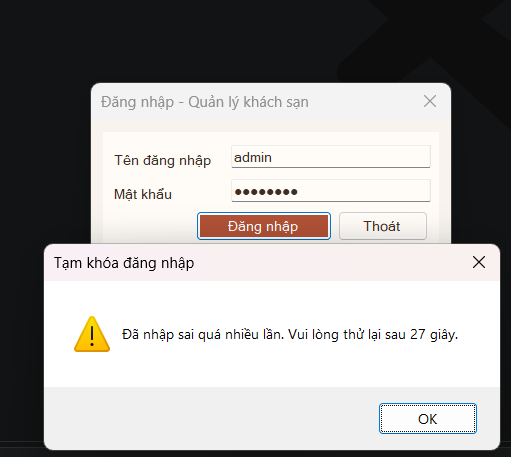
\includegraphics[width=0.6\textwidth]{SpamLock.png}}}{\fbox{\parbox{0.6\textwidth}{\centering\vspace{3cm}\textit{(Chèn ảnh chụp màn hình: SpamLock.png)}\vspace{3cm}}}}}
\caption{Màn hình đăng nhập}
\label{fig:gui-login}
\end{figure}

Màn hình tối giản, chỉ gồm hai ô nhập và một nút xác nhận; khi tài khoản bị khóa tạm thời do đăng nhập sai nhiều lần, thông báo hiển thị rõ thời gian còn lại thay vì chỉ báo "sai mật khẩu" chung chung, giúp người dùng hiểu đúng nguyên nhân.

\section{Màn hình chính (FrmMain)}

\begin{figure}[H]
\centering
{\setlength{\fboxsep}{0pt}%
\IfFileExists{FormMainLT.png}{\fbox{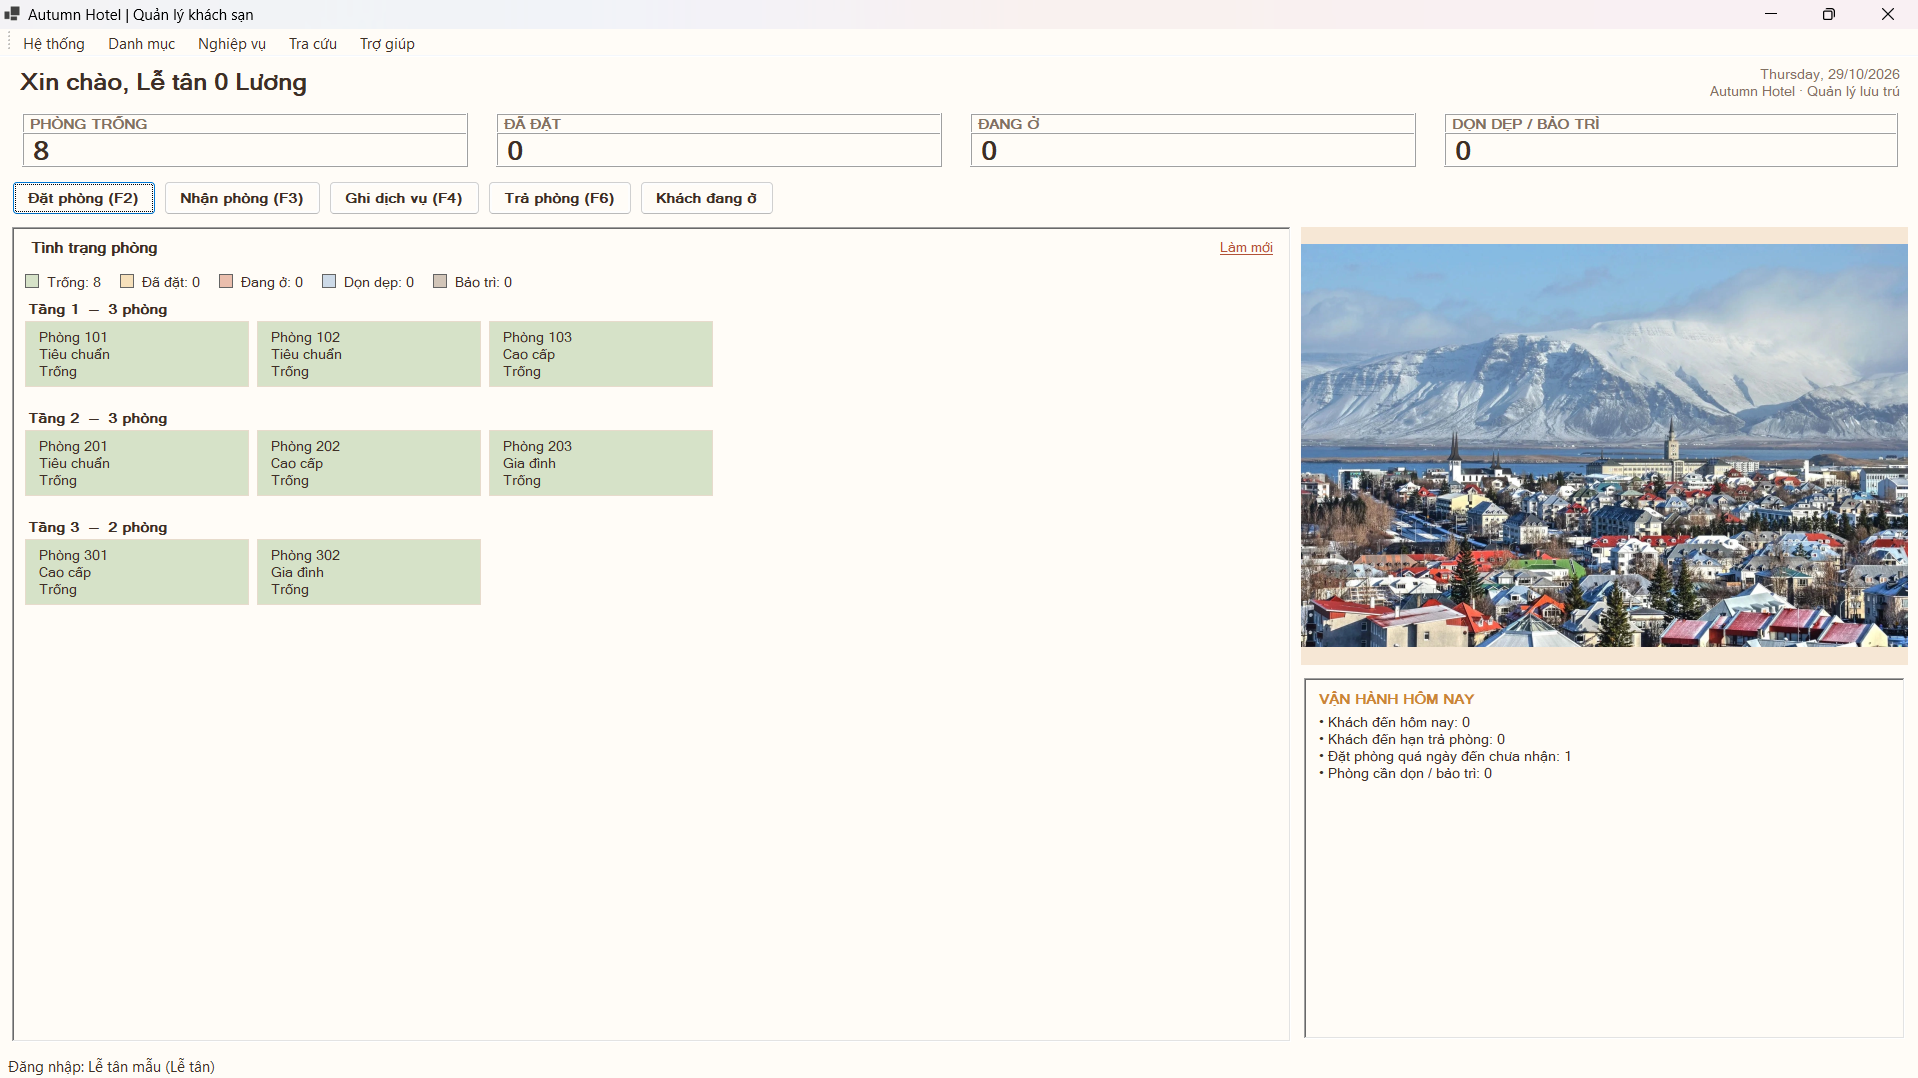
\includegraphics[width=1\textwidth]{FormMainLT.png}}}{\fbox{\parbox{1\textwidth}{\centering\vspace{3cm}\textit{(Chèn ảnh chụp màn hình: FormMainLT.png)}\vspace{3cm}}}}}
\caption{Màn hình đăng nhập lễ tân}
\label{fig:gui-main}
\end{figure}

\begin{figure}[H]
\centering
{\setlength{\fboxsep}{0pt}%
\IfFileExists{FormMainQL.png}{\fbox{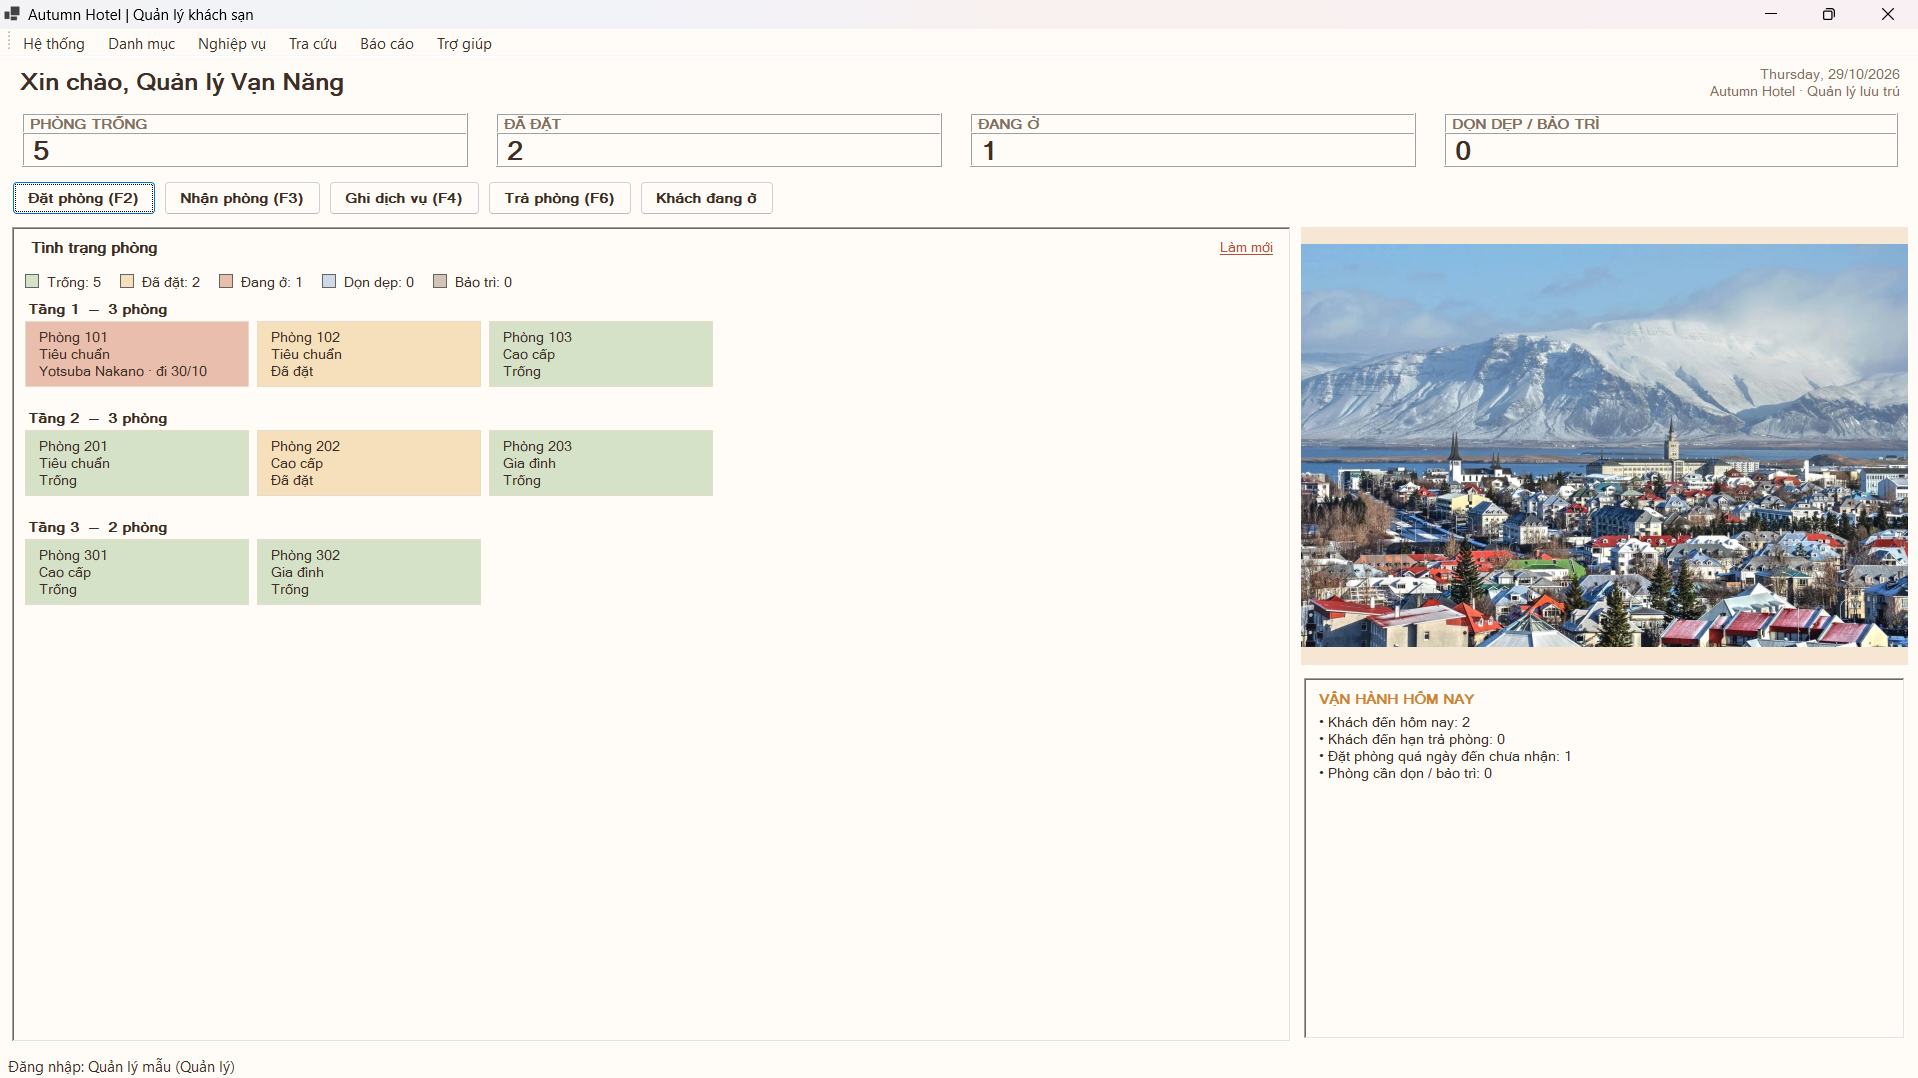
\includegraphics[width=1\textwidth]{FormMainQL.png}}}{\fbox{\parbox{1\textwidth}{\centering\vspace{3cm}\textit{(Chèn ảnh chụp màn hình: FormMainQL.png)}\vspace{3cm}}}}}
\caption{Màn hình đăng nhập quản lý}
\label{fig:gui-main-2}
\end{figure}

Màn hình chính đóng vai trò trung tâm điều hướng, hiển thị ngay các chỉ số vận hành quan trọng nhất (số phòng trống, số khách đang lưu trú, doanh thu trong ngày), giúp lễ tân nắm bắt tình hình tức thời khi vào ca.

\section{Sơ đồ phòng theo tầng}

\begin{figure}[H]
\centering
{\setlength{\fboxsep}{0pt}%
\IfFileExists{SoDo.png}{\fbox{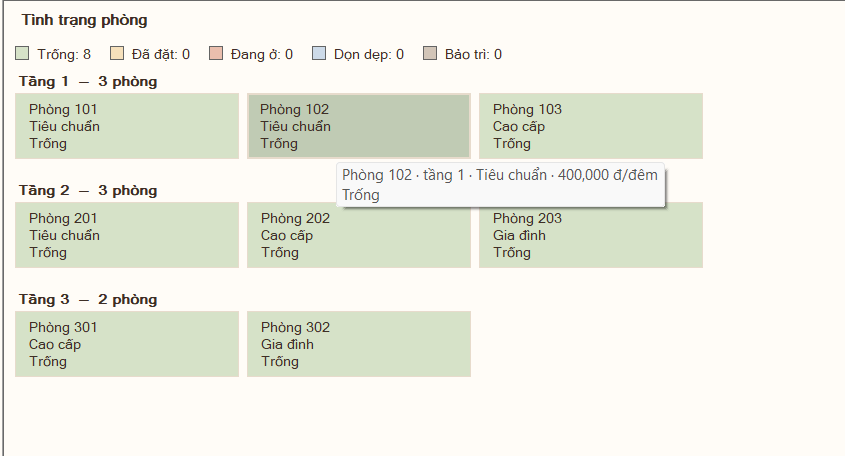
\includegraphics[width=1\textwidth]{SoDo.png}}}{\fbox{\parbox{1\textwidth}{\centering\vspace{3cm}\textit{(Chèn ảnh chụp màn hình: SoDo.png)}\vspace{3cm}}}}}
\caption{Màn hình sơ đồ phòng trống}
\label{fig:gui-sodophong}
\end{figure}

\begin{figure}[H]
\centering
{\setlength{\fboxsep}{0pt}%
\IfFileExists{SoDoDaDat.png}{\fbox{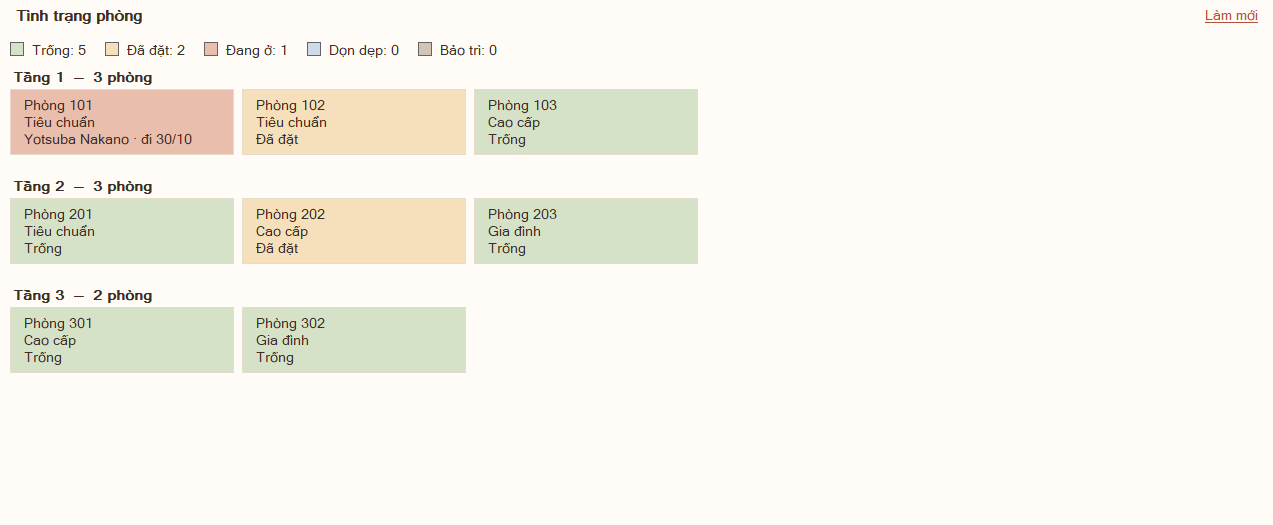
\includegraphics[width=1\textwidth]{SoDoDaDat.png}}}{\fbox{\parbox{1\textwidth}{\centering\vspace{3cm}\textit{(Chèn ảnh chụp màn hình: SoDoDaDat.png)}\vspace{3cm}}}}}
\caption{Màn hình sơ đồ phòng đã đặt}
\label{fig:gui-login-2}
\end{figure}

Sơ đồ phòng là màn hình được truy cập nhiều nhất trong ca trực, nên được thiết kế để một cái nhìn là đủ nắm toàn bộ trạng thái khách sạn; màu sắc trạng thái tuân theo quy ước nhất quán với bảng màu đã định nghĩa trong \texttt{docs/02\_QuyTrinh\_NghiepVu.md} và được dùng lại ở mọi nơi khác hiển thị trạng thái phòng (danh sách phòng, màn hình đặt phòng).

\section{Màn hình Đặt phòng (F2)}

\begin{figure}[H]
\centering
{\setlength{\fboxsep}{0pt}%
\IfFileExists{OrderRoom.png}{\fbox{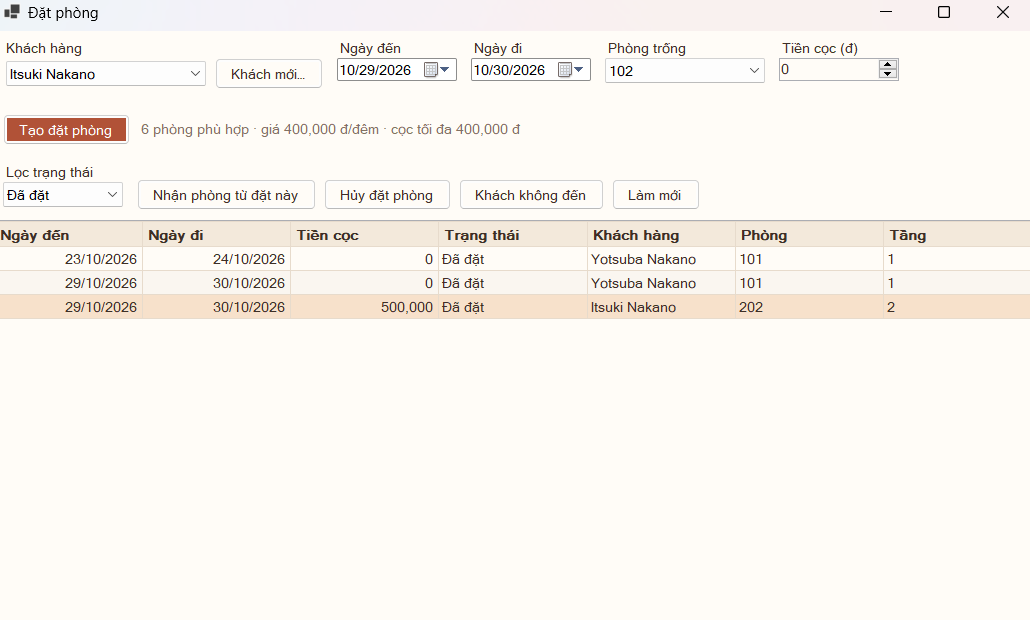
\includegraphics[width=1\textwidth]{OrderRoom.png}}}{\fbox{\parbox{1\textwidth}{\centering\vspace{3cm}\textit{(Chèn ảnh chụp màn hình: OrderRoom.png)}\vspace{3cm}}}}}
\caption{Màn hình đặt phòng}
\label{fig:gui-datphong}
\end{figure}

Danh sách phòng chỉ hiển thị các phòng thỏa điều kiện khả dụng cho đúng khoảng ngày đang chọn (không bảo trì, không trùng lịch), giúp người dùng không thể chọn nhầm một phòng rồi mới nhận được thông báo lỗi ở bước lưu.

\begin{figure}[H]
\centering
{\setlength{\fboxsep}{0pt}%
\IfFileExists{ODSuccess.png}{\fbox{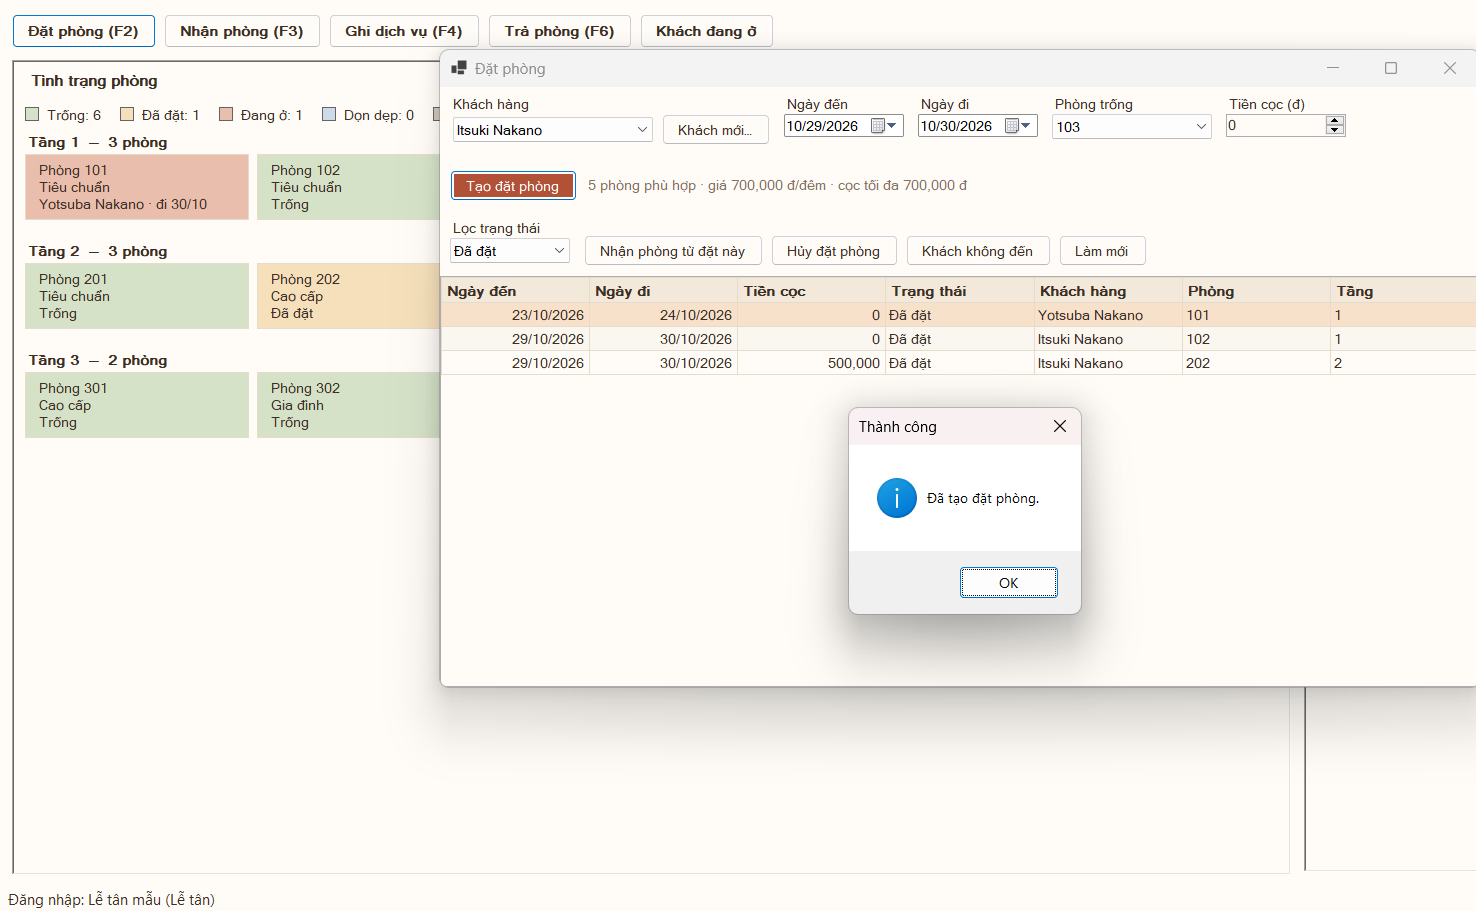
\includegraphics[width=1\textwidth]{ODSuccess.png}}}{\fbox{\parbox{1\textwidth}{\centering\vspace{3cm}\textit{(Chèn ảnh chụp màn hình: ODSuccess.png)}\vspace{3cm}}}}}
\caption{Màn hình đặt phòng thành công}
\label{fig:gui-datphong-2}
\end{figure}

Khi Lễ tân nhập mức giảm vượt 10\% tiền hàng (phòng, dịch vụ, phụ thu) và bấm trả phòng, hệ thống mở hộp thoại \textit{Quản lý duyệt giảm giá}. Quản lý nhập tên đăng nhập và mật khẩu của mình; chỉ tài khoản đang hoạt động có vai trò Quản lý mới được chấp nhận, nếu không thao tác trả phòng bị hủy. Khi người dùng đang đăng nhập đã là Quản lý thì không hiện hộp thoại và người đó được ghi là người duyệt. Hóa đơn lưu mã người duyệt, đồng thời bản in có dòng \textit{Quản lý duyệt giảm giá}.

\begin{figure}[H]
\centering
{\setlength{\fboxsep}{0pt}%
\IfFileExists{DuyetGiamGia.png}{\fbox{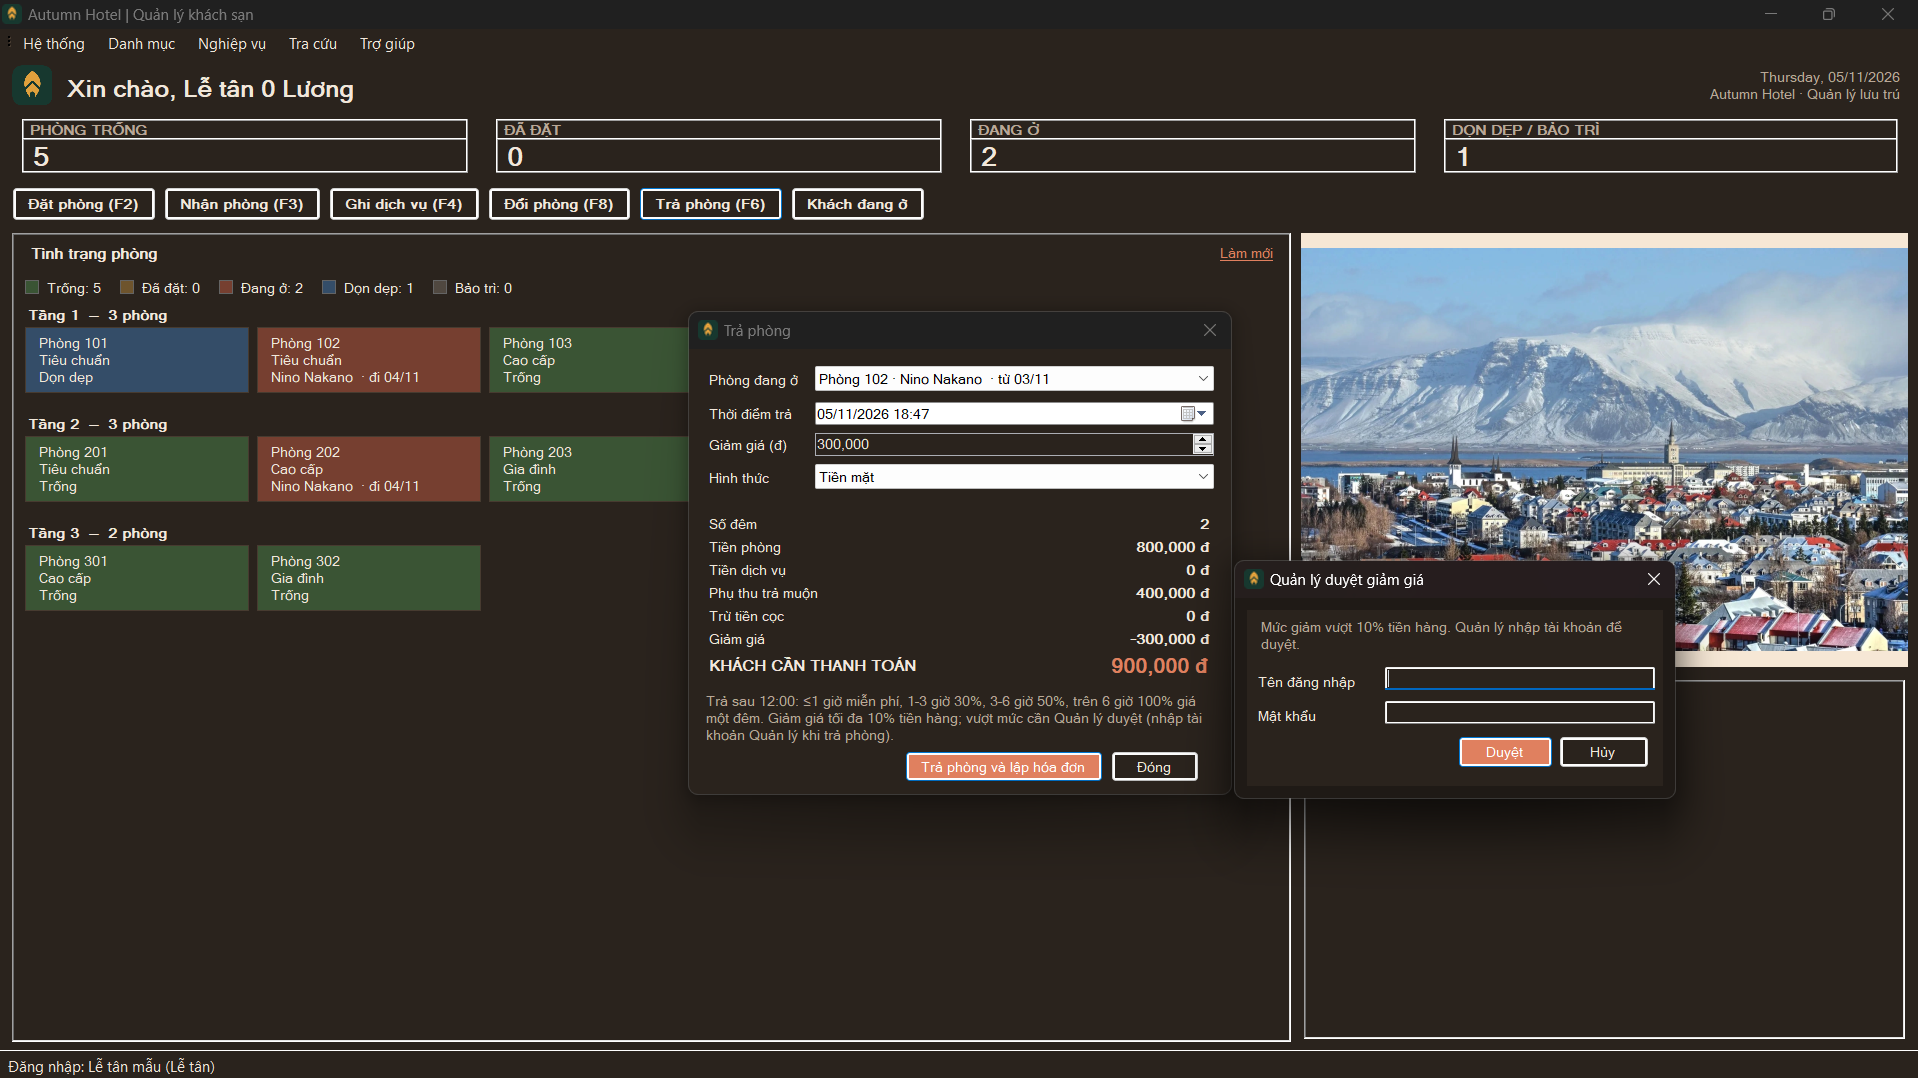
\includegraphics[width=1\textwidth]{DuyetGiamGia.png}}}{\fbox{\parbox{1\textwidth}{\centering\vspace{3cm}\textit{(Chèn ảnh chụp màn hình: DuyetGiamGia.png)}\vspace{3cm}}}}}
\caption{Hộp thoại Quản lý duyệt giảm giá}
\label{fig:gui-duyetgiamgia}
\end{figure}

\begin{figure}[H]
\centering
{\setlength{\fboxsep}{0pt}%
\IfFileExists{QLDuyetGiamGia.png}{\fbox{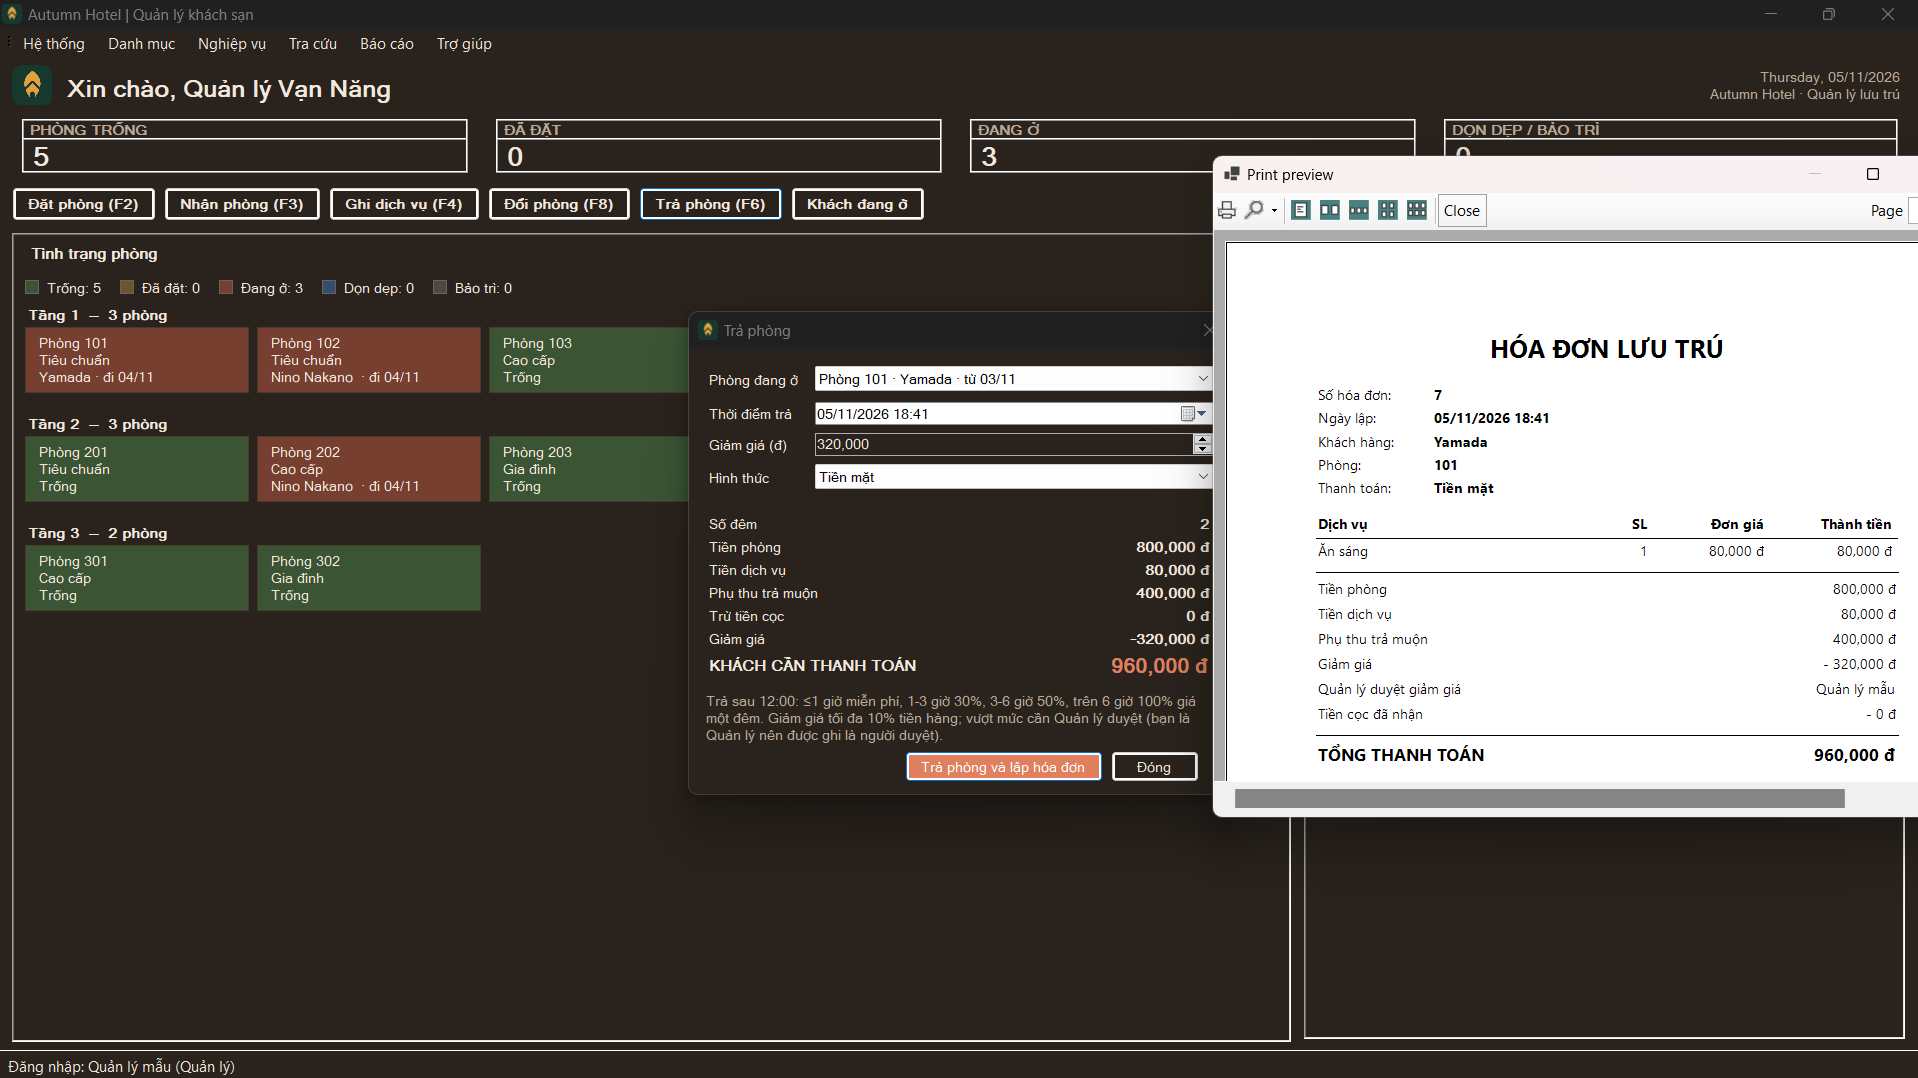
\includegraphics[width=1\textwidth]{QLDuyetGiamGia.png}}}{\fbox{\parbox{1\textwidth}{\centering\vspace{3cm}\textit{(Chèn ảnh chụp màn hình: QLDuyetGiamGia.png)}\vspace{3cm}}}}}
\caption{Quản lý trực tiếp giảm giá}
\label{fig:gui-duyetgiamgia-2}
\end{figure}

\section{Màn hình Nhận phòng (F3) và Ghi dịch vụ (F4)}

\begin{figure}[H]
\centering
{\setlength{\fboxsep}{0pt}%
\IfFileExists{F3.png}{\fbox{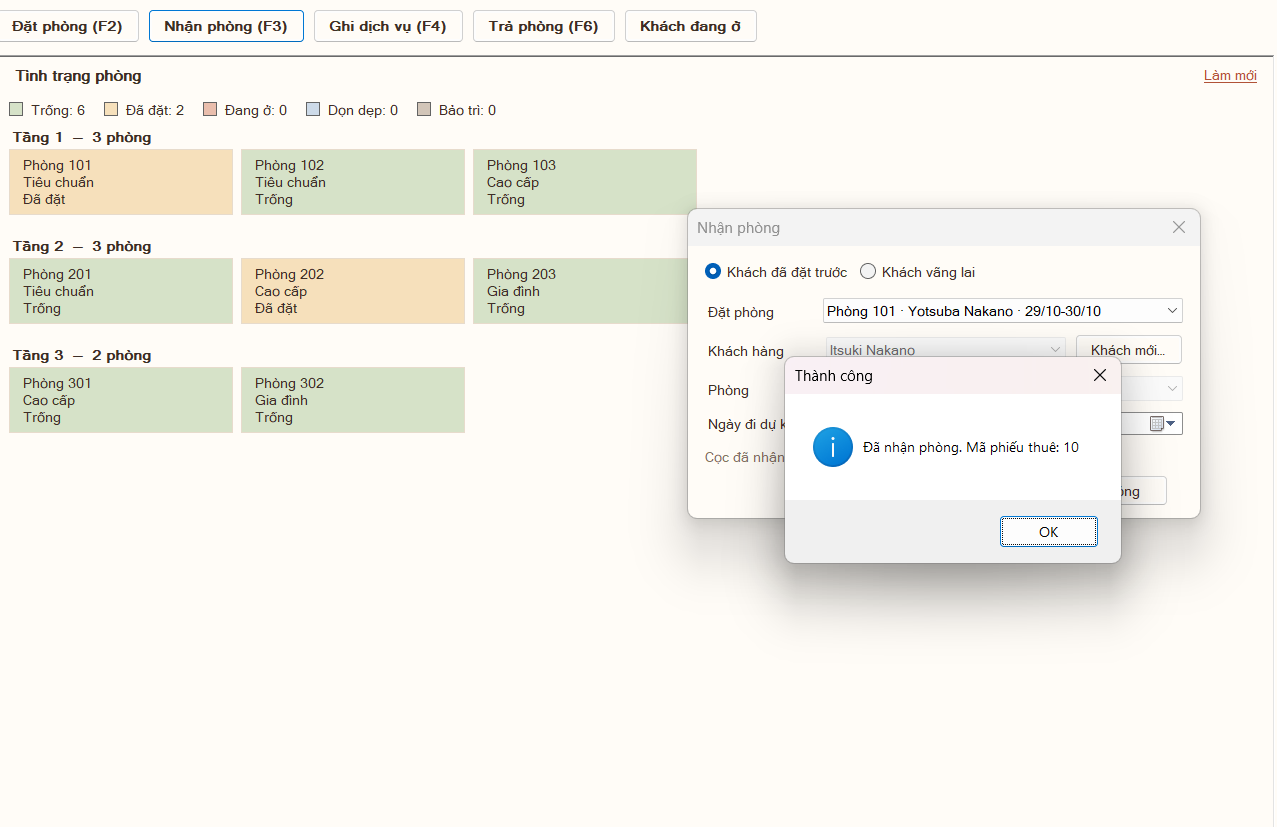
\includegraphics[width=1\textwidth]{F3.png}}}{\fbox{\parbox{1\textwidth}{\centering\vspace{3cm}\textit{(Chèn ảnh chụp màn hình: F3.png)}\vspace{3cm}}}}}
\caption{Màn hình nhận phòng}
\label{fig:gui-nhanphong-dichvu}
\end{figure}

\begin{figure}[H]
\centering
{\setlength{\fboxsep}{0pt}%
\IfFileExists{F4.png}{\fbox{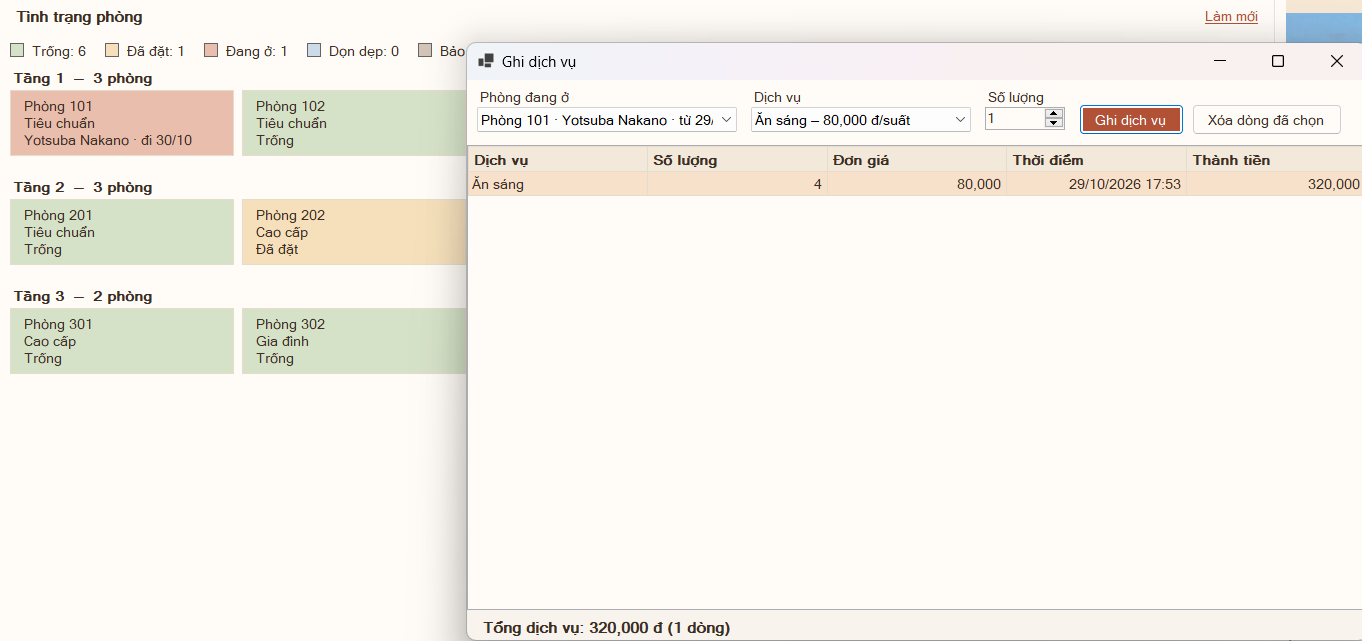
\includegraphics[width=1\textwidth]{F4.png}}}{\fbox{\parbox{1\textwidth}{\centering\vspace{3cm}\textit{(Chèn ảnh chụp màn hình: F4.png)}\vspace{3cm}}}}}
\caption{Màn hình ghi dịch vụ}
\label{fig:gui-nhanphong-dichvu-2}
\end{figure}

\section{Màn hình Trả phòng (F6) và xem trước hóa đơn}

\begin{figure}[H]
\centering
{\setlength{\fboxsep}{0pt}%
\IfFileExists{F6.png}{\fbox{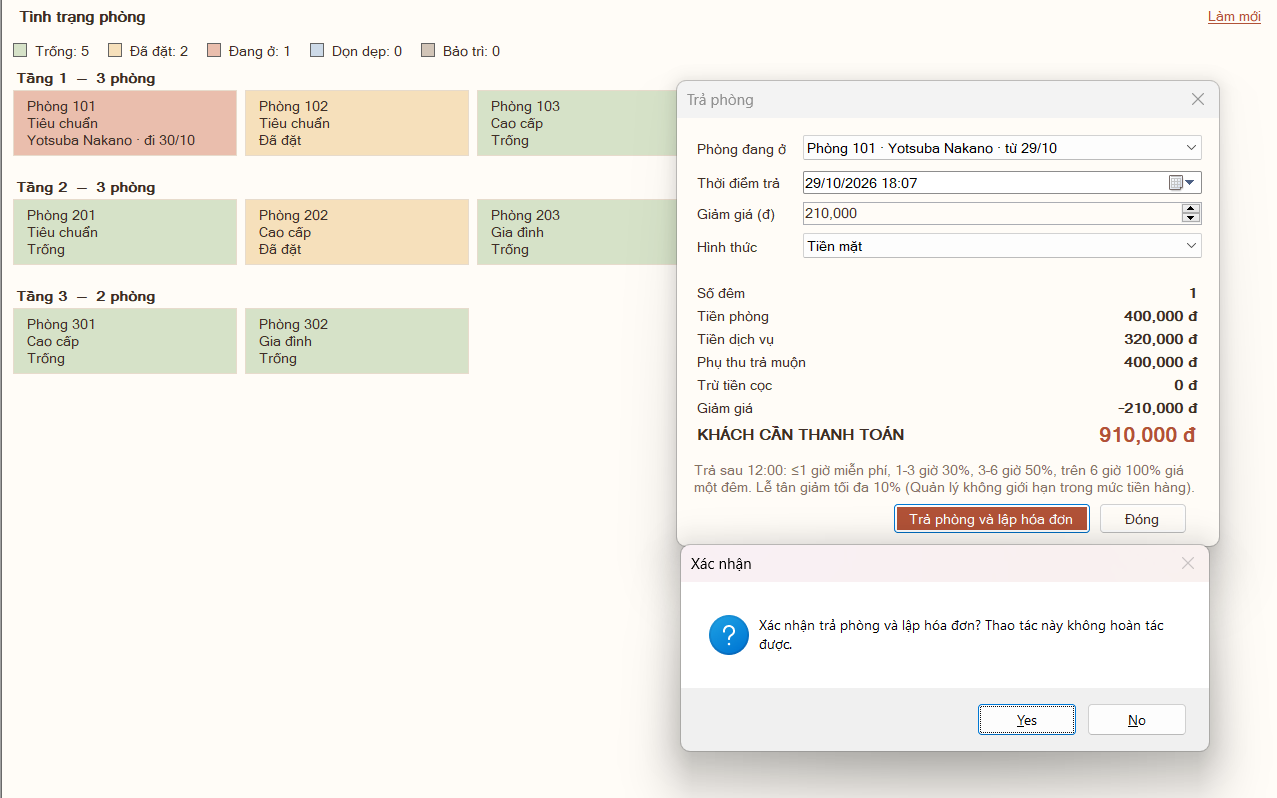
\includegraphics[width=1\textwidth]{F6.png}}}{\fbox{\parbox{1\textwidth}{\centering\vspace{3cm}\textit{(Chèn ảnh chụp màn hình: F6.png)}\vspace{3cm}}}}}
\caption{Màn hình trả phòng}
\label{fig:gui-traphong}
\end{figure}

Bảng chi tiết tính tiền được tính lại tức thời mỗi khi người dùng thay đổi mức giảm giá, giúp lễ tân thấy ngay ảnh hưởng trước khi xác nhận, giảm thao tác thử sai.

\begin{figure}[H]
\centering
{\setlength{\fboxsep}{0pt}%
\IfFileExists{Bill.png}{\fbox{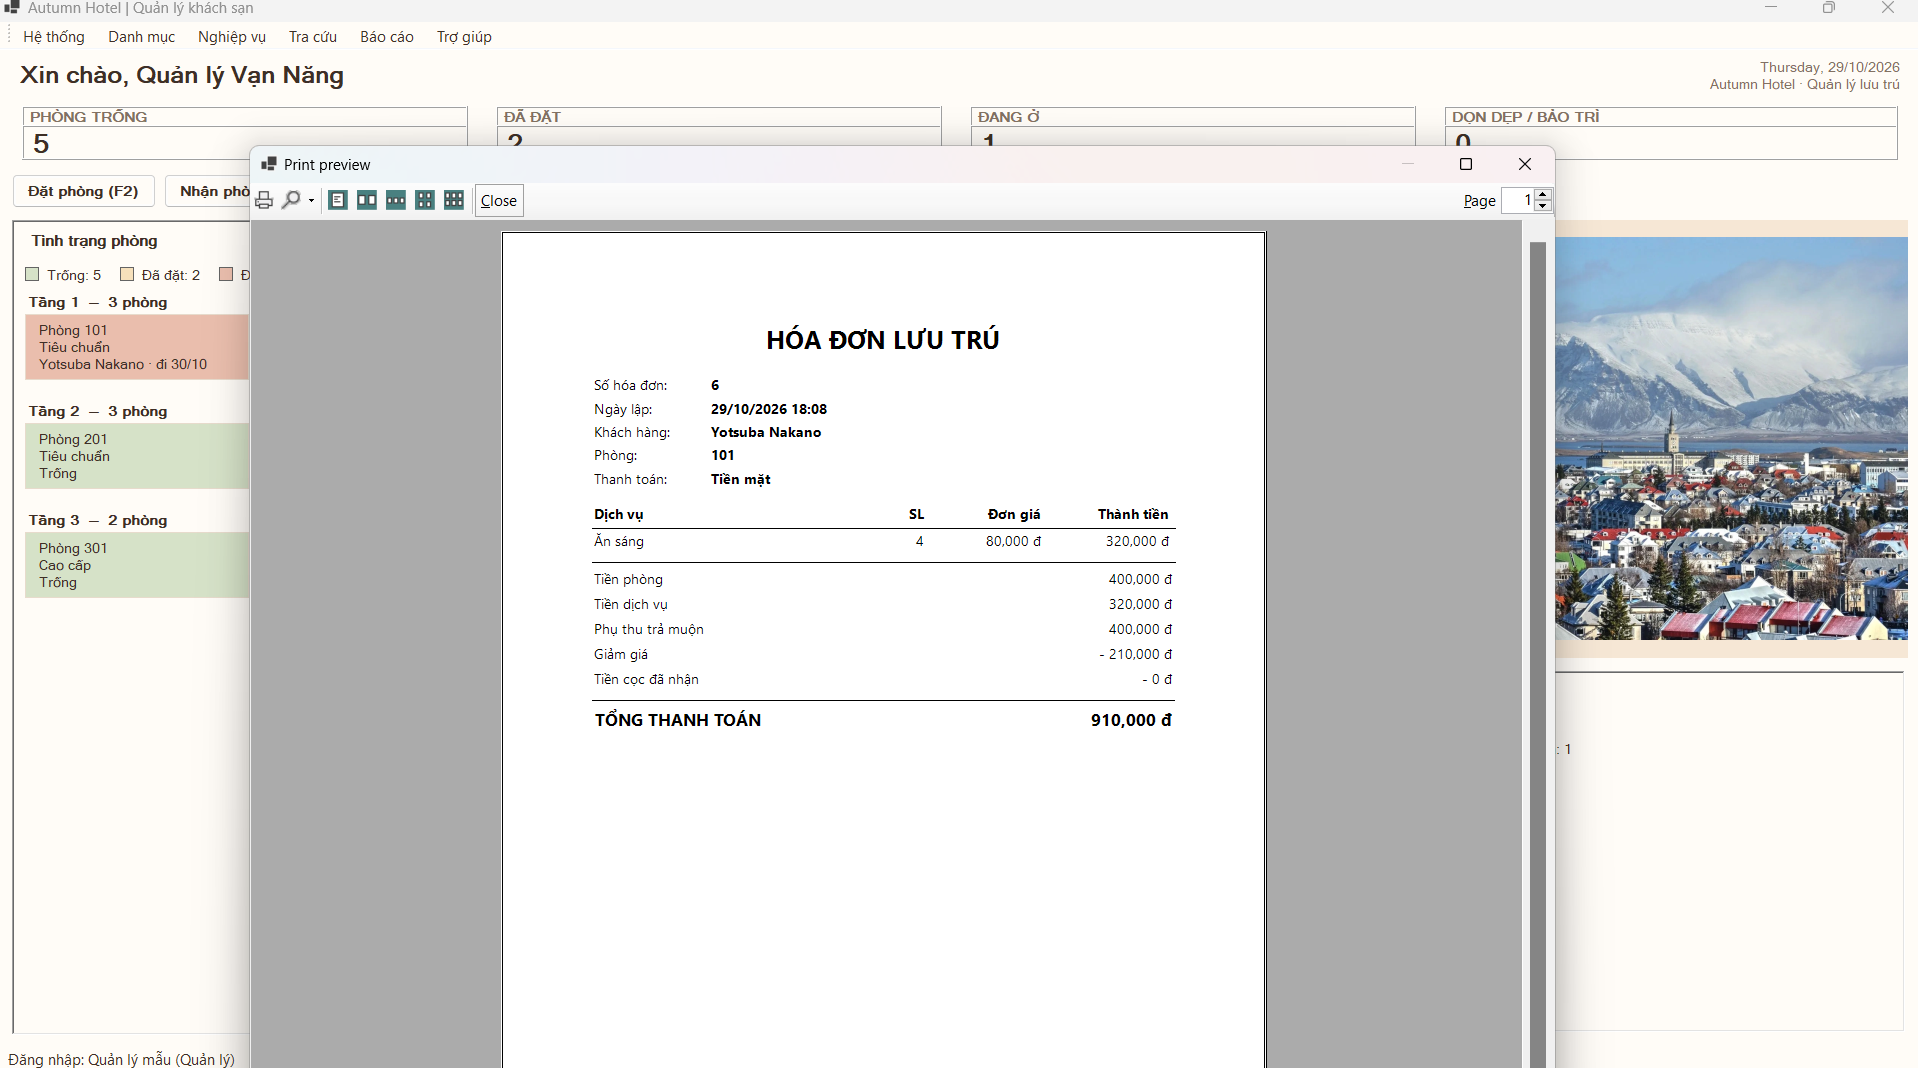
\includegraphics[width=1\textwidth]{Bill.png}}}{\fbox{\parbox{1\textwidth}{\centering\vspace{3cm}\textit{(Chèn ảnh chụp màn hình: Bill.png)}\vspace{3cm}}}}}
\caption{Màn hình in hóa đơn}
\label{fig:gui-traphong-2}
\end{figure}

\section{Màn hình Đổi phòng (F8)}

Màn hình cho phép đổi phòng khi khách đang lưu trú (UC23). Lễ tân chọn phòng đang có khách, chọn phòng mới trong danh sách các phòng còn trống trọn thời gian còn lại của kỳ lưu trú (kèm tầng, loại phòng và giá), có thể nhập lý do (tối đa 200 ký tự) rồi bấm \textit{Đổi phòng}. Dòng nhắc bên dưới cho biết phòng mới cùng mức giá hay khác giá; đơn giá của phiếu thuê được giữ nguyên (QT49) và chênh lệch xử lý khi trả phòng. Bảng phía dưới liệt kê lịch sử đổi phòng của phiếu thuê đang chọn (thời điểm, phòng cũ, phòng mới, giá, lý do).

\begin{figure}[H]
\centering
{\setlength{\fboxsep}{0pt}%
\IfFileExists{F8.png}{\fbox{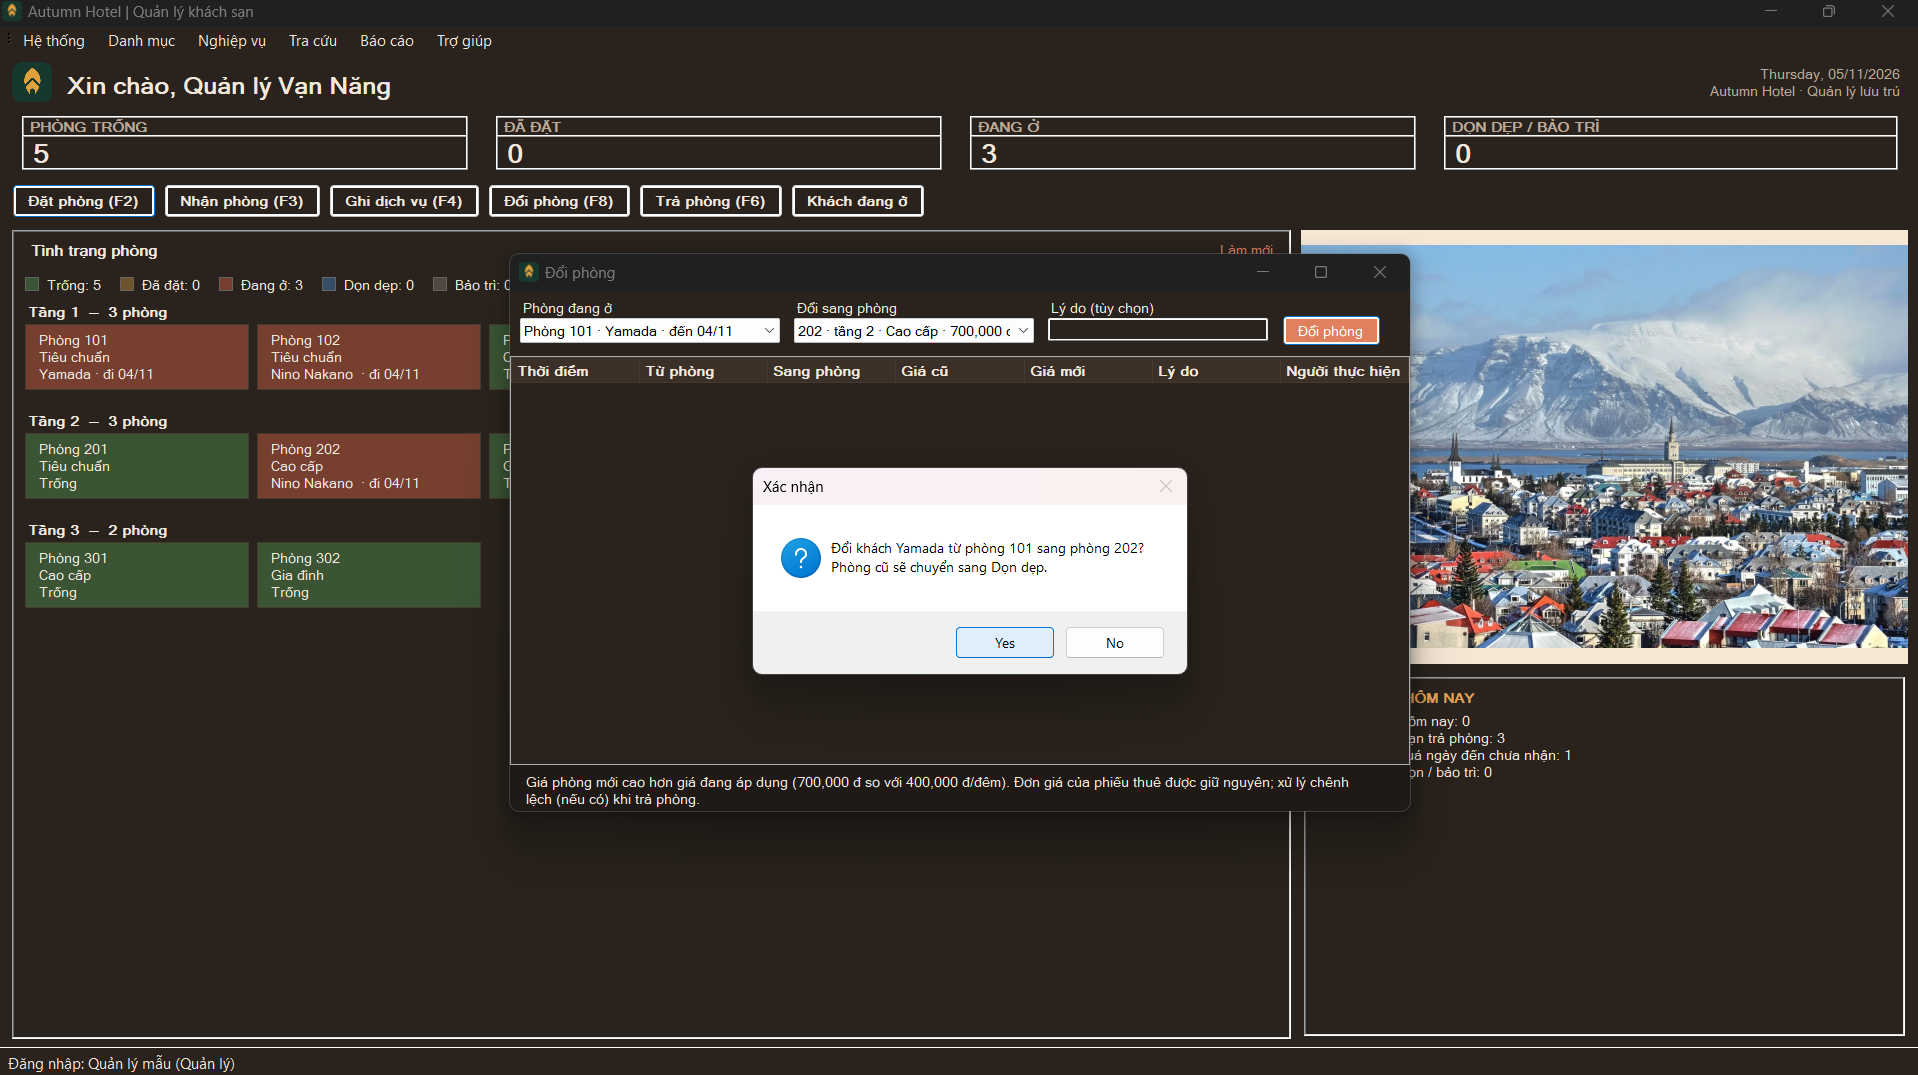
\includegraphics[width=1\textwidth]{F8.png}}}{\fbox{\parbox{1\textwidth}{\centering\vspace{3cm}\textit{(Chèn ảnh chụp màn hình: F8.png)}\vspace{3cm}}}}}
\caption{Màn hình đổi phòng}
\label{fig:gui-doiphong}
\end{figure}

\section{Màn hình Báo cáo doanh thu và công suất phòng}

\begin{figure}[H]
\centering
{\setlength{\fboxsep}{0pt}%
\IfFileExists{Profit.png}{\fbox{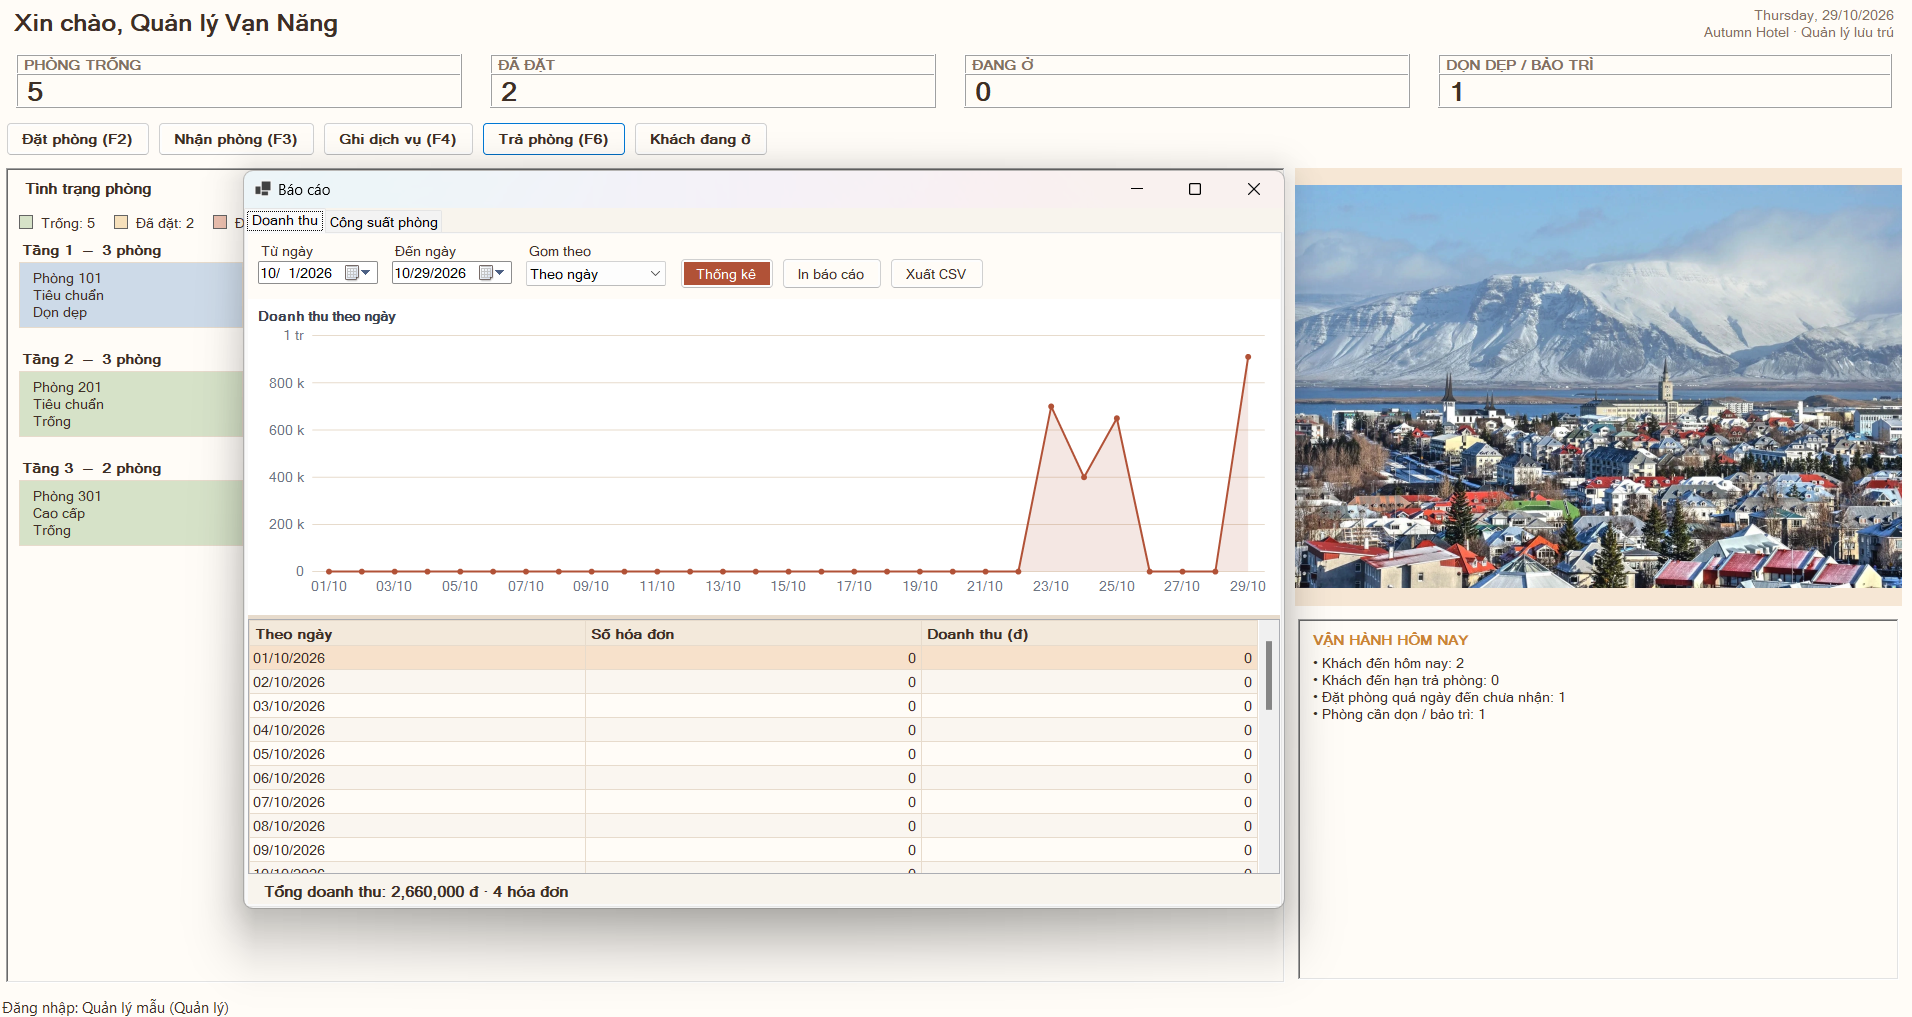
\includegraphics[width=1\textwidth]{Profit.png}}}{\fbox{\parbox{1\textwidth}{\centering\vspace{3cm}\textit{(Chèn ảnh chụp màn hình: Profit.png)}\vspace{3cm}}}}}
\caption{Màn hình báo cáo doanh thu}
\label{fig:gui-baocao}
\end{figure}

Biểu đồ được vẽ trực tiếp bằng GDI+ (lớp \texttt{ChartPanel} tự xây dựng) thay vì phụ thuộc thư viện biểu đồ ngoài, giữ ứng dụng nhẹ và không phát sinh phụ thuộc bên ngoài. Dữ liệu gom nhóm bao gồm cả các mốc thời gian không phát sinh doanh thu, giúp biểu đồ phản ánh đúng xu hướng liên tục.

\begin{figure}[H]
\centering
{\setlength{\fboxsep}{0pt}%
\IfFileExists{OR.png}{\fbox{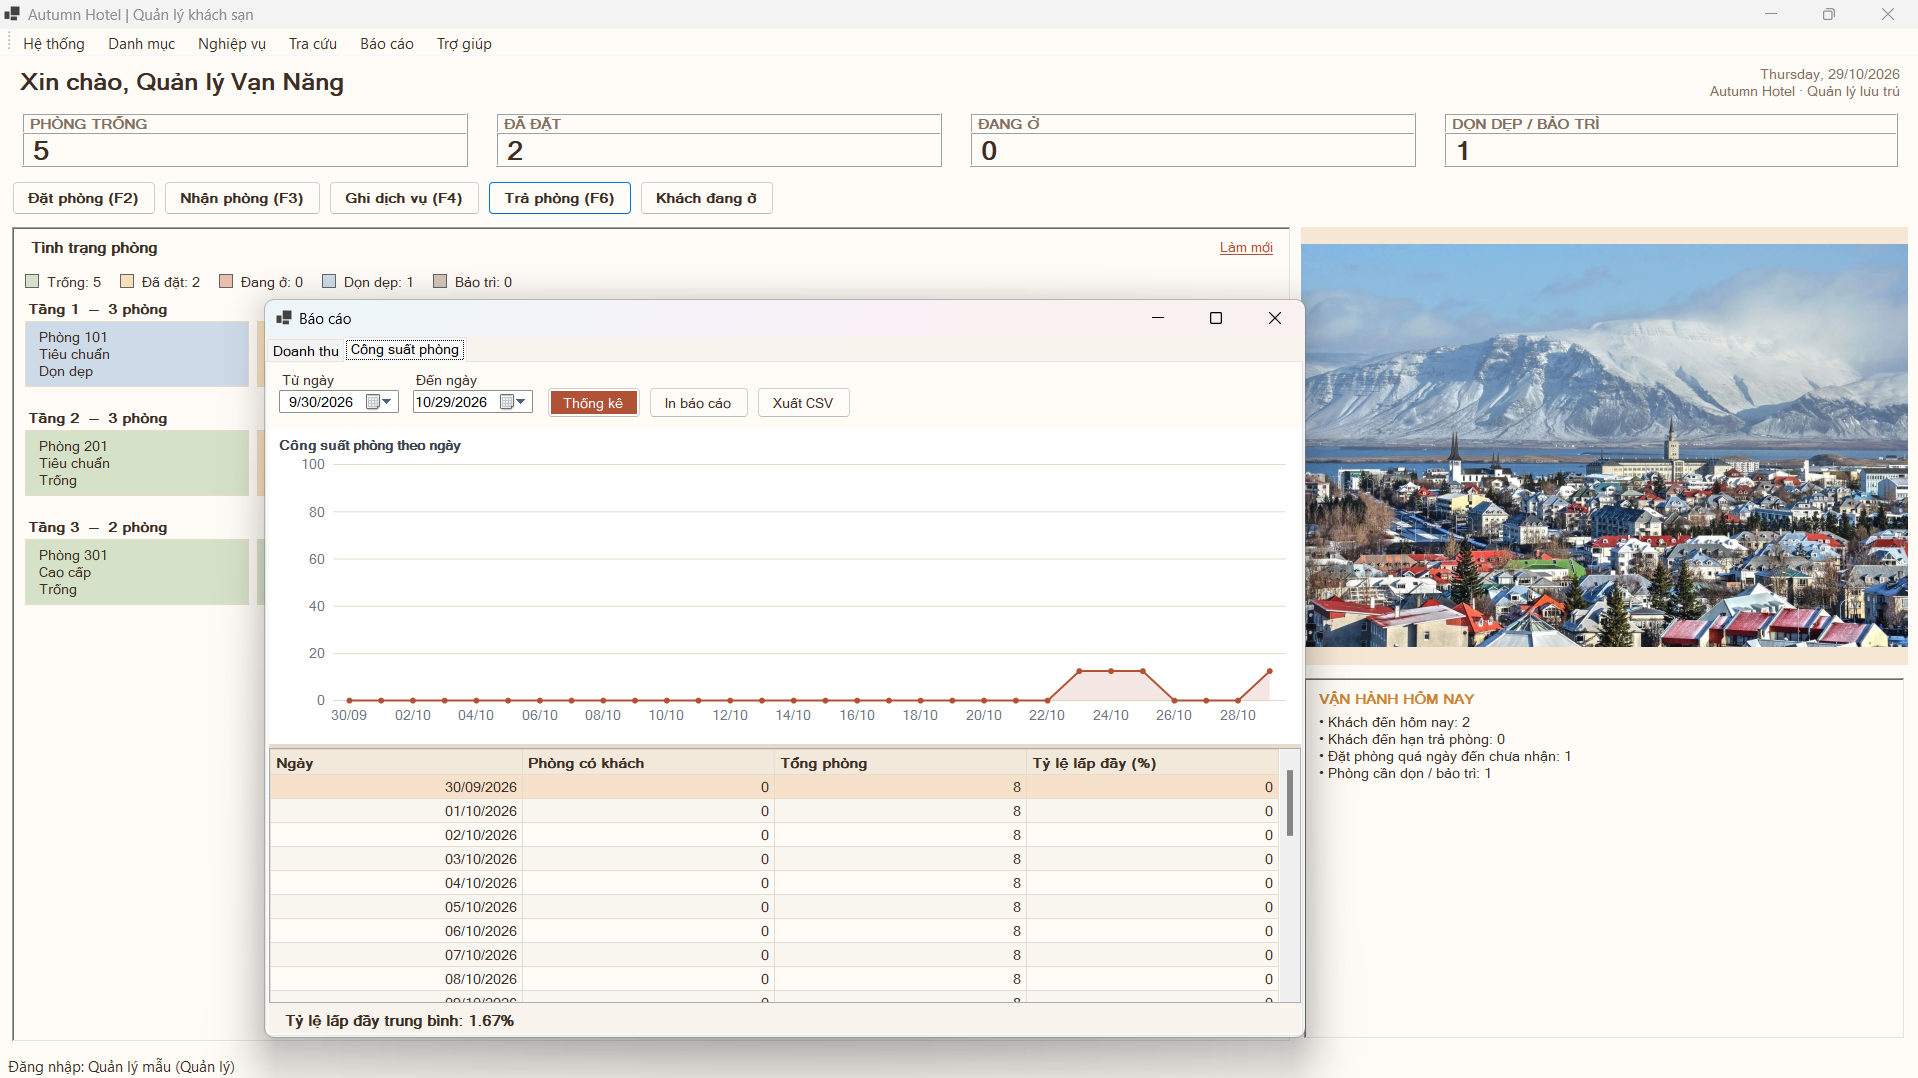
\includegraphics[width=1\textwidth]{OR.png}}}{\fbox{\parbox{1\textwidth}{\centering\vspace{3cm}\textit{(Chèn ảnh chụp màn hình: OR.png)}\vspace{3cm}}}}}
\caption{Màn hình công suất phòng}
\label{fig:gui-baocao-2}
\end{figure}

\section{Các màn hình danh mục}

\begin{figure}[H]
\centering
{\setlength{\fboxsep}{0pt}%
\IfFileExists{Phong.png}{\fbox{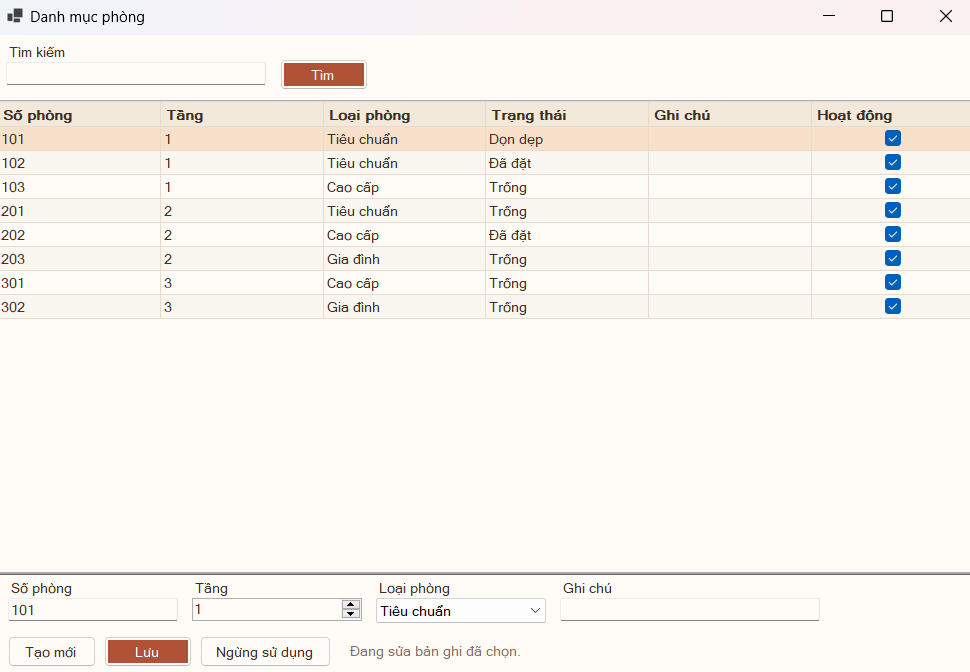
\includegraphics[width=0.9\textwidth]{Phong.png}}}{\fbox{\parbox{0.9\textwidth}{\centering\vspace{3cm}\textit{(Chèn ảnh chụp màn hình: Phong.png)}\vspace{3cm}}}}}
\caption{Danh mục phòng}
\label{fig:gui-danhmuc}
\end{figure}

\begin{figure}[H]
\centering
{\setlength{\fboxsep}{0pt}%
\IfFileExists{KH.png}{\fbox{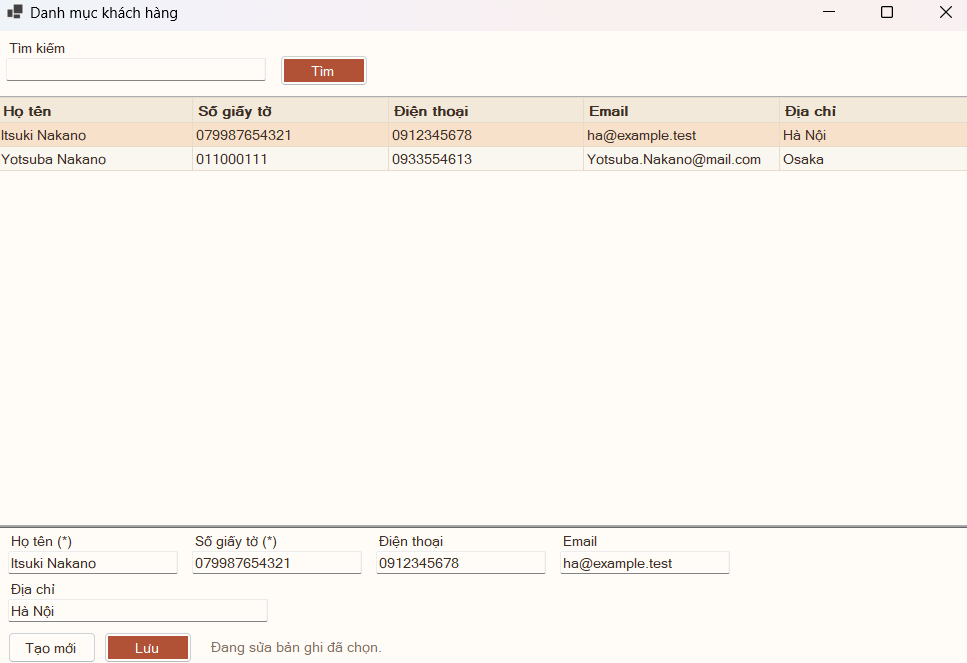
\includegraphics[width=0.9\textwidth]{KH.png}}}{\fbox{\parbox{0.9\textwidth}{\centering\vspace{3cm}\textit{(Chèn ảnh chụp màn hình: KH.png)}\vspace{3cm}}}}}
\caption{Danh mục khách hàng}
\label{fig:gui-danhmuc-2}
\end{figure}

\begin{figure}[H]
\centering
{\setlength{\fboxsep}{0pt}%
\IfFileExists{DichVu.png}{\fbox{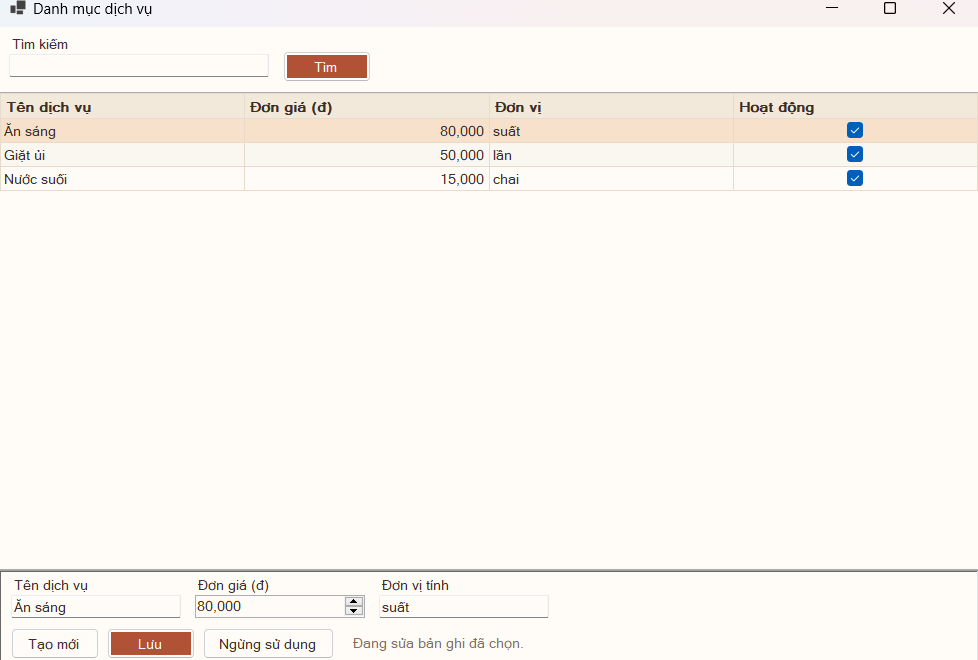
\includegraphics[width=0.9\textwidth]{DichVu.png}}}{\fbox{\parbox{0.9\textwidth}{\centering\vspace{3cm}\textit{(Chèn ảnh chụp màn hình: DichVu.png)}\vspace{3cm}}}}}
\caption{Danh mục dịch vụ}
\label{fig:gui-danhmuc-3}
\end{figure}

\section{Màn hình Quản lý tài khoản (chỉ Quản lý)}

\begin{figure}[H]
\centering
{\setlength{\fboxsep}{0pt}%
\IfFileExists{QLTK.png}{\fbox{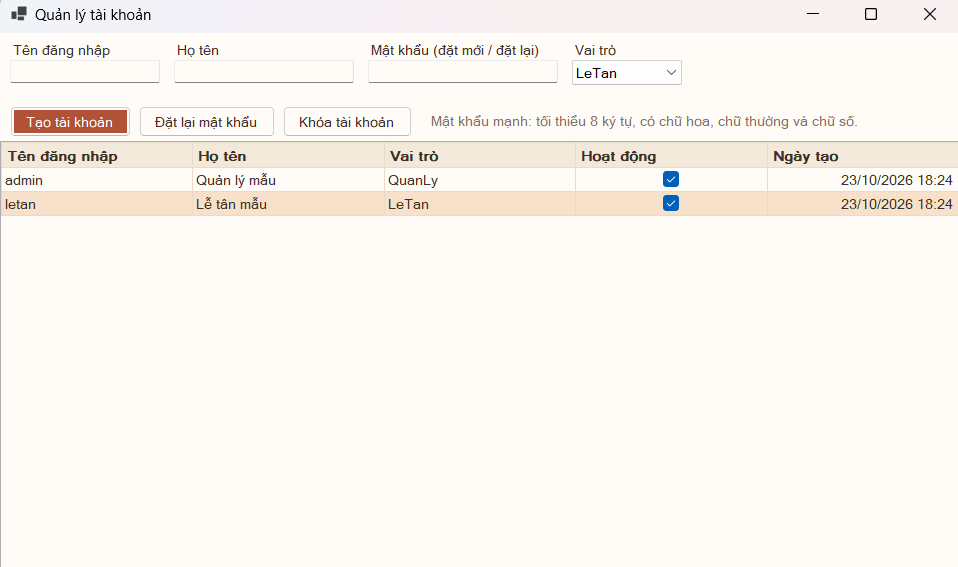
\includegraphics[width=0.9\textwidth]{QLTK.png}}}{\fbox{\parbox{0.9\textwidth}{\centering\vspace{3cm}\textit{(Chèn ảnh chụp màn hình: QLTK.png)}\vspace{3cm}}}}}
\caption{Màn hình quản lý tài khoản}
\label{fig:gui-danhmuc-4}
\end{figure}

\section{Màn hình Mã QR phòng và giá}

Màn hình \texttt{FrmQrPhong} (menu \textit{Tra cứu $\rightarrow$ Mã QR phòng và giá}) gồm ô chọn nội dung (bảng giá hoặc một phòng), thẻ xem trước chứa mã QR cùng đường dẫn, và hàng nút \textit{Lưu PNG}, \textit{In}, \textit{Xuất tất cả}, \textit{Sao chép liên kết}, \textit{Đóng}. Thẻ xem trước dùng nền trắng cố định kể cả ở chế độ tối để mã luôn dễ quét.

\begin{figure}[H]
\centering
{\setlength{\fboxsep}{0pt}%
\IfFileExists{QrPhong.png}{\fbox{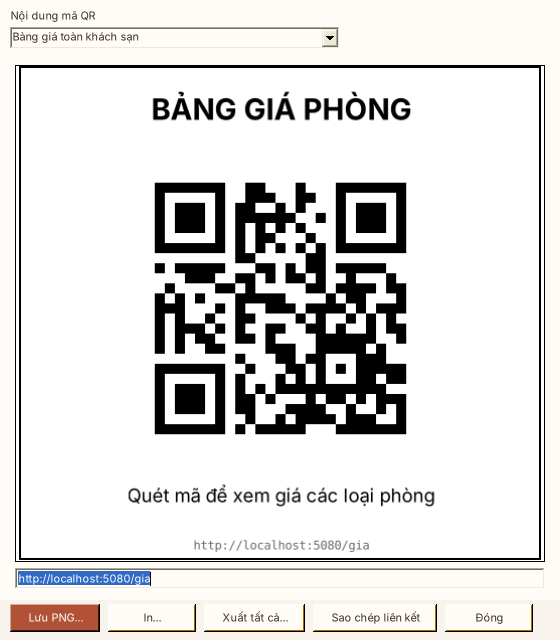
\includegraphics[width=0.6\textwidth]{QrPhong.png}}}{\fbox{\parbox{0.6\textwidth}{\centering\vspace{3cm}\textit{(Chèn ảnh chụp màn hình: QrPhong.png)}\vspace{3cm}}}}}
\caption{Màn hình tạo mã QR}
\label{fig:gui-qr}
\end{figure}

\section{Giao diện tối}

Chế độ tối được bật tại \textit{Hệ thống $\rightarrow$ Giao diện tối} hoặc bằng Ctrl+D; bảng màu nâu ấm đồng bộ với chủ đề thu của ứng dụng. Thẻ phòng giữ ý nghĩa màu theo trạng thái (xanh: trống; vàng: đã đặt; đỏ nâu: đang ở; xanh dương: dọn dẹp; xám: bảo trì) nhưng dùng sắc độ tối hơn để chữ sáng vẫn đủ tương phản.

\begin{figure}[H]
\centering
{\setlength{\fboxsep}{0pt}%
\IfFileExists{FormMainToi.png}{\fbox{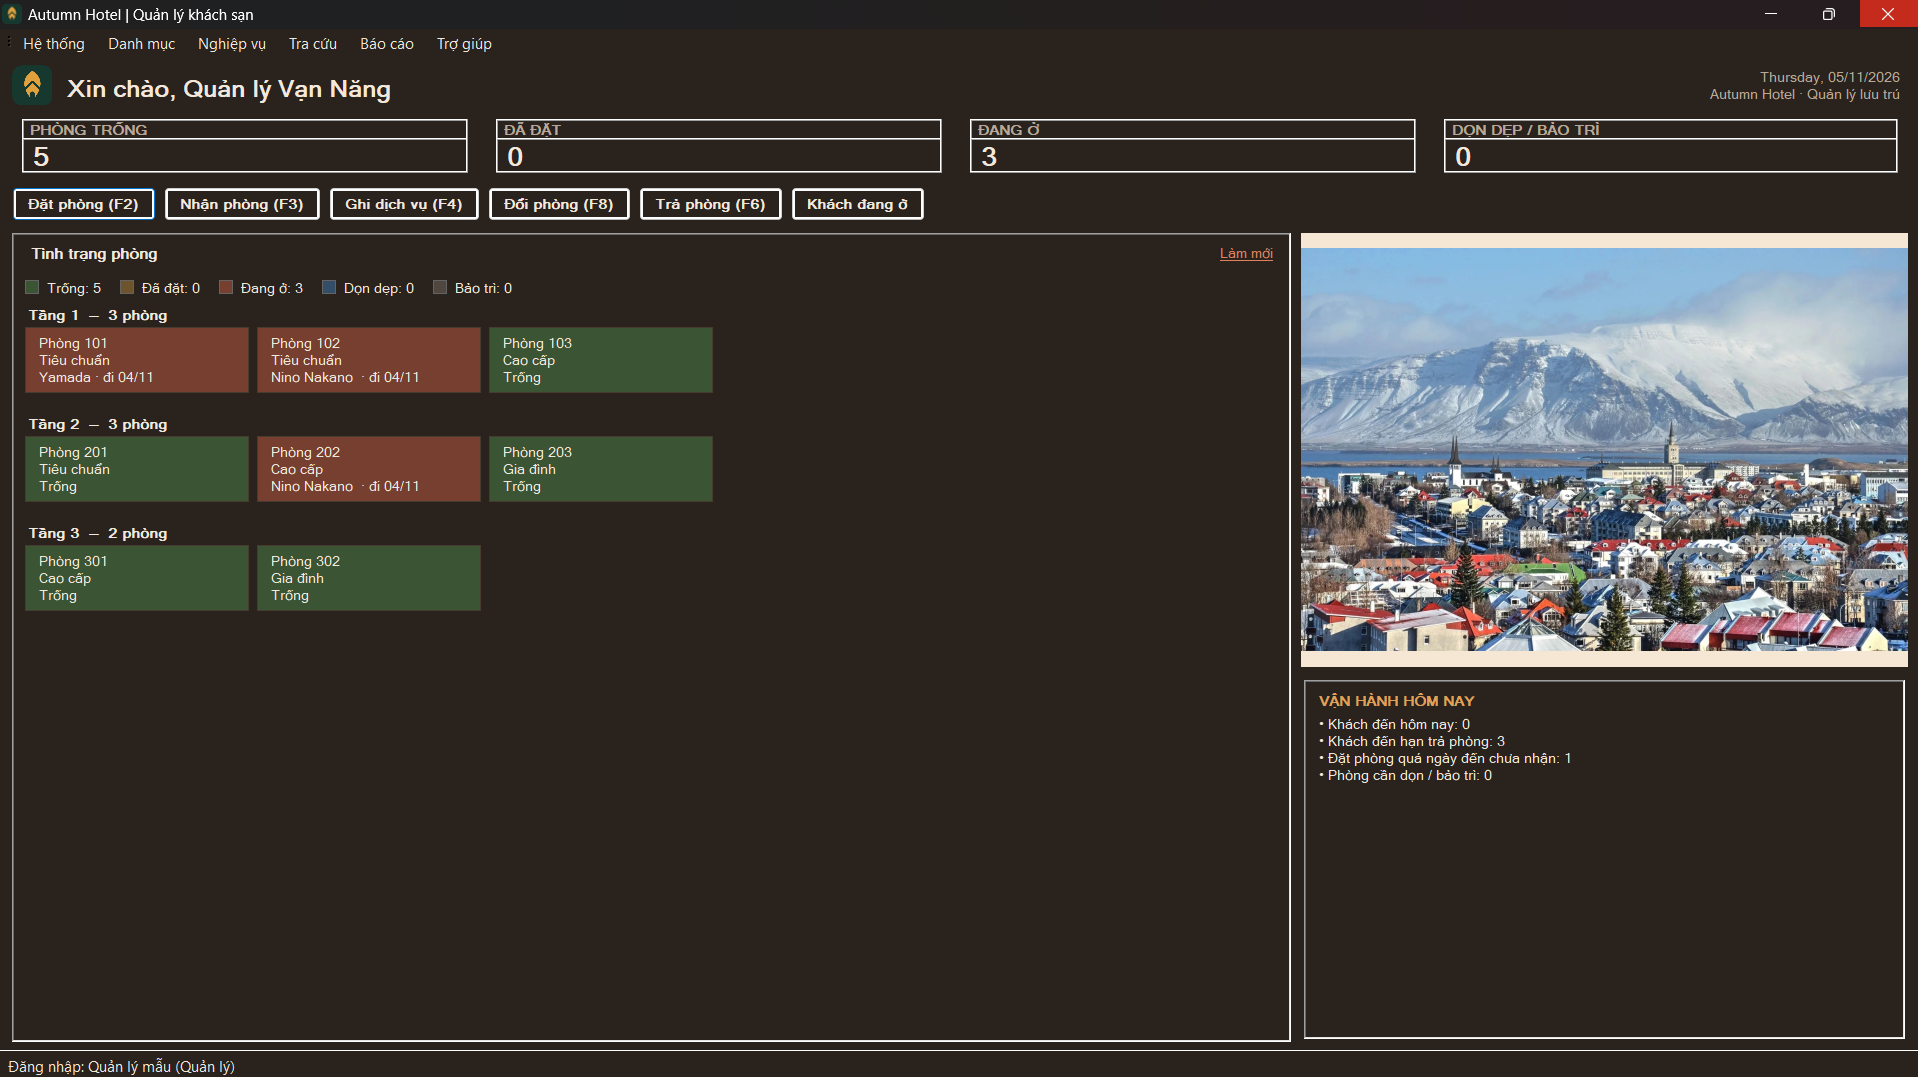
\includegraphics[width=0.8\textwidth]{FormMainToi.png}}}{\fbox{\parbox{0.8\textwidth}{\centering\vspace{3cm}\textit{(Chèn ảnh chụp màn hình: FormMainToi.png)}\vspace{3cm}}}}}
\caption{Màn hình chính ở chế độ tối}
\label{fig:gui-toi}
\end{figure}

\section{Trang web tra cứu trên điện thoại}

Giao diện web dùng bảng màu xanh thông đậm làm màu chủ đạo, hổ phách cho giá, nút và viền focus, nền trang xám phớt xanh; bản tối có bảng màu riêng với nút hổ phách. Các thẻ nổi nhẹ khi rê chuột, dòng bảng đổi màu khi rê, nội dung hiện dần khi vào trang và toàn bộ hiệu ứng được tắt khi thiết bị bật chế độ giảm chuyển động; hiệu ứng chỉ dùng CSS nên không vi phạm chính sách không chạy script. Mỗi loại phòng có hình minh họa vẽ bằng SVG nội tuyến (số giường theo sức chứa, tông màu theo tên loại phòng), nên không cần tải ảnh ngoài và vẫn tuân thủ chính sách chỉ cho phép ảnh cùng nguồn. Trang tìm phòng có hai bộ lọc: loại phòng (danh sách lấy từ bảng giá) và giá tối đa mỗi đêm; kết quả nêu số phòng phù hợp trên tổng số phòng trống và gợi ý nới bộ lọc khi không có phòng nào. Bố cục một cột, thẻ bảng giá tự xếp lưới, ô nhập và nút đủ lớn để chạm, số tiền không bị ngắt dòng. Trang chi tiết phòng (Hình~\ref{fig:web-phong}) hiển thị loại phòng, giá, tầng, sức chứa, tình trạng hiện tại và biểu mẫu kiểm tra theo ngày kèm tổng tiền; trang bảng giá (Hình~\ref{fig:web-gia}) liệt kê các loại phòng đang hoạt động.

\begin{figure}[H]
\centering
{\setlength{\fboxsep}{0pt}%
\IfFileExists{WebPhong.png}{\fbox{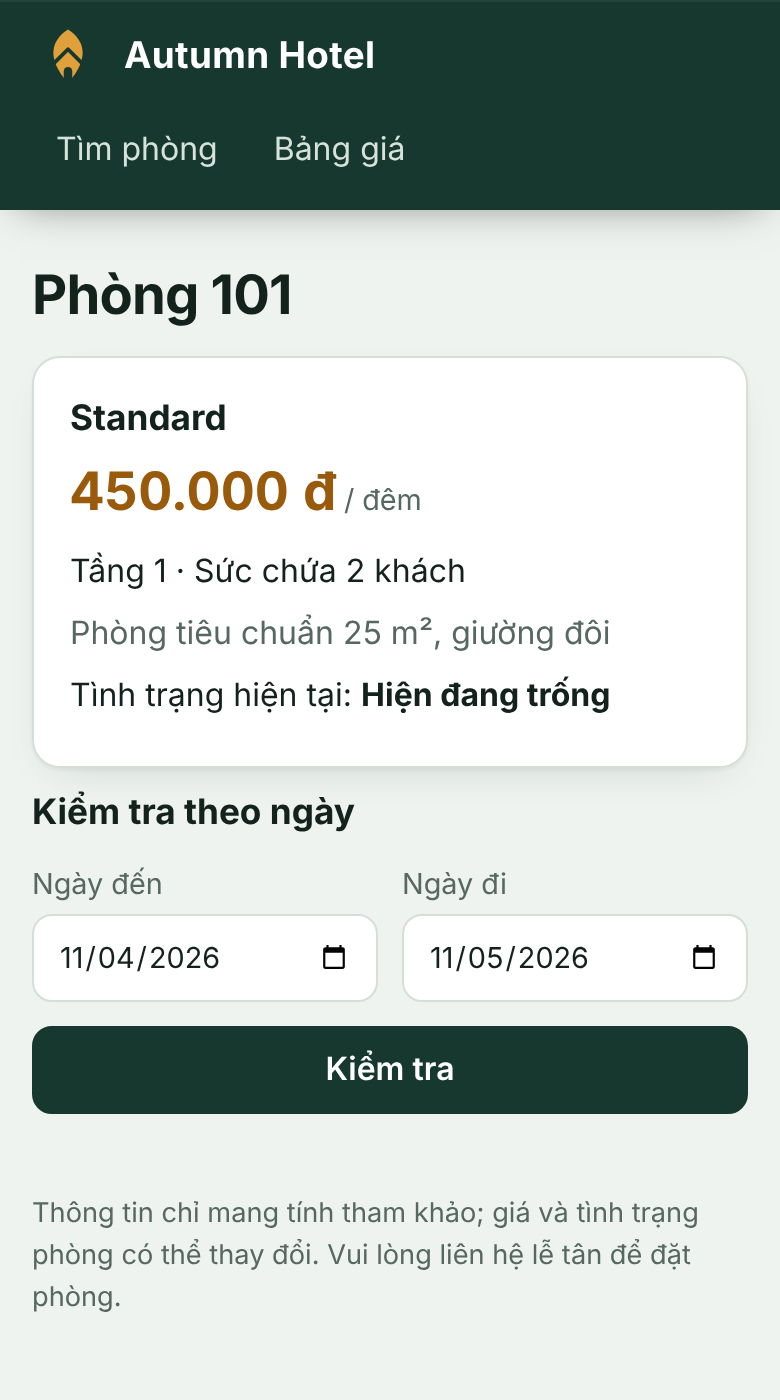
\includegraphics[width=0.45\textwidth]{WebPhong.png}}}{\fbox{\parbox{0.45\textwidth}{\centering\vspace{3cm}\textit{(Chèn ảnh chụp màn hình: WebPhong.png)}\vspace{3cm}}}}}
\caption{Trang chi tiết phòng trên điện thoại}
\label{fig:web-phong}
\end{figure}
\begin{figure}[H]
\centering
{\setlength{\fboxsep}{0pt}%
\IfFileExists{WebGia.png}{\fbox{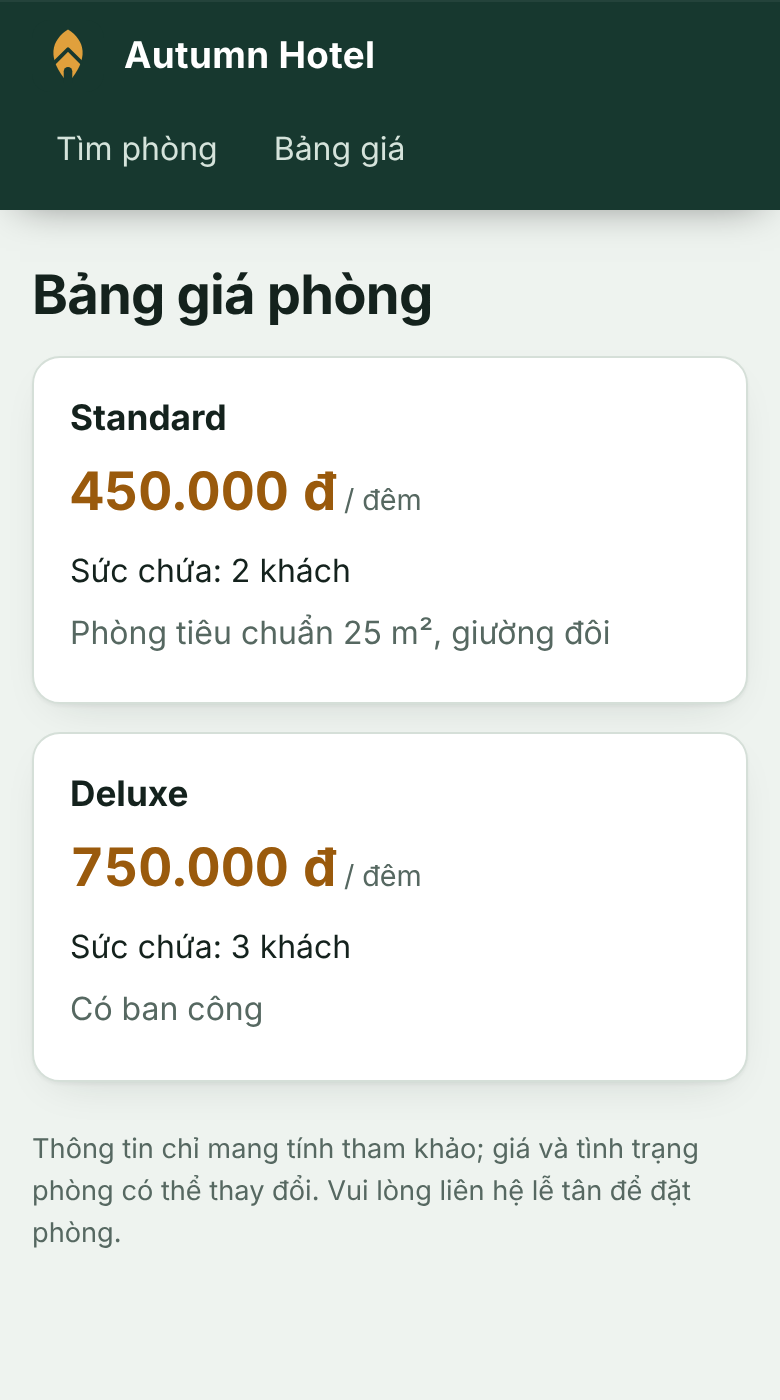
\includegraphics[width=0.45\textwidth]{WebGia.png}}}{\fbox{\parbox{0.45\textwidth}{\centering\vspace{3cm}\textit{(Chèn ảnh chụp màn hình: WebGia.png)}\vspace{3cm}}}}}
\caption{Trang bảng giá trên điện thoại}
\label{fig:web-gia}
\end{figure}

Việc trình bày các hình minh họa giao diện trong chương này dưới dạng khung mô tả bố cục (thay vì ảnh chụp màn hình thật) nhằm giữ cho báo cáo mô tả đúng thiết kế đã thống nhất của nhóm; ảnh chụp màn hình thực tế từ ứng dụng đang chạy có thể được bổ sung ở bản in cuối cùng khi chạy trên môi trường có SQL Server cấu hình đầy đủ.

% ===== end chuong/chuong7.tex =====

% ===== begin chuong/chuong8.tex =====
\chapter{Cài đặt, kiểm thử và đánh giá kết quả}

\section{Môi trường triển khai}

\begin{table}[H]
\centering
\caption{Môi trường phát triển và chạy ứng dụng}
\begin{tabularx}{\textwidth}{|l|X|}
\hline
\textbf{Thành phần} & \textbf{Phiên bản / Ghi chú} \\\hline
Ngôn ngữ & C\#, target \texttt{net10.0-windows} \\\hline
Giao diện & Windows Forms \\\hline
IDE & Visual Studio 2026 (18.0 trở lên) với .NET 10 SDK \\\hline
Cơ sở dữ liệu & Microsoft SQL Server (Express/Developer Edition) \\\hline
Cổng web (mở rộng) & ASP.NET Core, target \texttt{net10.0}, dự án \texttt{QuanLyKhachSan.Web}; cổng mặc định 5080 \\\hline
Cấu hình kết nối & \texttt{appsettings.json} (chỉ chứa cấu hình máy phát triển, không commit mật khẩu thật) \\\hline
Kiểm thử tự động & Project \texttt{QuanLyKhachSan.Tests}, chạy bằng \texttt{dotnet run} \\\hline
\end{tabularx}
\end{table}

\subsection{Các bước triển khai}

\begin{enumerate}
  \item Chạy lần lượt \texttt{QuanLyKhachSan/Scripts/01\_CreateDatabase.sql} (tạo database, bảng, ràng buộc, stored procedure) rồi \texttt{02\_InsertSampleData.sql} (dữ liệu mẫu và tài khoản demo) trên SQL Server; khuyến nghị dùng \texttt{sqlcmd -f 65001 -i <tên script>} để giữ đúng mã hóa tiếng Việt UTF-8.
  \item Kiểm tra \texttt{appsettings.json} trỏ đúng tới instance SQL Server đang chạy.
  \item Mở \texttt{QuanLyKhachSan.sln} bằng Visual Studio, build và chạy project \texttt{QuanLyKhachSan}.
  \item Đăng nhập bằng tài khoản mẫu đã seed sẵn trong script (một tài khoản Quản lý, một tài khoản Lễ tân).
  \item (Tùy chọn) Chạy \texttt{dotnet run --project QuanLyKhachSan.Web}; đặt \texttt{Web:BaseUrl} trong \texttt{QuanLyKhachSan/appsettings.json} thành địa chỉ IP nội bộ của máy chạy web, mở cổng 5080 trên tường lửa, rồi tạo mã QR từ menu \textit{Tra cứu}.
\end{enumerate}

\section{Kịch bản và kết quả kiểm thử}

\subsection{Kiểm thử logic tự động (độc lập CSDL)}

Project \texttt{QuanLyKhachSan.Tests} kiểm tra trực tiếp các quy tắc nghiệp vụ không phụ thuộc kết nối CSDL: số đêm lưu trú tối thiểu (QT40), phụ thu trả muộn theo ba mốc 1/3/6 giờ (QT43), tổng thanh toán không âm (QT45), giới hạn tiền cọc theo số đêm (QT15), gom doanh thu theo ngày/tháng/loại phòng kể cả các ngày không phát sinh giao dịch, tính tỷ lệ công suất trung bình, và xuất CSV (thoát dấu phẩy, dấu nháy kép, chặn chèn công thức). Bộ kiểm thử cũng bao phủ phần chức năng mở rộng: bộ mã hóa QR và lớp tạo đường dẫn tra cứu (QT65--QT68), quy tắc đổi phòng (QT47--QT49), bộ lọc tìm phòng và hình minh họa của cổng web (QT71), và phần logic thuần của cổng web (đọc/kiểm tra khoảng ngày, nhãn tình trạng phòng, giới hạn 60 đêm, mã hóa HTML chống chèn mã, định dạng giá, liên kết phòng). Bộ kiểm thử còn có nhóm kiểm thử Presenter (76 ca) chạy với View và Service giả, không mở giao diện và không cần CSDL: đăng nhập (khóa 30 giây sau 5 lần sai, đồng hồ giả), đặt phòng, nhận phòng, ghi dịch vụ, trả phòng (giảm giá trên 10\% cần Quản lý duyệt, hủy duyệt thì dừng), đổi phòng, duyệt giảm giá và báo cáo. Tổng cộng \textbf{208/208 ca kiểm thử đạt}.

\subsection{Kiểm thử SQL và build}

Bảng~\ref{tab:db-test} tóm tắt các kịch bản kiểm thử ở tầng CSDL; các thao tác tạo dữ liệu thử nghiệm được bọc trong transaction và rollback sau khi assert, không giữ lại bản ghi thử trong CSDL thật.

\begin{table}[H]
\centering
\caption{Kịch bản kiểm thử SQL và build}
\label{tab:db-test}
\begin{tabularx}{\textwidth}{|c|X|X|}
\hline
\textbf{ID} & \textbf{Kịch bản} & \textbf{Kết quả ghi nhận} \\\hline
DB-01 & Chạy script trên database thử nghiệm chưa tồn tại & Tạo database, 10 bảng, 6 stored procedure và dữ liệu mẫu; đạt \\\hline
DB-02 & Chạy lại script trên cùng database & Không tạo trùng object hay dữ liệu seed; đạt \\\hline
DB-03 & Kiểm tra lịch của phiếu thuê đang ở & \texttt{sp\_KiemTraTrungLich} phát hiện đúng trường hợp giao nhau, không báo khi liền kề; đạt \\\hline
DB-04 & Thêm dịch vụ và trả phòng trong transaction thử nghiệm & Hóa đơn 400.000đ tiền phòng + 30.000đ dịch vụ = 430.000đ; đạt \\\hline
DB-05 & Đặt phòng có khoảng ngày giao với đặt phòng đang hiệu lực & Bị từ chối do trùng lịch; đạt \\\hline
DB-06 & Chạy lại script và kiểm tra chỉ mục & Script chạy ổn định hai lần, đủ 6 index kiểm tra, gồm index lọc; đạt \\\hline
BUILD-01 & \texttt{dotnet build} toàn bộ solution & build thành công trên Windows, .NET 10; đạt \\\hline
\end{tabularx}
\end{table}

\subsection{Kiểm thử SQL và build tự động}

Tệp \texttt{.github/workflows/kiem-thu.yml} cấu hình GitHub Actions chạy mỗi lần đẩy mã lên nhánh chính với hai công việc. Công việc thứ nhất dùng SQL Server 2022 trong container, chạy hai script \texttt{01\_CreateDatabase.sql} và \texttt{02\_InsertSampleData.sql} hai lần (tạo mới và chạy lại) rồi chạy \texttt{Scripts/KiemThu.sql}. Script này gồm 34 ca: đủ 10 bảng, 6 thủ tục và các index; ràng buộc CHECK; kiểm tra trùng lịch; nhận phòng, ghi dịch vụ, trả phòng và hóa đơn; đổi phòng (các mã lỗi 50012 đến 50015, trạng thái phòng, lịch sử, dịch vụ giữ nguyên, tính tiền theo đơn giá ban đầu); thống kê doanh thu , công suất theo từng chặng phòng khi có đổi phòng và duyệt giảm giá trên 10\%. Công việc thứ hai trên Windows với .NET 10 biên dịch toàn bộ solution và chạy bộ kiểm thử logic 208 ca. Kết quả: cả hai công việc đạt, 34/34 ca SQL và 208/208 ca logic.

Quá trình này phát hiện và khắc phục một lỗi thiết kế: ràng buộc \texttt{UNIQUE} trên cột \texttt{MaDatPhong} (cho phép NULL) chỉ cho phép một phiếu thuê không có đặt phòng, làm khách vãng lai thứ hai không nhận được phòng. Ràng buộc được thay bằng unique index có điều kiện \texttt{WHERE MaDatPhong IS NOT NULL}; script tự chuyển đổi cơ sở dữ liệu cũ.

Các kết quả DB-01 đến BUILD-01 lấy từ lần chạy GitHub Actions gần nhất (SQL Server 2022, Windows với .NET 10). Kết quả giao diện vẫn do nhóm kiểm tra thủ công và không suy ra từ việc script hoặc build thành công.

\subsection{Kiểm thử giao diện thủ công}

Bảng~\ref{tab:ui-test} liệt kê các kịch bản kiểm thử giao diện cần thực hiện thủ công trên máy có SQL Server cấu hình đúng.

\begin{longtable}{|c|p{5.5cm}|p{5.3cm}|}
\caption{Kịch bản kiểm thử giao diện}\label{tab:ui-test}\\
\hline
\textbf{ID} & \textbf{Kịch bản} & \textbf{Kết quả mong đợi}\\\hline
\endfirsthead
\hline \textbf{ID} & \textbf{Kịch bản} & \textbf{Kết quả mong đợi}\\\hline
\endhead
UI-01 & Đăng nhập sai / tài khoản bị khóa & Từ chối đăng nhập, không mở màn hình chính \\\hline
UI-02 & Đăng nhập admin và lễ tân & Menu quản trị/báo cáo chỉ hiện với Quản lý \\\hline
UI-03 & Đổi mật khẩu sai hoặc xác nhận không khớp & Không cập nhật mật khẩu \\\hline
UI-04 & Tạo đặt phòng ngày đến $\ge$ ngày đi hoặc trùng lịch & Báo lỗi, không lưu \\\hline
UI-05 & Nhận phòng, ghi dịch vụ, trả phòng & Tạo phiếu, snapshot đơn giá, một hóa đơn duy nhất, phòng sang Dọn dẹp \\\hline
UI-06 & Trả phòng lần nữa cùng phiếu & Từ chối, không tạo hóa đơn thứ hai \\\hline
UI-07 & Tìm và xem trước/in hóa đơn & Nội dung in khớp hóa đơn được chọn \\\hline
UI-08 & Tạo khách với giấy tờ/điện thoại sai định dạng & Service báo lỗi trước khi gọi Repository \\\hline
UI-09 & Trả phòng rồi xác nhận dọn xong trên sơ đồ & Phòng chuyển Dọn dẹp $\to$ Trống hoặc Đã đặt nếu có lịch kế tiếp \\\hline
UI-10 & Đặt phòng tương lai cho phòng đang có khách/đang dọn & Chỉ chọn được phòng không giao lịch \\\hline
UI-11 & Đánh dấu Không đến / hủy rồi đặt lại cùng phòng, ngày & Phòng được giải phóng, đặt lại được \\\hline
UI-12 & Lễ tân mở danh mục; Quản lý mở báo cáo công suất & Lễ tân chỉ xem; Quản lý thấy biểu đồ, in, xuất CSV \\\hline
UI-13 & Mở \textit{Mã QR phòng và giá}, chọn phòng, lưu PNG rồi quét bằng điện thoại & Mở đúng trang \texttt{/phong/\{số\}}; mã còn quét được khi in \\\hline
UI-14 & Bật/tắt giao diện tối bằng Ctrl+D khi đang mở nhiều cửa sổ, đóng và mở lại ứng dụng & Mọi cửa sổ đổi màu ngay, chữ đọc được; lựa chọn được ghi nhớ; báo cáo in vẫn nền sáng \\\hline
UI-15 & Mở trang web với số phòng không tồn tại, ngày sai định dạng, ngày đến trước hôm nay, khoảng quá 60 đêm & Thông báo lỗi thân thiện, không lộ thông tin kỹ thuật \\\hline
UI-16 & Ngắt kết nối CSDL rồi tải trang web & Trang 503 chung; không lộ chuỗi kết nối; không thấy tên khách ở bất kỳ trang nào \\\hline
UI-17 & Mở ứng dụng, xem biểu tượng cửa sổ, thanh tác vụ và màn hình chính & Logo hiển thị ở biểu tượng và cạnh lời chào; vẫn chạy bình thường nếu thiếu tệp logo \\\hline
UI-18 & Mở Đổi phòng (F8), chọn phòng đang ở, chọn phòng trống khác mức giá, nhập lý do và xác nhận & Có lời nhắc giá; phòng cũ sang Dọn dẹp, phòng mới sang Đang ở; lịch sử hiện một dòng; dịch vụ đã ghi còn nguyên; trả phòng sau đó tính theo đơn giá cũ \\\hline
UI-19 & Đổi phòng khi phòng mới vừa bị đặt ở máy khác; đổi khi không còn phòng trống & Báo lỗi rõ, dữ liệu không đổi; thông báo không có phòng trống khi danh sách rỗng \\\hline
\end{longtable}

Các kịch bản UI là bước kiểm thử thủ công, thực hiện để kiểm tra bố cục (không bị chồng chéo, không bị cắt chữ) và đúng luồng nghiệp vụ; đây chưa phải kiểm thử tự động và kết quả UI không được suy diễn chỉ từ việc script SQL hay build thành công.

\section{Các lỗi đã phát hiện và khắc phục}

Trong quá trình hoàn thiện, nhóm phát hiện và sửa 10 lỗi, tổng hợp trong Bảng~\ref{tab:loi-da-sua}.

\begin{longtable}{|c|c|p{4cm}|p{5.7cm}|}
\caption{Lỗi đã phát hiện và khắc phục}\label{tab:loi-da-sua}\\
\hline
\textbf{\#} & \textbf{Mức} & \textbf{Lỗi} & \textbf{Cách sửa}\\\hline
\endfirsthead
\hline \textbf{\#} & \textbf{Mức} & \textbf{Lỗi} & \textbf{Cách sửa}\\\hline
\endhead
1 & Cao & Phụ thu trả muộn bị tính hai lần khi khách ở quá ngày đi dự kiến & \texttt{QuyTacTinhTien.TinhPhuThuTraMuon} đo đúng so với mốc 12:00 ngày trả thực tế \\\hline
2 & Cao & Cọc không bị giới hạn theo số đêm (QT15) & \texttt{DatPhongService.Them} kiểm tra cọc $\le$ giá 1 đêm $\times$ số đêm \\\hline
3 & Cao & Đặt phòng cho phòng không tồn tại, ngừng hoạt động hoặc đang bảo trì & \texttt{DatPhongRepository.KiemTraPhong} kiểm tra trong transaction Serializable \\\hline
4 & Cao & Phòng bị kẹt vĩnh viễn ở trạng thái "Dọn dẹp" & Thêm \texttt{PhongService.HoanTatDonDep} và thao tác xác nhận trên sơ đồ phòng \\\hline
5 & Trung bình & Repository tham chiếu ngược lên Service (vi phạm nguyên tắc phân lớp) & Chuyển kiểm tra cọc về đúng lớp Service \\\hline
6 & Trung bình & Không đánh dấu được "Khách không đến", không xóa được dòng dịch vụ & Thêm \texttt{DanhDauKhongDen}, \texttt{XoaDichVu} (chỉ khi phiếu còn "Đang ở") \\\hline
7 & Trung bình & Có thể khóa được tài khoản Quản lý cuối cùng & Kiểm tra trong transaction Serializable ở \texttt{NguoiDungRepository} \\\hline
8 & Giao diện & Số liệu thẻ thống kê và chữ "Làm mới" bị cắt; kích thước hàng/cột cố định & Viết lại bố cục bằng \texttt{TableLayoutPanel}/\texttt{FlowLayoutPanel} tự co, \texttt{MinimumSize}, cỡ thẻ phòng tính theo cỡ chữ \\\hline
9 & Giao diện & Tô màu nút theo nội dung chữ hiển thị (dễ sai khi đổi ngôn ngữ/nhãn) & Nút hành động chính đánh dấu bằng thuộc tính \texttt{Tag = "chinh"} thay vì so khớp chuỗi \\\hline
10 & Giao diện & Chưa có biểu đồ, in báo cáo, xuất CSV & Bổ sung \texttt{ChartPanel}, \texttt{InAn}, \texttt{CsvExporter} \\\hline
\end{longtable}

Việc ghi nhận đầy đủ cả các lỗi \emph{đã sửa} thay vì chỉ trình bày sản phẩm cuối cùng giúp báo cáo phản ánh đúng quá trình lặp đi lặp lại giữa thiết kế, cài đặt và kiểm thử -- đặc biệt các lỗi mức Cao (\#1--\#4) đều liên quan trực tiếp tới các quy tắc nghiệp vụ QT15, QT43 và ràng buộc trạng thái phòng, cho thấy tầm quan trọng của việc kiểm thử kỹ các quy tắc tính tiền và quản lý trạng thái.

\section{Checklist bảo mật}

Bảng~\ref{tab:bmbd} tổng hợp 9 hạng mục bảo mật cơ bản đã rà soát.

\begin{table}[H]
\centering
\caption{Checklist bảo mật cơ bản}
\label{tab:bmbd}
\begin{tabularx}{\textwidth}{|X|c|X|}
\hline
\textbf{Hạng mục} & \textbf{Tình trạng} & \textbf{Ghi chú} \\\hline
Truy vấn có tham số & Đạt & Dùng \texttt{SqlParameter}; \texttt{RowFilter} đã thoát ký tự đặc biệt \\\hline
Băm mật khẩu & Đạt & PBKDF2 kèm salt riêng, số vòng lặp lưu trong CSDL \\\hline
Mật khẩu mạnh & Đạt & $\ge 8$ ký tự, chữ hoa/thường và số \\\hline
Giới hạn đăng nhập sai & Đạt (phía ứng dụng) & Khóa 30 giây sau 5 lần sai \\\hline
Phân quyền & Đạt & Menu ẩn/khóa theo vai trò, Service kiểm tra lại \\\hline
Luôn còn Quản lý hoạt động & Đạt & Transaction Serializable \\\hline
Chuỗi kết nối & Cần lưu ý & Không commit mật khẩu thật; dùng tài khoản SQL quyền tối thiểu khi triển khai thật \\\hline
Xuất CSV & Đạt & Chặn ký tự mở đầu công thức (\texttt{= + - @}) \\\hline
Thông báo lỗi & Đạt & Chỉ hiển thị lỗi nghiệp vụ, không lộ chuỗi kết nối \\\hline
\end{tabularx}
\end{table}

\section{Đánh giá kết quả đạt được}

Đối chiếu với danh sách 23 chức năng đã đặc tả ở Chương~1 (19 bắt buộc, 4 nâng cao) và các kịch bản kiểm thử ở trên, nhóm đánh giá: toàn bộ 19 chức năng bắt buộc đã được cài đặt và kiểm thử thủ công theo kịch bản UI-01 đến UI-12; toàn bộ 4 chức năng nâng cao (đổi phòng trong lúc lưu trú, thống kê công suất, sơ đồ phòng theo tầng, xuất CSV) đã hoàn thành; riêng đổi phòng kiểm tra theo kịch bản UI-18, UI-19. Ba chức năng mở rộng (giao diện sáng/tối, mã QR, cổng web tra cứu) được kiểm tra theo các kịch bản UI-13 đến UI-17 và WEB-01 đến WEB-08. Bộ kiểm thử logic tự động đạt 208/208 ca.

% ===== end chuong/chuong8.tex =====


% ================= KẾT LUẬN =================
\chapter*{KẾT LUẬN VÀ HƯỚNG PHÁT TRIỂN}
\TieuDeDau{KẾT LUẬN VÀ HƯỚNG PHÁT TRIỂN}
\addcontentsline{toc}{chapter}{KẾT LUẬN VÀ HƯỚNG PHÁT TRIỂN}
% ===== begin chuong/ket_luan.tex =====
\section*{1. Kết quả đạt được}
\addcontentsline{toc}{section}{1. Kết quả đạt được}

Qua quá trình thực hiện, nhóm đã xây dựng hoàn chỉnh một ứng dụng quản lý khách sạn theo mô hình MVP~\cite{potel} (View -- Presenter -- Service -- Repository, dùng chung các lớp Model), bao phủ 19/19 chức năng bắt buộc và 4/4 chức năng nâng cao đã đặc tả ở Chương~1. Hệ thống hiện thực đầy đủ chu trình nghiệp vụ từ đặt phòng, nhận phòng, ghi nhận dịch vụ, trả phòng, lập hóa đơn đến báo cáo doanh thu và công suất phòng, với các ràng buộc toàn vẹn dữ liệu quan trọng (kiểm tra trùng lịch bằng giao dịch Serializable, snapshot giá, UNIQUE trên hóa đơn theo phiếu thuê) được đảm bảo ở tầng cơ sở dữ liệu chứ không chỉ ở tầng ứng dụng. Về bảo mật, hệ thống áp dụng băm mật khẩu PBKDF2, truy vấn tham số hóa, giới hạn đăng nhập sai và phân quyền hai lớp (giao diện và Service). Bộ kiểm thử logic tự động đạt 208/208 ca (quy tắc tính tiền, báo cáo, CSV, mã QR và logic cổng web và các Presenter chạy với View giả). Mười lỗi phát hiện trong quá trình hoàn thiện (4 lỗi mức cao liên quan trực tiếp tới các quy tắc nghiệp vụ QT15, QT43 và ràng buộc trạng thái phòng) đã được khắc phục và ghi nhận đầy đủ trong Chương~8.

Về mặt tổ chức,  đã áp dụng cách phân chia công việc theo trục kỹ thuật dọc (mỗi người phụ trách trọn một nhóm chức năng từ CSDL đến giao diện) thay vì phân chia ngang theo lớp kiến trúc, giúp giảm phụ thuộc chờ đợi lẫn nhau và phù hợp với quy mô nhóm nhỏ.

Ngoài phạm vi đặc tả ban đầu, nhóm đã bổ sung ba tính năng mở rộng. Thứ nhất, chế độ giao diện sáng/tối chuyển đổi bằng phím tắt Ctrl+D, áp dụng ngay cho các cửa sổ đang mở và được ghi nhớ giữa các lần chạy; bản in báo cáo luôn dùng nền sáng. Thứ hai, chức năng tạo mã QR tra cứu phòng và giá (menu Tra cứu), dùng bộ mã hóa QR do nhóm tự cài đặt (chế độ byte UTF-8, mức sửa lỗi M, phiên bản 1--10, mã Reed--Solomon trên GF(256)) nên không phụ thuộc thư viện ngoài; bộ kiểm thử tự động bổ sung thêm các ca cho bộ mã hóa QR và đường dẫn tra cứu, nâng tổng số lên 208 ca đạt (kể cả phần logic của cổng web, bộ lọc, quy tắc đổi phòng và các Presenter MVP), và các mã QR sinh ra đã được giải mã đúng bằng thư viện OpenCV. Thứ ba, cổng web chỉ đọc \texttt{QuanLyKhachSan.Web} (ASP.NET Core) dùng chung các lớp Model/Repository/Service với ứng dụng WinForms, cho phép khách quét mã QR để xem giá, tình trạng phòng và phòng trống theo ngày; trang công khai không hiển thị thông tin khách, mọi dữ liệu xuất ra đều được mã hóa HTML và lỗi cơ sở dữ liệu chỉ được ghi log nội bộ.

\section*{2. Hạn chế}
\addcontentsline{toc}{section}{2. Hạn chế}

\begin{itemize}
  \item Khi đổi phòng giữa hai loại phòng khác giá, đơn giá phiếu thuê được giữ nguyên và chênh lệch xử lý thủ công khi trả phòng.
  \item Các kịch bản kiểm thử giao diện (UI-01 đến UI-19) là kiểm thử thủ công, chưa được tự động hóa bằng công cụ kiểm thử giao diện chuyên dụng.
  \item Ứng dụng hiện chỉ hỗ trợ một máy trạm kết nối trực tiếp tới một CSDL tập trung, chưa tính tới kịch bản nhiều chi nhánh hoặc truy cập đồng thời ở quy mô lớn.
  \item Trạng thái khóa đăng nhập sau 5 lần sai được giữ trong bộ nhớ của màn hình đăng nhập, nên khởi động lại ứng dụng sẽ xóa trạng thái này; chưa lưu số lần sai và thời điểm khóa theo tài khoản trong CSDL.
  \item Chưa có chức năng xuất báo cáo ra định dạng Excel (.xlsx), hiện chỉ hỗ trợ xuất CSV.
  \item Cổng web hiện chỉ cho tra cứu (chưa cho khách tự đặt phòng) và chưa có xác thực hay HTTPS; muốn điện thoại quét được mã QR cần cấu hình địa chỉ mạng nội bộ (\texttt{Web:BaseUrl}) và mở cổng trên tường lửa.
\end{itemize}

\section*{3. Hướng phát triển}
\addcontentsline{toc}{section}{3. Hướng phát triển}

\begin{enumerate}
  \item Tách tiền phòng theo từng chặng giá khi đổi phòng giữa hai loại phòng khác giá.
  \item Mở rộng bộ kiểm thử tự động, bổ sung kiểm thử tích hợp có kết nối CSDL thử nghiệm.
  \item Bổ sung xuất báo cáo ra Excel, hỗ trợ định dạng và công thức tính sẵn cho người dùng tùy biến thêm.
  \item Nghiên cứu khả năng mở rộng thành mô hình nhiều chi nhánh, đồng bộ dữ liệu qua một CSDL trung tâm hoặc kiến trúc client-server mở rộng.
  \item Mở rộng cổng web chỉ đọc hiện có thành chức năng khách tự đặt phòng (kèm xác thực, HTTPS và giới hạn tần suất truy cập), tái sử dụng lớp Service để không phải viết lại logic nghiệp vụ; các điểm cuối JSON sẵn có (\texttt{/api/gia}, \texttt{/api/phong-trong}) cũng là nền tảng cho ứng dụng di động.
  \item Hoàn thiện giao diện tối (hiện là bộ màu tự cài đặt, chưa dùng thư viện giao diện chuyên dụng) và kiểm tra trên nhiều phiên bản Windows, đặc biệt các điều khiển hệ thống như ô chọn ngày.
\end{enumerate}

% ===== end chuong/ket_luan.tex =====


% ================= TÀI LIỆU THAM KHẢO =================
% thebibliography tự tạo tiêu đề chương; đặt tên để không phát sinh trang trắng
\renewcommand{\bibname}{TÀI LIỆU THAM KHẢO}
\clearpage\phantomsection
\addcontentsline{toc}{chapter}{TÀI LIỆU THAM KHẢO}
% ===== begin chuong/tai_lieu_tham_khao.tex =====
% Danh mục theo định dạng IEEE, đánh số theo thứ tự xuất hiện trong báo cáo.
\begin{thebibliography}{99}
  \bibitem{potel} M. Potel, ``MVP: Model-View-Presenter --- The Taligent programming model for C++ and Java,'' Taligent, Inc., 1996.
  \bibitem{fowler} M. Fowler, ``Passive View,'' martinfowler.com, Jul. 18, 2006. [Online]. Available: \url{https://www.martinfowler.com/eaaDev/PassiveScreen.html}
  \bibitem{owasp-sqli} OWASP Foundation, ``SQL injection prevention cheat sheet,'' OWASP Cheat Sheet Series. [Online]. Available: \url{https://cheatsheetseries.owasp.org/cheatsheets/SQL_Injection_Prevention_Cheat_Sheet.html}
  \bibitem{rfc8018} K. Moriarty, Ed., B. Kaliski, and A. Rusch, ``PKCS \#5: Password-based cryptography specification version 2.1,'' Internet Engineering Task Force, RFC 8018, Jan. 2017, doi: 10.17487/RFC8018.
  \bibitem{uit-ptt} Trường Đại học Công nghệ Thông tin, ĐHQG-HCM, ``Tài liệu môn học Phân tích thiết kế hệ thống thông tin.'' [Online]. Available: \url{https://ctgt.uit.edu.vn/sach/phan-tich-thiet-ke-he-thong-thong-tin}
  \bibitem{thoai} L. T. Thoại, ``Tài liệu môn học Lập trình Windows.'' [Online]. Available: \url{https://thoailt.com}
  \bibitem{noibo} Nhóm thực hiện, ``Bộ tài liệu đặc tả nội bộ của dự án (thư mục \texttt{docs/}),'' tài liệu nội bộ, 2026.
  \bibitem{ms-winforms} Microsoft, ``Windows Forms documentation,'' Microsoft Learn. [Online]. Available: \url{https://learn.microsoft.com/dotnet/desktop/winforms/}
  \bibitem{iso18004} \emph{Information technology --- Automatic identification and data capture techniques --- QR Code bar code symbology specification}, ISO/IEC 18004:2015, 3rd ed., International Organization for Standardization, Geneva, Switzerland, 2015.
  \bibitem{ms-sqlclient} Microsoft, ``Microsoft.Data.SqlClient documentation,'' Microsoft Learn. [Online]. Available: \url{https://learn.microsoft.com/sql/connect/ado-net/microsoft-data-sqlclient}
  \bibitem{ms-tsql} Microsoft, ``Transact-SQL (T-SQL) reference,'' Microsoft Learn. [Online]. Available: \url{https://learn.microsoft.com/sql/t-sql/}
  \bibitem{gantt} ``Gantt chart,'' ScienceDirect Topics. [Online]. Available: \url{https://www.sciencedirect.com/topics/computer-science/gantt-chart}
  \bibitem{ms-isolation} Microsoft, ``SET TRANSACTION ISOLATION LEVEL (Transact-SQL),'' Microsoft Learn. [Online]. Available: \url{https://learn.microsoft.com/sql/t-sql/statements/set-transaction-isolation-level-transact-sql}
  \bibitem{nist-63b} P. A. Grassi \emph{et al.}, ``Digital identity guidelines: Authentication and lifecycle management,'' National Institute of Standards and Technology, Gaithersburg, MD, USA, NIST Special Publication 800-63B, Jun. 2017, doi: 10.6028/NIST.SP.800-63b.
  \bibitem{owasp-csv} OWASP Foundation, ``CSV injection,'' OWASP Community. [Online]. Available: \url{https://owasp.org/www-community/attacks/CSV_Injection}
  \bibitem{reed-solomon} I. S. Reed and G. Solomon, ``Polynomial codes over certain finite fields,'' \emph{J. Soc. Ind. Appl. Math.}, vol. 8, no. 2, pp. 300--304, Jun. 1960.
\end{thebibliography}

% ===== end chuong/tai_lieu_tham_khao.tex =====


% ================= PHỤ LỤC =================
\appendix
% ===== begin chuong/phu_luc.tex =====
\chapter{Danh sách tài liệu đặc tả nội bộ}

Trong quá trình thực hiện, nhóm duy trì song song 10 tài liệu đặc tả nội bộ (thư mục \texttt{docs/}), dùng làm nguồn tham chiếu trực tiếp cho các chương của báo cáo này. Bảng~\ref{tab:docs-list} liệt kê đầy đủ.

\begin{table}[H]
\centering
\caption{Danh sách tài liệu đặc tả nội bộ}
\label{tab:docs-list}
\begin{tabularx}{\textwidth}{|l|X|l|}
\hline
\textbf{Tệp} & \textbf{Nội dung} & \textbf{Chương tham chiếu} \\\hline
01\_PhamVi\_ChucNang.md & Phạm vi, danh sách 23 chức năng, đối chiếu source & Chương 1 \\\hline
02\_QuyTrinh\_NghiepVu.md & Quy trình tổng quát, vòng đời trạng thái & Chương 5 \\\hline
03\_QuyTac\_NghiepVu.md & Quy tắc nghiệp vụ QT01--QT70 & Chương 5 \\\hline
04\_UseCase.md & 19 use case, ma trận chức năng--vai trò & Chương 3 \\\hline
06\_ERD\_Review.md & Sơ đồ ERD, quyết định thiết kế & Chương 4 \\\hline
07\_KichBanKiemThu.md & Kịch bản kiểm thử SQL/build/giao diện & Chương 8 \\\hline
08\_Loi\_Da\_Sua.md & Nhật ký 10 lỗi đã phát hiện và sửa & Chương 8 \\\hline
09\_HuongDan\_Demo.md & Hướng dẫn cài đặt và kịch bản demo & Chương 8 \\\hline
10\_Checklist\_BaoMat.md & Checklist bảo mật cơ bản & Chương 8 \\\hline
\end{tabularx}
\end{table}

\chapter{Trích đoạn mã nguồn tiêu biểu}

\section{Lớp quy tắc tính tiền (QuyTacTinhTien.cs)}

\begin{lstlisting}[language=csharp, caption={Tính tổng thanh toán theo công thức QT41--QT45 (rút gọn)}]
public static class QuyTacTinhTien
{
    public static decimal TinhTongThanhToan(
        decimal giaApDung, int soDem, decimal tongTienDichVu,
        decimal phuThuTraMuon, decimal tienCoc, decimal tyLeGiamGia)
    {
        decimal tienPhong = giaApDung * Math.Max(1, soDem);
        decimal truocGiam = tienPhong + tongTienDichVu + phuThuTraMuon;
        decimal sauGiam = truocGiam * (1 - tyLeGiamGia);
        return Math.Max(0m, sauGiam - tienCoc);
    }

    public static decimal TinhPhuThuTraMuon(
        DateTime ngayTraDuKien, DateTime thoiDiemTraThucTe, decimal giaMotDem)
    {
        DateTime mocChuan = ngayTraDuKien.Date.AddHours(12);
        if (thoiDiemTraThucTe <= mocChuan) return 0m;

        double soGioTre = (thoiDiemTraThucTe - mocChuan).TotalHours;
        if (soGioTre <= 1) return 0m;
        if (soGioTre <= 3) return giaMotDem * 0.25m;
        if (soGioTre <= 6) return giaMotDem * 0.5m;
        return giaMotDem;
    }
}
\end{lstlisting}

\section{Kiểm tra trùng lịch đặt phòng (sp\_KiemTraTrungLich)}

\begin{lstlisting}[language=SQL, caption={Thủ tục kiểm tra trùng lịch theo khoảng nửa mở (rút gọn)}]
CREATE OR ALTER PROCEDURE sp_KiemTraTrungLich
    @MaPhong INT, @NgayNhan DATE, @NgayTra DATE
AS
BEGIN
    SET TRANSACTION ISOLATION LEVEL SERIALIZABLE;
    IF EXISTS (
        SELECT 1 FROM DatPhong
        WHERE MaPhong = @MaPhong
          AND TrangThai IN (N'Da dat', N'Da nhan phong')
          AND NgayNhanDuKien < @NgayTra AND NgayTraDuKien > @NgayNhan
    )
        SELECT CAST(1 AS BIT) AS TrungLich;
    ELSE
        SELECT CAST(0 AS BIT) AS TrungLich;
END
\end{lstlisting}

\section{Ví dụ cấu trúc bảng (CREATE TABLE Phong)}

\begin{lstlisting}[language=SQL, caption={Cấu trúc bảng Phong (rút gọn)}]
CREATE TABLE Phong (
    MaPhong INT IDENTITY PRIMARY KEY,
    SoPhong NVARCHAR(10) NOT NULL UNIQUE,
    Tang INT NOT NULL,
    MaLoaiPhong INT NOT NULL
        FOREIGN KEY REFERENCES LoaiPhong(MaLoaiPhong),
    TrangThai NVARCHAR(20) NOT NULL
        CHECK (TrangThai IN (N'Trong', N'Da dat', N'Dang su dung',
                              N'Don dep', N'Bao tri', N'Ngung hoat dong'))
);
\end{lstlisting}

\chapter{Danh sách tài khoản mẫu}

Script khởi tạo CSDL tạo sẵn hai tài khoản mẫu để phục vụ demo và kiểm thử: một tài khoản vai trò Quản lý (\texttt{admin}) và một tài khoản vai trò Lễ tân (\texttt{letan}), mật khẩu tương ứng được thiết lập trong \texttt{02\_InsertSampleData.sql} và nên được đổi lại trước khi triển khai môi trường thật, theo đúng khuyến nghị bảo mật tại Mục~8.4.
Bảng~\ref{tab:taikhoan-mau} liệt kê hai tài khoản được script \texttt{02\_InsertSampleData.sql} tự động khởi tạo (chỉ chèn nếu tên đăng nhập chưa tồn tại), dùng để đăng nhập lần đầu khi demo hoặc kiểm thử hệ thống.

\begin{table}[H]
\centering
\caption{Danh sách tài khoản mẫu}
\label{tab:taikhoan-mau}
\begin{tabularx}{\textwidth}{|l|l|l|X|}
\hline
\textbf{Tên đăng nhập} & \textbf{Mật khẩu} & \textbf{Vai trò} & \textbf{Ghi chú} \\\hline
admin & Admin@123 & Quản lý & Họ tên mẫu: "Quản lý đa năng"; đầy đủ quyền quản trị \\\hline
letan & Admin@123 & Lễ tân & Họ tên mẫu: "Lễ tân 0 lương"; chỉ quyền nghiệp vụ hằng ngày \\\hline
\end{tabularx}
\end{table}

Mật khẩu của cả hai tài khoản được băm bằng PBKDF2-SHA256 với 100.000 vòng lặp (\texttt{SoVongLap}) và salt riêng cho từng tài khoản, lưu trong cột \texttt{MatKhauHash}/\texttt{MatKhauSalt} của bảng \texttt{NguoiDung}; giá trị \texttt{Admin@123} trong Bảng~\ref{tab:taikhoan-mau} là mật khẩu gốc dùng để đăng nhập, không phải giá trị lưu trong CSDL. Mật khẩu này thỏa quy tắc QT62 (tối thiểu 8 ký tự, có chữ hoa, chữ thường và số) nhưng chỉ nên dùng cho mục đích demo/kiểm thử; cần đổi mật khẩu (chức năng HT02) hoặc tạo tài khoản mới trước khi triển khai trên môi trường thật, theo đúng khuyến nghị bảo mật tại Mục~8.4.

% ===== end chuong/phu_luc.tex =====


\end{document}